%                                     MMMMMMMMM        
%                                                                             
%  MMO    MM   MMMMMM  MMMMMMM   MM    MMMMMMMM   MMD   MM  MMMMMMM MMMMMMM   
%  MMM   MMM   MM        MM     ?MMM              MMM$  MM  MM         MM     
%  MMMM 7MMM   MM        MM     MM8M    MMMMMMM   MMMMD MM  MM         MM     
%  MM MMMMMM   MMMMMM    MM    MM  MM             MM MMDMM  MMMMMM     MM     
%  MM  MM MM   MM        MM    MMMMMM             MM  MMMM  MM         MM     
%  MM     MM   MMMMMM    MM   MM    MM            MM   MMM  MMMMMMM    MM
%
%
%            - META-NET Language Whitepaper | Catalan content -
% 
% ----------------------------------------------------------------------------

\begin{document}

\maketitle

\null
\pagestyle{empty} 

\makefundingnotice

\pagenumbering{Roman} 
\setcounter{page}{5}
\pagestyle{scrheadings}

\cleardoublepage

% --------------------------------------------------------------------------
\bsection*{Pròleg --- Preface}

\begin{Parallel}[c]{78mm}{78mm}
\ParallelLText{\selectlanguage{catalan}
Aquest document forma part d'una sèrie que vol donar a coneixer les tecnologies del llenguatge i el seu potencial. S'adreça a educadors, periodistes, polítics i membres de comunitats lingüístiques, entre d'altres.

A Europa, la disponibilitat de tecnologies del llenguatge i el seu ús varia segons l’idioma. En conseqüència, les accions que es requereixen per reforçar la investigació i el desenvolupament d'aquestes tecnologies també són diferents per a cada idioma. Les accions necessàries depenen de molts factors, com ara la complexitat d'una llengua determinada o de la mida de la comunitat de parlants.

META-NET, una xarxa d'excel·lència finançada per la Comissió Europea, ha dut a terme una anàlisi de l’estat actual dels recursos i les tecnologies del llenguatge per a les 23 llengües oficials europees, així com per a d’altres idiomes importants a nivell nacional i regional a Europa. Els resultats d'aquesta anàlisi suggereixen que hi ha encara mancances significatives en la investigació necessària per a cada idioma. Una anàlisi més detallada i una avaluació experta de la situació actual han de contribuir a maximitzar l'impacte de noves investigacions i minimitzar-ne els riscos. 

META-NET es compon de 54 centres de recerca de 33 països que estan treballant amb tots els agents implicats (p.~\pageref{metanetmembers}): comercials, agències de govern,  organitzacions de recerca, empreses de programari, proveïdors de tecnologia i universitats europees. Junts, estan treballant en una visió comuna de la tecnologia i desenvolupant una agenda estratègica de la recerca que mostra com les aplicacions de les tecnologies del llenguatge podran resoldre els problemes actuals abans de l’any 2020.}

\ParallelRText{\selectlanguage{english}
This white paper is part of a series that promotes knowledge about language technology and its potential. It addresses journalists, politicians, language communities, educators and others. 
The availability and use of language technology in Europe varies between languages. Consequently, the actions that are required to further support research and development of language technologies also differ. The required actions depend on many factors, such as the complexity of a given language and the size of its community.

META-NET, a Network of Excellence funded by the European Commission, has conducted an  analysis of current language resources and technologies in this white paper series (p.~\pageref{whitepaperseries}). The analysis focused on the 23 official European languages as well as other important national and regional languages in Europe. The results of this analysis suggest that there are tremendous deficits in technology support and significant research gaps for each language. The given detailed expert analysis and assessment of the current situation will help maximise the impact of additional research.

As of November 2011, META-NET consists of 54 research centres from 33 European countries (p.~\pageref{metanetmembers}). META-NET is working with stakeholders from economy (software companies, technology providers and users), government agencies, research organisations, non-governmental organisations, language communities and European universities. Together with these communities, META-NET is creating a common technology vision and strategic research agenda for multilingual Europe 2020.} 
\ParallelPar
\end{Parallel}

\cleardoublepage

% --------------------------------------------------------------------------
\bsection*{Sumari --- Table of Contents}

\renewcommand\contentsname{}

\tableofcontents
\addtocontents{toc}{\protect\thispagestyle{empty}\protect}
\addtocontents{toc}{{\Large\textsf{\centerline{La LLENGUA CATALANA A L'ERA DIGITAL}}\par}}

\cleardoublepage


% --------------------------------------------------------------------------
\setcounter{page}{1}
\pagenumbering{arabic} 
\pagestyle{scrheadings}


% Start of origin language part
% --------------------------------------------------------------------------
\ssection[Resum]{Resum}

\selectlanguage{Catalan}

\begin{multicols}{2}

Al llarg dels últims 60 anys, Europa s'ha anat convertint en una estructura política i econòmica ben definida, encara que culturalment i lingüísticament sigui molt diversa. És a dir, que la comunicació entre els ciutadans europeus,
tant la més quotidiana com la que es produeix en l'àmbit dels negocis o la política, ja sigui per portuguesos o polonesos, o per italians o islandesos, cal que superi inevitablement les barreres de l'idioma. Les institucions de la UE gasten prop de mil milions d'euros l'any per mantenir la seva política de multilingüisme, és a dir, la traducció de textos i la interpretació de comunicacions orals. Però, cal que la diversitat lingüística resulti una càrrega tan costosa? Les modernes tecnologies del llenguatge i la recerca lingüística poden contribuir de forma significativa a enderrocar aquestes barreres lingüístiques. Combinant adequadament els dispositius intel·ligents i les seves aplicacions amb les tecnologies del llenguatge es podrà, en un futur proper, ajudar als ciutadans europeus a comunicar-se fàcilment els uns amb els altres i fer negocis tot i no parlar cap llengua en comú.

    \boxtext{Les tecnologies del llenguatge construeixen ponts pel futur d'Europa}

L'economia europea treu un major profit del mercat únic europeu que d'altres: El 2010, el comerç dins de la UE significava el 60,3\% de les exportacions alemanyes mentre que el comerç amb altres països europeus era un 10,8\% de les mateixes, però les barreres lingüístiques poden aturar el progrés dels negocis, especialment en el cas de les PIME (Petita I Mitjana Empresa) que no tenen els mitjans econòmics per abordar aquesta situació. L'única (impensable) alternativa a aquesta Europa multilingüe seria permetre que una sola llengua prengui la posició dominant i acabi reemplaçant totes les altres llengües.

Una forma clàssica de superar les barreres lingüístiques és l'aprenentatge de llengües estrangeres, però, sense cap suport tecnològic, esdevenir un expert en les 23 llengües oficials dels Estats membres de la Unió Europea i en, aproximadament, les 60 llengües europees addicionals, és una tasca pràcticament impossible per qualsevol ciutadà i és un fre pel desenvolupament econòmic, el debat polític o el progrés científic d’Europa.

La solució passa per desenvolupar tecnologies clau que facilitin la comunicació. Aquestes tecnologies ofereixen avantatges enormes  en l'àmbit europeu, no només dins del mercat comú, sinó també en les relacions comercials amb tercers països, especialment en les economies emergents. Per aconseguir aquest objectiu i preservar la diversitat cultural i lingüística d'Europa, primer és necessari realitzar una anàlisi sistemàtica de les particularitats lingüístiques i de l'estat actual de la tecnologia de suport de cadascun dels idiomes europeus. En un futur proper, les solucions de les tecnologies del llenguatge podran ser un pont entre les llengües d'Europa.

La traducció automàtica i les eines de processament de la parla actualment disponibles al mercat encara són lluny d'un objectiu tan ambiciós. Els principals protagonistes de l'àmbit són empreses de propietat privada amb ànim de lucre radicades a Amèrica del Nord. Ja en la dècada de 1970, la UE es va adonar de la profunda rellevància de les tecnologies del llenguatge com a guia cap a la unitat europea, i va començar a finançar els seus primers projectes de recerca, per exemple EUROTRA. Al mateix temps, es van establir projectes nacionals que generaren valuosos resultats, però sense arribar a constituir una acció ben coordinada a nivell europeu. Contrastant amb aquest esforç de finançament selectiu, altres societats multilingües, com l'Índia (22 llengües oficials) i Sud-àfrica (11 llengües oficials) han creat recentment programes nacionals d'investigació lingüística i desenvolupament tecnològic a llarg termini.

Avui, els models predominants en tecnologies del llenguatge depenen de mètodes estadístics que no fan ús de mètodes o coneixements lingüístics profunds. Per exemple, les frases es tradueixen automàticament mitjançant la comparació d'una nova frase contra milers de frases prèviament traduïdes per humans. La qualitat de la traducció depèn en gran mesura de la quantitat i qualitat dels corpora de la mostra disponible. Mentre que la traducció automàtica d'oracions simples en idiomes amb una quantitat suficient de material de text disponibles poden donar resultats útils, els mètodes estadístics estan condemnats al fracàs en el cas d'idiomes amb una mostra de materials de traducció molt petita, o en la traducció d'oracions amb estructures complexes.

\boxtext{Tecnologies del llenguatge, com una clau per al futur}

La Unió Europea ha decidit finançar projectes com ara EuroMatrix i EuroMatrixPlus (des de 2006) o iTranslate4 (des de 2010) que fan recerca bàsica i aplicada i generen recursos per a l'establiment de solucions d'alta qualitat en tecnologies del llenguatge en tots els idiomes europeus. L'anàlisi de les propietats estructurals més profundes de les llengües és l'únic camí si volem crear aplicacions que funcionin bé en tot el rang de les llengües d'Europa.

La investigació europea en aquest àmbit ja ha aconseguit diversos èxits. Per exemple, els serveis de traducció de la Unió Europea utilitzen ara  MOSES un programari de traducció automàtica de codi font obert que s'ha desenvolupat gràcies principalment a projectes de recerca europeus. El projecte Verbmobil, finançat pel Ministeri alemany d'Educació i Investigació (BMBF) entre 1993 i 2000, va situar Alemanya al capdavant del món de la investigació en traducció de la parla durant un temps. Molts dels laboratoris de recerca i desenvolupament ubicats a Alemanya aleshores (com IBM o Philips) han anat tancant o s'han traslladat a un altre lloc des de llavors. En lloc de construir sobre els resultats dels seus projectes de recerca, Europa ha tendit a realitzar activitats aïllades amb poc impacte en el mercat. El valor econòmic dels primers esforços fins i tot es pot veure en el nombre de derivats posteriors. Una companyia com Trados, que va ser fundada el 1984, va ser venuda a la SDL, amb seu al Regne Unit, el 2005.

\boxtext{Les tecnologies del llenguatge ajuden a unificar Europa}

Segons l'estat actual de les tecnologies del llenguatge, sembla que les anomenades "tecnologies híbrides", que combinen processament a partir de coneixements lingüístics profunds amb mètodes estadístics, seran capaces de connectar totes les llengües europees i de molt més. Com aquesta sèrie de llibres blancs sobre les llengües europees demostra, hi ha grans diferències  pel que fa a inversions en solucions tecnològiques i a l'estat de la recerca lingüística entre els Estats membres d'Europa. El català és una de les llengües de la UE que necessita encara més investigació per tal que les solucions de les tecnologies del llenguatge siguin veritablement eficaces i estiguin a punt per a l’ús diari. Al mateix temps, hi ha bones perspectives per tal d'assolir una posició destacada en aquesta àrea tecnològica tan important.

 A llarg termini, l’objectiu de META-NET és introduir tecnologies del llenguatge d'alta qualitat  per a tots els idiomes per tal d'aconseguir una unitat política i econòmica a través de la diversitat cultural. La tecnologia ajudarà a enderrocar les barreres existents i a construir ponts entre les llengües d'Europa. Això requereix que totes les parts interessades - política, recerca, empreses i societat - uneixin els seus esforços per al futur.

Aquesta sèrie de llibres blancs complementa altres accions estratègiques adoptades per META-NET (vegeu l'apèndix per a una descripció). Les versions actualitzades dels documents “\textit{META-NET vision paper}” \cite{Meta1} o “\textit{Strategic Research Agenda (SRA)}” es poden trobar al lloc web de META-NET: \url{http://www.meta-net.eu}.
\end{multicols}

\clearpage


% --------------------------------------------------------------------------
\ssection[Un risc per a les nostres llengües i un repte per a les tecnologies del llenguatge]{Un risc per a les nostres llengües\newline  i un repte per a les\newline tecnologies del llenguatge}

\begin{multicols}{2}

Som testimonis d’una revolució digital que té un impacte espectacular en la comunicació i la societat. Els desenvolupaments recents en la tecnologia de comunicació digital i de xarxes es poden comparar a la invenció de la impremta de Gutenberg.

\boxtext{La revolució digital és comparable a la invenció de la impremta de Gutenberg.}

Què ens pot dir aquesta analogia sobre el futur de la societat de la informació europea i les nostres llengües en particular?

Després de la invenció de la impremta de Gutenberg, es van dur a terme grans avenços en la comunicació i en l’intercanvi de coneixement mitjançant esforços com el de la traducció de Luter de la Bíblia a la llengua comuna.

En els segles posteriors, s’han desenvolupat tècniques culturals per tractar millor el processament del llenguatge i l’intercanvi de coneixement: 
\begin{itemize}
\item l’estandardització ortogràfica i gramatical de les principals llengües van permetre la ràpida difusió de noves idees científiques i intel·lectuals;
\item el desenvolupament de les llengües oficials va fer possible que els ciutadans es comuniquessin dins determinades fronteres (sovint polítiques);
\item l’ensenyament i la traducció de llengües va permetre l’intercanvi lingüístic;
\item la creació de pautes bibliogràfiques i periodístiques va assegurar la qualitat i la disponibilitat del material imprès;
\item la creació de diferents mitjans com els diaris, la ràdio, la televisió, els llibres i altres formats va satisfer les diferents necessitats de comunicació. 
\end{itemize}
En els últims vint anys, la tecnologia de la informació ha ajudat a automatitzar i facilitar molts dels processos:
\begin{itemize}
\item el programari d’edició de textes substitueix la mecanografia i la composició tipogràfica;
\item El \textit{PowerPoint} de Microsoft substitueix les transparències per retroprojector;
\item el correu electrònic envia i rep documents molt més de pressa que el fax;
\item L’Skype permet fer trucades telefòniques a través d’Internet i organitzar reunions virtuals;
\item els formats de codificació d’àudio i de vídeo faciliten l’intercanvi de contingut multimèdia;
\item els motors de cerca proporcionen accés a pàgines web basat en paraules clau;
\item els serveis en xarxa com el Google Translate produeixen traduccions ràpides i aproximades;
\item les plataformes dels mitjans de comunicació socials faciliten la coŀlaboració i permeten compartir informació.
\end{itemize}
Tot i que aquestes eines i aplicacions són útils, actualment no permeten implementar de manera suficient una societat de la informació europea sostenible i multilingüe, una societat moderna i inclusiva, on la informació i els productes puguin circular lliurement.

\subsection{Les fronteres lingüístiques dificulten la societat de la informació europea}
  
No podem saber exactament com serà la societat de la informació del futur. Quan es tracta de discutir una estratègia energètica europea o una política d’afers estrangers comunes, voldríem poder escoltar com parlen els ministres d’afers estrangers en la seva llengua materna. Voldríem poder tenir una plataforma on la gent, que parla moltes llengües diferents i amb dominis molts variats d’aquestes llengües, poguessin discutir un tema en particular mentre la tecnologia recopila automàticament les seves opinions i genera breus resums. També voldríem poder parlar amb el departament de suport o informació d’una companyia d’assegurances de salut que es troba en un país estranger.

\boxtext{L'espai d'economia i informació ens enfrenta amb diferents idiomes, parlants i contingut.}

És clar que les necessitats de comunicació tenen una qualitat diferent en comparació a fa uns anys. Una economia global i l’espai d’informació ens confronten amb més llengües, parlants i continguts, i ens demanen una interacció més ràpida amb nous tipus de mitjans de comunicació. La popularitat actual dels mitjans de comunicació socials (Viquipèdia, \textit{Facebook}, \textit{Twitter} i \textit{YouTube}) és només la punta de l’iceberg. 

Avui en dia, podem transmetre gigabytes de text arreu del món en pocs segons abans de reconèixer que el text és en una llengua que no entenem. D’acord amb un informe recent demanat per la Comissió Europea, el 57\% dels usuaris d’Internet a Europa compren productes i serveis en llengües que no són la seva llengua materna. (L’anglès és la llengua estrangera més comuna seguida del francès, l’alemany i l’espanyol.) El 55\% dels usuaris llegeix continguts en una llengua estrangera mentre que només un 35\% utilitza una altra llengua per escriure correus electrònics o publicar comentaris a la web \cite{CAT-Nota1}. Fa uns anys, l’anglès podria haver estat la lingua franca de la web —la gran majoria de continguts era en anglès— però ara la situació ha canviat radicalment. La quantitat de continguts en altres llengües (particularment en àrab i en llengües asiàtiques)  s’ha disparat.

Sorprenentment, una bretxa digital omnipresent causada per les fronteres lingüístiques no ha aconseguit ser un punt de gaire interès en el discurs públic; no obstant, hi ha una pregunta a l’aire que es planteja de manera insistent: “Quines llengües europees prosperaran i persistiran en la informació en xarxa i la societat del coneixement?”

\subsection{Les nostres llengües en risc}

La impremta va contribuir a un inestimable intercanvi d’informació a Europa, però també va portar l’extinció de moltes llengües europees. Poques vegades s’imprimia res en llengües regionals i minoritàries. Com a conseqüència, moltes llengües com el còrnic o el dàlmata es veien restringides a formes orals de transmissió, la qual cosa limitava la seva adopció continuada, l’extensió i l’ús. 

\boxtext{La varietat de llengues a Europa és un dels seus béns culturals més rics i importants.}

Les aproximadament 80 llengües que hi ha a Europa constitueixen un dels seus valors culturals més rics i importants. La multitud de llengües europees és també una part vital del seu èxit social \cite{CAT-Nota2}. Mentre les llengües populars com l’anglès i l’espanyol mantindran sens dubte la seva presència en el mercat i la societat digitals emergents, moltes llengües europees podrien quedar fora de les comunicacions digitals i esdevenir llengües irrellevants per a la societat d'Internet; un fet que, sens dubte, no seria convenient.  D’una banda, es perdria una oportunitat estratègica i com a conseqüència, la posició global d’Europa es veuria debilitada. De l’altra, s’entraria en conflicte amb l’objectiu de la igualtat de participació per a tots els ciutadans europeus, independent de la llengua. D’acord amb un informe de la UNESCO sobre el multilingüisme, les llengües són un mitjà essencial per al gaudi dels drets fonamentals, com l’expressió política, l’educació i la participació en la societat \cite{CAT-Nota3}.

\subsection{Les tecnologies del llenguatge són una tecnologia clau}

En el passat, els esforços d’inversió s’han centrat en l’ensenyament de llengües i la traducció. D’acord amb algunes estimacions, per exemple, el mercat europeu de traducció, interpretació, localització de programari i globalització de llocs web era de 8.400 milions d’euros el 2008 amb un creixement anual previst del 10\% \cite{CAT-Nota3}. No obstant, aquesta capacitat existent no és suficient per satisfer les necessitats actuals i futures. 

Les tecnologies del llenguatge són una tecnologia clau que pot protegir i fomentar les llengües europees. Les tecnologies del llenguatge ajuden la gent a coŀlaborar, fer negocis, compartir coneixement i participar en debats socials i polítics independentment de les barreres lingüístiques o dels coneixements d’informàtica. Les tecnologies del llenguatge s’utilitzen com a ajuda per a les tasques del dia a dia, com ara escriure correus electrònics, fer una cerca en xarxa o reservar un bitllet d’avió. Ens beneficiem de les tecnologies del llenguatge quan:   
\begin{itemize}
\item trobem informació a través d’un motor de cerca a Internet;
\item comprovem l’ortografia i la gramàtica en un processador de textos;
\item mirem les recomanacions de productes en una botiga en xarxa;
\item escoltem les instruccions verbals d'un sistema de navegació;
\item traduïm pàgines web mitjançant un servei en xarxa.
\end{itemize}

Les tecnologies del llenguatge que es detallen en aquest article són una part essencial de les aplicacions innovadores del futur. Les tecnologies del llenguatge són típicament una tecnologia clau amb una gran ventall d’aplicacions com ara un sistema de navegació o un motor de cerca. Aquests llibres blancs se centren en la disponibilitat de tecnologies bàsiques per a cada llengua europea.

\boxtext{Europa necessita unes tecnologies del llenguatge robustes i assequibles per tots els idiomes europeus.}

Per mantenir una posició capdavantera en la innovació global, Europa necessitarà que les tecnologies del llenguatge per a totes les llengües europees estiguin disponibles, que siguin assequibles i que estiguin perfectament integrades en entorns de programari més grans.  Una experiència d’usuari interactiva, multimèdia i multilingüe no és possible sense les tecnologies del llenguatge.

\subsection{Oportunitats per a les tecnologies del llenguatge}

Les tecnologies del llenguatge poden fer que la traducció automàtica, la producció de continguts, el processament de la informació i la gestió del coneixement siguin possibles per a totes les llengües d’Europa. També poden afavorir el desenvolupament d’interfícies intuïtives  per a l'ús d'electrodomèstics, maquinària, vehicles, ordinadors i robots. Tot i que ja existeixen molts prototips, les aplicacions comercials i industrials encara es troben en les primeres etapes de desenvolupament. Els èxits recents en recerca i desenvolupament han creat un ventall real d’oportunitats. Amb la traducció automàtica, per exemple, ja s’obté una qualitat molt raonable per a textos de dominis específics, i les aplicacions experimentals proporcionen informació multilingüe i gestió del coneixement, així com la producció de continguts en moltes llengües europees.

Les aplicacions lingüístiques, els sistemes de diàleg i les interfícies d’usuari basades en la veu s’han trobat fins ara en dominis altament especialitzats, i sovint ofereixen un funcionament molt limitat. Hi ha un mercat enorme d’oportunitats en l’educació i en les indústries d’entre\-te\-ni\-ment per a la integració de les tecnologies del llenguatge als jocs, a les ofertes d'entre\-te\-ni\-ment educatiu, als entorns de simulació o als programes de capacitació. Els serveis d’informació mòbils, els programaris d’aprenentatge de llengua assistits per ordinador, els entorns d’ensenyament a distància, les eines d’autoavaluació i els programaris de detecció de plagi són només uns quants exemples més dels llocs on les tecnologies del llenguatge poden jugar un paper important. La popularitat de les aplicacions dels mitjans de comunicació socials com el \textit{Twitter} i el \textit{Facebook} deixen entreveure que hi ha una necessitat addicional de tecnologies del llenguatge sofisticades que puguin controlar els missatges, resumir debats, suggerir tendències d’opinió, detectar respostes emocionals, identificar les infraccions de drets d’autor o un mal ús del servei. 

Les tecnologies del llenguatge representen una gran oportunitat per a la Unió Europea molt recomanable tant des del punt de vista econòmic com cultural.  El multilingüisme a Europa ha esdevingut la norma.  Les empreses europees, les organitzacions i les escoles també són multinacionals i diverses. Els ciutadans es volen comunicar tot traspassant les fronteres lingüístiques que encara hi ha en el Mercat Comú Europeu. Les tecnologies del llenguatge poden ajudar a superar les barreres que encara queden mentre donen suport a l’ús lliure i obert de la llengua. A més a més, unes tecnologies del llenguatge multilingües i innovadores per a Europa també ens pot ajudar a comunicar-nos amb els nostres socis mundials i les seves comunitats multilingües. Les tecnologies del llenguatge donen suport a una gran quantitat d’oportunitats econòmiques internacionals.

\boxtext{Les tecnologies del llenguatge ajuden a superar les ``traves'' de la diversitat lingüística.}

Un dels camps actius en recerca és la utilització de les tecnologies del llenguatge per a operacions de rescat en zones de desastres. En aquests entorns d’alt risc, la precisió en la traducció pot esdevenir una qüestió de vida o mort. El mateix raonament s’aplica a l’ús de les tecnologies del llenguatge en la indústria sanitària. Els robots inteŀligents amb capacitats lingüístiques per tractar amb diverses llengües tenen el potencial de salvar vides. 

\subsection{Els reptes de les tecnologies del llenguatge}

Tot i que les tecnologies del llenguatge han fet progressos considerables durant els últims anys, el ritme actual de progrés tecnològic i d’innovació de productes és massa lent.

\boxtext{El ritme actual de progrés tecnològic és massa lent.}

Les tecnologies del llenguatge amb un ús molt estès, com ara les eines d’ortografia i gramàtica dels processadors de text, acostumem a ser monolingües, o només estan disponibles per a un cert grup de llengües. La traducció automàtica i els serveis en xarxa són exceŀlents a l’hora de crear una bona aproximació dels continguts d’un document. Però aquests serveis en xarxa i les aplicacions professionals de traducció automàtica estan plens de dificultats quan es necessiten traduccions molt precises i completes. 

A causa de la complexitat del llenguatge humà, modelar les nostres llengües amb programaris i provar-les en el món real és un procés llarg i costós que requereix compromisos de finançament sostingut. Europa ha de mantenir el seu paper pioner enfront dels reptes tecnològics d'una comunitat multilingüe.

\boxtext{El progrés tecnològic necessita accelerar-se.}

\subsection{Adquisició de la llengua}

Per il·lustrar com els ordinadors tracten el llenguatge i per què l’adquisició de la llengua és una tasca complicada, farem un cop d’ull a la manera com els humans adquireixen la primera i la segona llengua, i després farem un esquema de com treballen els sistemes de tecnologies del llenguatge.

Els humans adquirim les habilitats lingüístiques de dues maneres diferents. En primer lloc, un nadó aprèn una llengua escoltant la interacció entre parlants d’aquesta llengua. L’exposició a exemples lingüístics concrets per part dels seus usuaris, com els pares, els germans o altres membres de la família, ajuda els infants d’uns dos anys a produir les seves primeres paraules o frases curtes. Això només és possible gràcies a una disposició genètica per a aprendre llengües que els humans tenen.

Aprendre una segona llengua normalment requereix molt més esforç quan el nen no es troba immers en una comunitat lingüística de parlants nadius. En edat escolar, les llengües estrangeres normalment s’adquireixen a través de l’aprenentatge de la seva estructura gramatical, vocabulari i ortografia de llibres i materials educatius que descriuen el coneixement lingüístic en termes de regles abstractes, taules i textos d’exemple. Aprendre una llengua estrangera requereix molt temps i esforç, i esdevé més difícil amb l’edat.

\boxtext{Els éssers humans adquirim les habilitats lingüístiques de dues maneres diferents: aprenent d'exemples i aprenent les regles subjacents de l'idioma.}

Els dos tipus principals de sistemes de tecnologies del llenguatge adquireixen les capacitats lingüístiques d’una manera molt similar a la dels humans. Els mètodes estadístics permeten obtenir coneixement lingüístic a partir de grans coŀleccions de textos d’exemple. Si bé és suficient l'ús de text en un sol idioma per l’entrenament, per exemple, d'un corrector ortogràfic, per l’entrenament d'un sistema de traducció automàtica han d'estar disponibles textos paraŀlels en dos (o més) llengües. L'algorisme d'aprenentatge aprèn els patrons de com es tradueixen les paraules, frases curtes i oracions completes.

Aquest enfocament estadístic pot requerir milions d'oracions i augmenta el rendiment de qualitat amb la quantitat de text analitzat. Aquest és un del motius pels quals els proveïdors dels motors de cerca estan disposats a recopilar tant material escrit com sigui possible. La correcció ortogràfica en els processadors de text, la informació en xarxa disponible, i els serveis de traducció com el Google Search i el Google Translate es basen en un enfocament (basat en dades) estadístic.   

El gran avantatge dels mètodes estadístics és que la màquina aprèn ràpidament en cicles continus d’entrenament, tot i que la qualitat pot variar de manera arbitrària.

El segon enfocament de la tecnologia del llenguatge i la traducció automàtica en particular son els sistemes basats en regles. Experts en lingüística, lingüística computacional i informàtica codifiquen anàlisis gramaticals (regles de traducció) i compilen llistes de vocabulari (lexicons). Alguns dels principals sistemes de traducció automàtica basada en regles han estat objecte de constant desenvolupament durant més de vint anys. L’avantatge dels sistemes basats en regles és que els experts poden controlar més detalladament el processament del llenguatge. Això fa que sigui possible corregir sistemàticament els errors del programari i retornar informació detallada a l’usuari, especialment quan aquests sistemes basats en regles s’utilitzen per a l’aprenentatge de llengües. Però, degut a l'elevat cost d'aquests desenvolupaments, les tecnologies del llenguatge basades en regles fins ara han estat privatives de les llengües majoritàries o d'aquelles que han tingut un recolçament institucional.

	Com que els sistemes estadístics i els basats en regles tendeixen a complementar-se, la recerca actual està treballant en sistemes híbrids que combinin els avantatges de totes dues metodologies. Aquests estudis són encara als laboratoris i han tingut poca implantació en aplicacions industrials.
	
	En aquest capítol hem vist que moltes aplicacions ampliament usades en la societat de la informació depenen de les tecnologies del llenguatge. Degut a la seva comunitat multilingüe, això és particularment cert en l'espai econòmic i de la informació a Europa. Tot i que les tecnologies del llenguatge han progressat considerablement en els darrers anys, encara hi ha un gran potencial per a millorar la qualitat dels sistemes que treballen amb les llengües. En el que resta, descriurem l'estat actual de les tecnologies del llenguatge per al català. 
\end{multicols}

\clearpage


% --------------------------------------------------------------------------
\ssection[El català a la societat de la informació europea]{El català a la societat de la informació europea}

\begin{multicols}{2}

\subsection{Aspectes generals}

El català forma part de la família de llengües romàniques. La llengua catalana té uns 8 milions de parlants nadius, i hi ha gairebé 12 milions de persones que la poden parlar. És llengua cooficial en tres regions d’Espanya: Catalunya, les Illes Balears i la Regió de València, i també es parla en alguns pobles fronterers d’Aragó i Múrcia. És l’única llengua oficial d’Andorra i també es parla en el departament francès dels Pirineus Orientals (conegut com a Catalunya Nord), i a la ciutat italiana de l’Alguer a Sardenya.

\boxtext{La llengua catalana té uns 8 milions de parlants nadius.}

L’estatus actual del català no és el mateix en tots els llocs on es parla. A Catalunya, la majoria de la gent és bilingüe. Uns estudis realitzats durant l’any 2010 per l’Institut d’Estudis Catalans confirma que el 95.3\% de la població entén el català, el 60.6\% el pot escriure, i el 77.5\% el pot parlar, però aquesta última xifra puja al 96.4\% quan l’estudi es restringeix a les persones nascudes a Catalunya. A més a més, altres estudis com el Programa per a l’Avaluació d’Estudiants Internacionals (\textit{Programme for International Student Assessment}, PISA) 2010 revela que gairebé el 80\% de la població a Catalunya pot llegir en català.

Com es dirà més endavant en aquest capítol, la llengua catalana es pot estudiar en diversos països arreu del món, especialment en universitats d’Europa i de Nord-amèrica.

\subsection{Particularitats del català}

La llengua catalana es distingeix clarament en dialectes, cinc dels quals (septentrional, central, nord-occidental, baleàric i valencià) tenen regles de normalització especials. Es diferencien principalment en la pronunciació d’algunes vocals, en alguns mots gramaticals (ex. articles, pronoms possessius i altres pronoms) i també en algunes paraules del lèxic.

El català utilitza vuit sons vocàlics diferents i trenta-un sons consonàntics. Utilitza l’alfabet de 26 lletres més 2 d’addicionals, la \textit{ç} (‘ce trencada’) i el dígraf \textit{ŀl} (‘ela geminada’).

\boxtext{El català utilitza vuit sons vocàlics diferents i trenta-un sons consonàntics.}

Pel que fa a l’ordre de les paraules de les oracions o expressions en català, el patró principal utilitzat és Subjecte, Verb, Objecte. No obstant, el català té una estructura molt lliure i no resulta estrany l’ús d’elements clítics que canvien l’estructura bàsica. Per exemple, l’oració: ‘La Maria ens portà els regals a nosaltres’ també es pot dir: ‘A nosaltres ens portà els regals la Maria’ o ‘Els regals la Maria ens els portà’.

El català és una llengua \textit{pro-drop}, és a dir, és possible utilitzar la conjugació del verb sense el pronom personal que fa la funció de subjecte. 

En català, a diferència del francès o l’anglès, per exemple, no és possible separar construccions verbals que porten un verb auxiliar. Per exemple, en anglès podem dir: ‘\textit{I} \underline{had} \textit{always} \underline{done} \textit{this}’; o en francès: ‘\underline{‘j‘avais} \textit{toujours} \underline{fait}  \textit{ça}’. En català diem: ‘jo sempre \underline{he fet} això’, o ‘jo \underline{he fet} sempre això’, però ‘jo \underline{he} sempre \underline{fet} això’ és incorrecte.

Com ja s’ha dit anteriorment, les arrels lèxiques del català provenen principalment del llatí. D’entre les llengües romàniques més parlades, l’italià i el francès són les més properes al català, tant des del punt de vista lèxic com fonètic. Així doncs, els catalanoparlants poden entendre fàcilment l’italià o el francès. 

L’ortografia en català és més transparent que en anglès, però menys que en espanyol o italià. Per exemple, vocals com la \textit{a}, la \textit{e} i la \textit{o}, es poden pronunciar de manera diferent en alguns dialectes, en funció de si es troben en una síŀlaba tònica o no. O la \textit{b} i la \textit{v}, que tenen la mateixa pronunciació en molts dialectes. Els signes d’accentuació i les dièresis s’utilitzen en català per ajudar a marcar l’accent i la pronunciació d’algunes paraules.

\subsection{Desenvolupament recent}

Després de la guerra civil espanyola (1936-1939) i durant la dictadura del general Franco (1936-1975) la llengua i la cultura catalanes van ser perseguides i fortament discriminades. Es va prohibir l’ús del català a l’escola, en qualsevol actuació administrativa i en qualsevol sistema de comunicació i difusió (llibres, diaris, radio, televisió i cinema).

La societat civil, no obstant, va mantenir una activitat cultural important, molts cops en clandestinitat, que va permetre un relaxament en la prohibició als anys 1970s. A partir de 1974 es comencen a publicar diaris en català i a partir de 1978 es permet l’ensenyament del català a l’escola.

 “La Nova Cançó” és un moviment cultural i artístic que impulsa, a finals dels 50, la reivindicació de l’ús normal del català. Es forma el grup “Els setze jutges” al 1959, i els primers discs cantats en català apareixen al 1962.

Òmnium Cultural \cite{CAT-omniumcultural} va néixer al 1961 amb l’objectiu de protegir i de promocionar la cultura catalana. L’entitat es va crear en un moment històric on la cultura catalana es trobava censurada i perseguida per la dictadura franquista i per tant era una necessitat nacional recuperar-la i mantenir-la. Des d’aquest punt de vista, l’entitat va esdevenir una eina social i fonamental de resistència nacional i de suplència de les institucions catalanes, inexistents durant la dictadura. Actualment Òmnium genera debat, intervé i es posiciona davant les qüestions d’actualitat que afecten la societat civil catalana. També defensa i promou la llengua i la cultura catalanes i la identitat nacional de Catalunya.

L’any 1976 Ràdio 4, emissora pública espanyola d’àmbit regional, inicia les seves emissions exclusivament en català.

L’any 1983 TV3 fa la seva primera emissió de proves. TV3 és un canal de televisió, gestionat per l’ens públic Corporació Catalana de Mitjans Audiovisuals \cite{CAT-CCMA}, que emet tota la seva programació en català.

La producció cinematogràfica en català es reactiva a partir de la segona dècada dels anys 70, i es consolida amb l’aparició de TV3, tant pel que fa a producció pròpia, com a la incorporació de subtitulat de peŀlícules i doblatge.

El 1985 la Generalitat de Catalunya i l’Institut d’Estudis Catalans funden el TERMCAT \cite{CAT-TERMCAT}, un centre de terminologia de la llengua catalana. La seva missió és garantir el desenvolupament i la integració de la terminologia catalana en els sectors especialitzats i en la societat en general.

\subsection{Promoció de la llengua catalana}

Tal i com es recull a l’article 6 de l’Estatut d’Autonomia de Catalunya \cite{CAT-estatut}, la llengua pròpia de Catalunya és el Català. El català és la llengua d’ús normal en l’administració pública, mitjans de comunicació públics de Catalunya i és la llengua normalment emprada en ensenyament. El català i el castellà son llengües oficials a Catalunya. Els ciutadans de Catalunya tenen el dret i el deure de conèixer les dues llengües.

L’Institut d’Estudis Catalans \cite{CAT-IEC}, fundat el 1907 per Enric Prat de la Riba, té per objecte l’alta recerca científica i principalment la de tots els elements de la cultura catalana. 

Amb el retorn a la normalitat a finals dels anys 70, l’Institut d’Estudis Catalans s’estructura en cinc seccions. La secció Filològica, acompleix la funció d'acadèmia de la llengua catalana que l'Institut té encomanada. Aquesta funció comporta l'estudi científic de la llengua, l'establiment de la normativa lingüística i el seguiment del procés d'aplicació d'aquesta normativa en l'àmbit que li és propi: les terres de llengua i cultura catalanes. Com a resultat de la seva funció, l’IEC publica El Diccionari de la llengua catalana, segona edició de 2007. Aquest diccionari normatiu i general és també un instrument per a conrear i fer prosperar la llengua catalana.

Enciclopèdia Catalana \cite{CAT-enciclopedia} és un projecte privat sense ànim de lucre, nascut l’any 1965, que s’ha consolidat com a referència en la publicació i consulta de en català d’obres de temàtica diversa, destacant per la seves enciclopèdies i diccionaris.

L’Institut Ramon Llull \cite{CAT-Nota12} es va crear l’any 2002, per part del Govern de la Generalitat de Catalunya i el Govern de les Illes Balears. Té com a finalitat la projecció exterior de la llengua catalana i de la cultura que s’hi expressa en totes les seves modalitats, matèries i mitjans d’expressió, així com la seva difusió i l’ensenyament fora del domini lingüístic tenint en compte totes les seves modalitats i variants. Disposa de dues seus, Barcelona i Palma , i d’oficines a Berlin, Londres, Nova York i París.

El Consorci per a la Normalització Lingüística \cite{CAT-cpnl} és un ens creat a partir de la voluntat comuna de la Generalitat i de nombrosos ajuntaments, consells comarcals i diputacions amb l’objectiu de facilitar el coneixement, l’ús i la divulgació de la llengua pròpia de Catalunya en tots els àmbits. Una de les seves funcions principals és la formació i suport lingüístic adreçat a persones de parla no catalana.

\subsection{La llengua a l’educació}

A Catalunya, des de finals dels seixanta fins ara, unes 80 escoles, creades com a cooperatives de pares o professors, foren les pioneres en la recuperació de l’ús del català a l’educació. Aquestes escoles es van inspirar en la tradició pedagògica que existia abans de la Guerra Civil espanyola (1936) i van seguir el mètode de Maria Montessori.

Amb la recuperació de la democràcia després de la mort del dictador el 1975, la Constitució Espanyola del 1978 va reconèixer la pluralitat lingüística de l’estat. L’Estatut de Catalunya del 1979 i l’Estatut de les Illes Balears del 1983 van reconèixer el català com a llengua pròpia i oficial, juntament amb l’espanyol. L’Estatut de la Comunitat Valenciana del 1982 va reconèixer-ne el seu estatus com a llengua oficial amb el nom legal de valencià.

En aquells temps, després d’anys d’ex\-clu\-sió en l’educació, el català es va trobar en una situació de clar desavantatge respecte a l’espanyol. Per fer front a aquesta situació, els governs autonòmics van adoptar diferents estratègies.

A Catalunya, l’estratègia adoptada el 1983 fou l’anomenada immersió lingüística, inspirada en un programa dut a terme al Quebec (Canadà) per tractar amb una situació de contacte lingüístic similar al de les regions catalanoparlants d’Espanya. El model es basava en la idea que els nens no s’haurien de separar en funció de la seva llengua materna, perquè això crearia dos models d’escola diferents: un per als nens catalanoparlants i l’altre per als nens castellanoparlants. En la immersió lingüística, els nens, independentment de la llengua que parlen a casa, són escolaritzats totalment en català i aprenent a llegir i escriure en aquesta llengua. Quan els nens comencen a dominar la llengua de l’escola, s’introdueix gradualment l’espanyol en el currículum. D’aquesta manera, quan finalitza l’ensenyament obligatori, els estudiants, tenen un domini equivalent tant en català com en castellà, i són bilingües i billetrats, com revelen diversos estudis d’investigació \cite{CAT-Nota5}.

\boxtext{Gràcies a la immersió lingüística, els estudiants tenen un domini equivalent tant en català com en castellà al finalitzar l'ensenyament obligatori.}

A les Illes Balears les autoritats autonòmiques van adoptar un programa d’immersió lingüística similar al de Catalunya, mentre que el model adoptat a la Comunitat Valenciana establia diferents tipus de centres i programes en funció de la llengua materna de l’estudiant.

A França, al Departament de Pirineus Orientals (Llenguadoc-Rosselló) la situació del català és molt pitjor que la de les regions catalanoparlants d’Espanya. Tot i que el català és la llengua pròpia d’una part de la població, la llengua d’instrucció a l’escola és el francès. El 1976 es va crear La Bressola \cite{CAT-Nota6} a Perpinyà, com una xarxa de vuit escoles que van adoptar el programa d’immersió lingüística en català, com a mitjà de recuperació de l’ús d’aquesta llengua en el dia a dia de la gent de la regió. A banda d’aquesta iniciativa, també hi ha algunes escoles bilingües a la regió, en les quals l’escolarització es fa en francès i en català.

L’últim informe PISA dut a terme el 2009 revelava que els estudiants a Catalunya, amb una puntuació mitjana de 498, es trobaven per sobre de la nota mitjana de l’OCDE (494) i de la nota mitjana d’Espanya (481) en relació a la comprensió lectora \cite{CAT-Nota7}. Això significa que el fet que els nens fossin escolaritzats seguint el programa d’immersió lingüística, en el qual el català és el mitjà principal d’instrucció, no afectava el seu rendiment en la comprensió lectora de l’espanyol.

No obstant, l’informe PISA també mostra que hi ha una notable diferència entre les puntuacions obtingudes pels estudiants nadius (catalano- o castellanoparlants) i aquelles puntuacions obtingudes pels estudiants amb un rerefons migratori. Aquests resultats han reforçat la consciència pública sobre la importància de l’aprenentatge de llengües, amb una especial atenció en la integració social. 

A l’inici del segle XXI hi ha un nou repte per a les escoles catalanes: l’escolarització de molts estudiants en rerefons de migració. A diferència dels anys seixanta, en què els nouvinguts eren majoritàriament castellanoparlants, actualment, els nens provenen de molts països d’arreu del món i parlen moltes llengües diferents. Per fer front a aquesta situació el govern ha creat les “aules d’acollida”. Inspirades en el programa d’immersió lingüística, aquestes “aules d’acollida” es conceben com un suport temporal per als nouvinguts, mentre es troben en el procés d’adquisició de coneixements mínims per comunicar-se amb els seus companys de classe.

\subsection{Aspectes internacionals}

El català és una de les anomenades llengües minoritàries i ha estat reconeguda com a tal pel Consell d’Europa en el Capítol Europeu per a Llengües Regionals o Minoritàries, l’objectiu del qual és “protegir i promoure les regions històriques o les llengües minoritàries d’Europa”. La importància d’aquestes llengües es testifica pel fet que hi ha més de quaranta milions de ciutadans de la UE que les parlen.

Com a llengua minoritària, el català va ser representat a l’Oficina Europea de Llengües Minoritàries, creada el 1982 per iniciativa del Parlament Europeu. L’objectiu d’aquesta organització no governamental paneuropea ha estat fomentar el respecte cap a les llengües menys protegides dins de la UE i promoure la diversitat lingüística. El català és també una de les llengües tractades a la Mercator Network \cite{CAT-Nota8}, una xarxa de tres centres de recerca i documentació, l’objectiu principal de la qual és esdevenir un centre de recursos especialitzat i un servei d’informació relatius a les llengües minoritzades europees. La Mercator té tres branques, cadascuna de les quals es centra en un programa temàtic: educació, legislació i mitjans de comunicació.  

Si considerem totes les llengües que es parlen a Espanya, només l’espanyol té l’estatus de llengua oficial a la UE. No obstant, el novembre del 2004 el govern espanyol va lliurar a la UE la traducció de la Constitució Europea a les llengües de l’estat que també són oficials en els seus respectius territoris: català (amb el nom de català, utilitzat a Catalunya i les Illes Balears, i el nom de valencià, utilitzat a la Comunitat Valenciana), gallec i basc.

El 2005 el Consell de Ministres va reconèixer la possibilitat d’utilitzar altres llengües oficials a part de l’espanyol a les institucions europees. Després de signar alguns acords administratius amb algunes institucions de la UE, reconeixent un ús limitat i restringit del català, actualment l’estatus del català és el de llengua semioficial, una llengua de comunicació entre els ciutadans. Aquest estatus significa que els ciutadans poden escriure en català a aquestes institucions (Comissió Europea, Parlament Europeu, Consell, Defensor del Poble Europeu i Comitè de Regions), i, a la vegada, tenen el dret de rebre resposta en la mateixa llengua. Algunes publicacions i documentació oficial també es tradueixen al català. D’altra banda, a la Representació de la Comissió Europea a Barcelona, el català s’utilitza com a llengua habitual de comunicació amb els ciutadans (campanyes d’informació, publicacions, comunicats de premsa i pàgina web). 

La projecció internacional del català és força limitada. En el món de l’empresa a nivell internacional, l’ús del català és inexistent. De fet, l’anglès ha esdevingut la llengua comuna de comunicació tan a nivell escrit com oral. Actualment, des del punt de vista del client, algunes grans multinacionals utilitzen el català per tractar amb els seus clients catalans, com a valor afegit per als seus productes i com a millora dels seus serveis al client. Algunes d’aquestes empreses són Microsoft, IKEA o Toshiba.

Pel que fa a l’aprenentatge del català com a llengua estrangera, la situació és lleugerament millor. La Comissió Europea està desenvolupant un política activa en matèria de multilingüisme, l’objectiu de la qual és la preservació i la promoció de la diversitat lingüística a Europa, fomentant l’aprenentatge de llengües (incloses les llengües regionals i les minoritàries) i utilitzant el multilingüisme com a estímul per a la competitivitat. En aquest context, el Lifelong Learning Programme 2007-13 conté una selecció de projectes que promouen l’aprenentatge de llengües. Entre ells, el centre de recursos lingüístics en xarxa multilingüe Lingu@net Europa Plus \cite{CAT-Nota9} dóna suport i recursos a 20 llengües europees, inclòs el català. A més a més, una decisió important presa pels representants dels Estats Membres de la UE ha estat incloure el català, així com el basc i el gallec, a la llista de llengües que s’ofereixen als cursos intensius de llengua Erasmus de l’any acadèmic 2010-2011 \cite{CAT-Nota10}. Aquests cursos de llengua finançats per la UE tenen com a objectiu preparar els futurs estudiants d’Erasmus per al seu període d’estudi a les universitats catalanes, on s’utilitza el català com a llengua acadèmica i de comunicació.

Tot i ser una llengua minoritària, l’interès a aprendre català en universitats estrangeres es testifica pel fet que, en aquest moment (anys acadèmic 2010-11), més de 160 universitats d’arreu del món ofereixen estudis de llengua catalana \cite{CAT-Nota11}. Alguns dels països en què aquesta oferta és més àmplia són Alemanya (26), Estats Units (23), Regne Unit (21), França (20) i Itàlia (17). El català es pot estudiar a 11 universitats espanyoles. L’Institut Ramon Llull (IRL) \cite{CAT-Nota12}, un consorci constituït pels Governs de Catalunya i de les Illes Balears, és la institució que té com a objectiu promoure la llengua i la cultura catalanes internacionalment. L’IRL és part de la Fundació Ramon Llull, creada pel Govern d’Andorra, l’IRL, el Consell General dels Pirineus Orientals, la ciutat de l’Alguer i la Xarxa de Ciutats Valencianes. Aquesta fundació involucra els governs i les institucions de l’àmbit lingüístic català, en un intent d’unificar esforços per a un objectiu comú.

\boxtext{Més de 160 universitats d’arreu del món ofereixen estudis de llengua catalana.}

L’interès del govern català i de les institucions en la projecció internacional de la llengua i la cultura també es veu reflectida en l’organització de diferents esdeveniments internacionals on el català ha estat el convidat principal o el convidat d’honor, com la Fira del Llibre de Frankfurt del 2007 \cite{CAT-Nota13}, el CatalanDays 2009 (Nova York) \cite{CAT-Nota14} o l’Expolangues 2010 (París) \cite{CAT-Nota15}. També, en el món literari el PEN Català \cite{CAT-Nota16}, fundat el 1922 (només un any després de la fundació del PEN International per C.A. Dawson Scott), ha estat una plataforma per a la projecció internacional de la literatura catalana i els escriptors de l’àmbit lingüístic català.

\subsection{El català a Internet}

 Al contrari del que es podria esperar d’una llengua minoritària (després de tot, el català ocupa la posició 75 a la classificació de l’Ethnologue \cite{CAT-Nota17} de les llengües segons el nombre de parlants), quan es tracta de la presència a Internet la situació és radicalment diferent. Segons Lluís Collado, la persona responsable de Google Books i Google News a Espanya i Portugal, Google situa la llengua catalana entre les 10 i 15 llengües més actives del món a la web. Google considera el català una llengua amb una activitat que va més enllà de les fronteres del seu domini lingüístic.  

\boxtext{Google situa la llengua catalana entre les 10 i 15 llengües més actives a la web.}

L’associació WICCAC \cite{CAT-Nota18}, que aglutina administradors de web independents de l’àmbit lingüístic català que han creat les seves pàgines web en aquesta llengua, publica un baròmetre mensual sobre l’ús del català a Internet. El baròmetre s’actualitza mitjançant enquestes als llocs web d’empreses i organitzacions ubicades a Catalunya o altres llocs del domini lingüístic. L’enquesta també inclou les pàgines web d’empreses i organitzacions fora del domini, però que ofereixen els seus productes i serveis a Catalunya o dins del domini lingüístic. L’última actualització (abril del 2011) mostra que el percentatge global de l’ús del català és del 59.88\% (mitjà). Aquest percentatge ha evolucionat lentament però amb un creixement constant des del primer baròmetre l’agost del 2002 (40.71\%).

Aquesta presència del català a la web és deguda, d’una banda, a l’actitud de les institucions públiques que fomenten la normalització de l’ús d’aquesta llengua a Internet, i, d’altra banda, a les iniciatives privades de persones i organitzacions molt compromeses amb la seva llengua i la seva cultura.

Val la pena mencionar el significat i la força d’aquestes iniciatives privades, que han situat el català entre les llengües més actives a la web. Actualment, per exemple, Viquipèdia (la Wikipedia en català, amb 337.514 articles, és la 13a Wikipedia més gran en nombre d’articles. Un altre exemple és la Fundació "Navega en Català" \cite{CAT-Nota19}, que ha llançat una campanya a Internet per promoure la navegació en català ajudant els usuaris a configurar els seus navegadors i fer que el català sigui la llengua de navegació per defecte. En el moment de la seva creació el 2004, la Fundació puntCAT tenia com a objectiu principal la promoció de tot tipus d’activitats relacionades amb la creació, la gestió i el control del registre del domini .cat. Així, el 2005, la ICANN va aprovar la creació del domini de primer nivell patrocinat .cat, destinat a ser utilitzat per promoure la llengua i la cultura catalanes. Avui en dia, hi ha uns 50.000 llocs web que utilitzen aquest domini \cite{CAT-Nota20}.

\boxtext{Viquipèdia (la Wikipedia en català, amb 337.514 articles, és la 13a Wikipedia més gran en nombre d’articles.}

El fet que Google, YouTube o Facebook, entre d’altres, ofereixin una versió en català per a les seves interfícies de navegació s’explica, almenys en part, pel pes creixen de la comunitat catalanoparlant a la web.

Una altra iniciativa molt important, pel que fa a l’ús del català a les TIC, és Softcatalà \cite{CAT-Nota21}, una associació el principal objectiu de la qual és fomentar l’ús d’aquesta llengua en l’àmbit de la informàtica, a Internet i a les TIC. Softcatalà es basa en el treball voluntari d’estudiants, professionals i usuaris (informàtics, filòlegs, dissenyadors, traductors), que desenvolupen, tradueixen i distribueixen programari en català, com navegadors, eines d’Internet, programari d’ofimàtica, programari multimèdia, jocs, etc. La mitjana mensual de visitants únics ha crescut considerablement del 2006 (285.186) al 2011 (625.296), així com la mitjana mensual de visites del 2006  (689.142) al 2011 (1.366.644). El 2010 es van comptabilitzar unes 816.000 baixades de programari, entre elles les versions catalanes de l’OpenOffice (224.796) o del Mozilla Firefox (74.212).

La web també ofereix un nombre creixent de diaris digitals en català, així com alguns cursos en xarxa per aprendre la llengua.

Amb tot, aquesta significant presència a Internet suggereix que hi ha una quantitat considerable de dades en llengua catalana disponibles a la web.  

De totes aquestes dades, podem concloure que, tot i ser relativament petita, la comunitat catalanoparlant és molt activa i compromesa amb la seva llengua i la seva cultura, de manera que no queda exclosa de la comunicació digital. Per tant, les persones volen exercir el seu dret a utilitzar la pròpia llengua a la web en tots els nivells, ja sigui en la cerca o en la creació de continguts. 

\end{multicols}

\clearpage

% --------------------------------------------------------------------------

\ssection[Suport de les tecnologies del llenguatge per al català ]{Suport de les tecnologies del llenguatge\newline per al català }

\begin{multicols}{2}

Les tecnologies del llenguatge són tecnologies de la informació especialitzades per tractar amb el llenguatge humà. Per tant, aquests tecnologies sovint s’inclouen dins del terme de Tecnologia del Llenguatge Humà. El llenguatge humà el trobem plasmat en les formes parlada i escrita. Mentre la parla és el mode més antic i més natural de comunicació lingüística, la informació complexa i la majoria del coneixement humà es mantenen i es transmeten a través de textos escrits. Les tecnologies del text i de la parla processen i produeixen la llengua en aquests dos modes de realització. Però la llengua també té aspectes compartits entre el text i la parla com els diccionaris, la major part de la gramàtica i el significat de les oracions. Així doncs, gran part de les tecnologies del llenguatge no es poden incloure sota l’etiqueta de tecnologies de la parla o del text. Entre aquestes es troben totes aquelles tecnologies que enllacen la llengua amb el coneixement.

 La figura \ref{fig:ltincontext_ca} iŀlustra el mapa de les tecnologies del llenguatge. Quan ens comuniquem barregem la llengua amb altres modes de comunicació i altres mitjans d’informació. Combinem la parla amb expressions gestuals i facials. Els textos digitals es combinen amb imatges i sons. Les peŀlícules poden contenir informació lingüística tant en la forma parlada com escrita. Així doncs, les tecnologies de la parla i del text es solapen i interactuen amb moltes altres tecnologies que faciliten el processament de la comunicació multimodal i dels documents multimèdia.

\begin{figure*}[htb]
  \colorrule{grey3}{\textwidth}{1.5pt}
  \vspace{-25mm}
  \center
  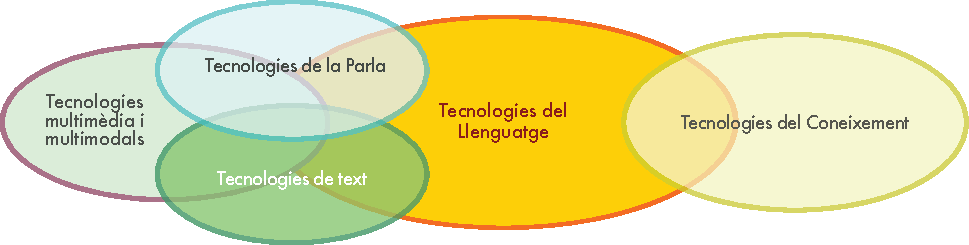
\includegraphics[width=\textwidth]{../_media/catalan/language_technologies}
  \caption{Context de les tecnologies del llenguatge}
  \label{fig:ltincontext_ca}
  \colorrule{grey3}{\textwidth}{1.5pt}
\end{figure*}

Les tecnologies del llenguatge són una àrea establerta de recerca amb un conjunt ampli de literatura introductòria. El lector interessat pot consultar les referències següents: \cite{jurafsky-martin01, manning-schuetze1, lt-world1, lt-survey1}.

Abans de discutir les àrees d'aplicació descrites, descriurem breument l'arquitectura d'un sistema de tecnologies del llenguatge típic.

\subsection[Arquitectures de les aplicacions de tecnologies del llenguatge]{Arquitectures de\newline les aplicacions de tecnologies del llenguatge}

Les aplicacions de programari típiques per al processament de la llengua consisteixen en diversos components que reflecteixen diferents aspectes de la llengua i de la tasca que implementen. La figura \ref{fig:textprocessingarch_ca} mostra una arquitectura molt simplificada tal com la podem trobar en un sistema de processament de text. Els tres primers mòduls tenen a veure amb l’estructura i el significat del text d’entrada:
\begin{itemize}
\item Preprocessat: netejar les dades, eliminar la formatació, detectar la llengua d’entrada, substituir “5è” per “cinquè”, etc.
\item Anàlisi gramatical: trobar el verb i els seus objectes, modificadors, altres elements de l'oració etc.; detectar l’estructura de l’oració.
\item Anàlisi semàntica: desambiguació (quin significat de taula és el correcte donat un context determinat?), resoldre anàfores i expressions de referència com ara ella, el cotxe, etc.; representar el significat de l’oració d’una manera que pugui ser llegible per la màquina.
\end{itemize}


Els mòduls específics per a cada tasca realitzen diferents operacions com ara el resum automàtic d’un text d’entrada, cerques a una base de dades, i moltes d’altres. A continuació iŀlustrem les àrees principals d’aplicació i en destaquem els seus mòduls principals. Una vegada més, les arquitectures de les aplicacions són molt simplificades i idealitzades, per tal d’iŀlustrar la complexitat de les tecnologies del llenguatge d’una manera general i comprensible. Les eines i els recursos més importants involucrats en aquestes arquitectures es troben en negreta en el text i també es poden trobar a la taula al final del capítol. Les seccions on es discuteixen les àrees principals d’aplicació també contenen una descripció general de les indústries actives en aquest camp a Catalunya.

\begin{figure*}[b]
  \colorrule{grey3}{\textwidth}{1.5pt}
  \center
  \vspace{-5mm} 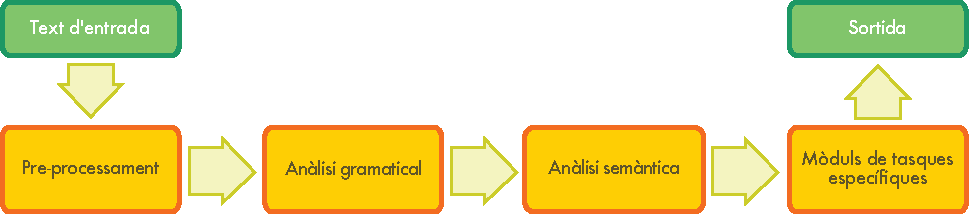
\includegraphics[width=\textwidth]{../_media/catalan/text_processing_app_architecture}
  \caption{Arquitectura típica d'una aplicació de processament de text}
  \label{fig:textprocessingarch_ca}
  \colorrule{grey3}{\textwidth}{1.5pt}
\end{figure*}

Després d’introduir les àrees principals d’aplicació, mostrarem una descripció general de la situació en la recerca i l’educació sobre les tecnologies llenguatge, i conclourem amb un resum dels programes de recerca anteriors i actuals. Al final d’aquesta secció, presentarem un estimació d’experts sobre la situació per que fa a les eines i recursos de les tecnologies del llenguatge bàsiques en funció de dimensions com la disponibilitat, la maduresa o la qualitat. Aquesta taula mostra una bona panoràmica de la situació de les tecnologies del llenguatge per al català.  

\subsection{Àrees principals d’aplicació} 

 En aquesta secció, tractem les eines i els recursos més importants de les tecnologies del llenguatge i 
  donem una visió global de les activitats de les tecnologies del llenguatge a Catalunya. Les eines i recursos en negreta en el text també poden trobar-se a la taula al final d'aquest capítol.

\subsubsection{Correcció d’errors lingüístics}

Qualsevol persona que hagi utilitzat algun processador de textos, com ara el Microsoft Word, haurà vist que aquests programes solen disposar d’una eina que detecta errors ortogràfics i proposa possibles correccions. Quaranta anys després del primer corrector automàtic dissenyat per Ralph Gorin, els programes actuals no es limiten a comparar les paraules utilitzades amb les que conté un diccionari, sinó que fan servir procediments cada cop més sofisticats. A més a més d’incloure algorismes dependents de la llengua que permeten analitzar aspectes morfològics (com per exemple la formació del plural), alguns poden fins i tot reconèixer errors sintàctics, com ara un verb mal conjugat (per exemple, ‘Ella escrius una carta’).

Un corrector lingüístic \ref{fig:langcheckingaarch_ca} d'aquestes prestacions requereix formular les regles gramaticals de cada llengua, una tasca manual que requereix uns grans coneixements sobre la matèria, o bé utilitzar els anomenats models estadístics de la llengua. Aquests models permeten calcular la probabilitat que una paraula concreta aparegui en un determinat entorn (és a dir, les paraules anteriors i posteriors). Per exemple, llibre anglès és una seqüència de paraules molt més probable que no pas llibre anglesa. Un model estadístic es pot obtenir automàticament a partir d’una gran quantitat de dades lingüístiques correctes (és a dir, un corpus). Fins al dia d’avui, aquests mètodes s’han desenvolupat i avaluat principalment en anglès. Malauradament, és difícil transferir-los directament al català, que té una inflexió més rica i un ordre sintàctic de les paraules més flexible.

\begin{figure*}[htb]
  \colorrule{grey3}{\textwidth}{1.5pt}
  \vspace{-9mm}
  \center
  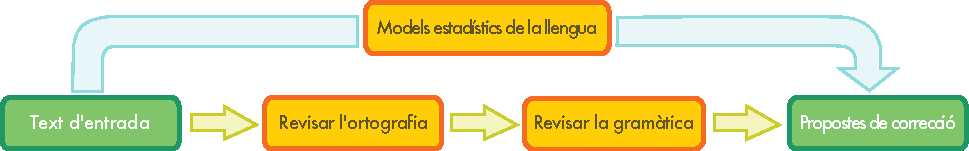
\includegraphics[width=\textwidth]{../_media/catalan/language_checking}
  \caption{Corrector lingüístic (a dalt: estadístic, a baix: basat en regles)}
  \label{fig:langcheckingaarch_ca}
  \colorrule{grey3}{\textwidth}{1.5pt}
\end{figure*}

L’ús d’eines de correcció automàtica no es limita als processadors de textos; també es poden utilitzar com a sistemes de suport per a la creació d’escrits. Degut a l’augment constant de productes tecnològics, la quantitat de documentació tècnica ha crescut ràpidament durant les últimes dècades. Per evitar possibles queixes dels clients per problemes o danys derivats d’una mala comprensió de les instruccions, les empreses han començat a posar més atenció en la qualitat de la documentació tècnica. Els avenços en el processament del llenguatge natural han permès desenvolupar programes de suport que ofereixen ajuda als autors de la documentació i els faciliten la utilització d’un vocabulari i unes estructures d’oracions consistents amb unes determinades regles i restriccions terminològiques (corporatives).

\boxtext{L’ús d’eines de correcció automàtica no es limita als processadors de textos; també es poden utilitzar per a la creació d’escrits}

Només algunes empreses i proveïdors de serveis ofereixen productes en català en aquesta àrea. Enciclopèdia Catalana, Maxigrammar i Inèdit han creat i comercialitzat productes que inclouen la revisió ortogràfica i gramatical per al català, així com eines de revisió adaptades a diversos dominis i estils. Softcatalà i Barcelona Media també han desenvolupat algunes eines lingüístiques que s’ofereixen a la comunitat com a aplicacions web. Una nova versió de “\textit{El corrector}” s’ha desenvolupat i comercialitzat recentment per a Ipod i Ipad. 

A part dels correctors ortogràfics i els programes de suport per a la creació de textos, la revisió dels diferents aspectes lingüístics també és important en l’àmbit dels programes d’ajuda per a l’aprenentatge de llengües, i s’aplica en la correcció automàtica de les cerques enviades als motors de cerca d’Internet (per exemple, en el ‘Volíeu dir:’ de Google). 

\subsubsection{Cerques a la web}

Les cerques a la web, a intranets o a les biblioteques digitals és probablement la tecnologia del llenguatge més utilitzada i, en canvi, la menys desenvolupada de totes. El motor de cerca Google, que es va posar en servei l’any 1998, s’utilitza actualment en aproximadament el 80\% de totes les cerques que es fan arreu del món \cite{CAT-Nota22}. 

Ni la interfície de la cerca ni la presentació dels resultats han canviat de forma significativa des de la primera versió. En la versió actual, Google ofereix la correcció de paraules mal escrites també en català i, des de l’any 2009, ha incorporat informació semàntica bàsica en la seva combinació algorísmica \cite{CAT-Nota23}, que permet millorar la precisió de la cerca analitzant el significat de la consulta segons els seu context. L’èxit de Google mostra que amb una gran quantitat de dades i unes tècniques eficients per indexar-les, es poden obtenir resultats satisfactoris utilitzant principalment mètodes estadístics.

Tot i això, per poder tractar cerques d’informació més sofisticades, és essencial integrar-hi un coneixement lingüístic més profund. En els laboratoris de recerca, per exemple, s’han obtingut millores en diferents experiments utilitzant tesaurus i recursos lingüístics ontològics com el WordNet que permeten trobar resultats a partir de sinònims dels termes de la consulta, o fins i tot termes més llunyans. Com passa gairebé sempre en les tecnologies del llenguatge, aquests mètodes requereixen recursos específics per a cada llengua. En aquesta línia, el centre TALP de la Universitat Politècnica de Catalunya ha desenvolupat un WordNet en català, que es troba disponible de forma gratuïta \cite{CAT-Nota24}. 

La propera generació de motors de cerca haurà d’incloure una tecnologia del llenguatge molt més sofisticada. Si els termes d’una consulta consisteixen en una pregunta o un altre tipus de frase, en comptes d’una simple llista de paraules clau, per proporcionar respostes adequades es requereix una \textbf{anàlisi sintàctica} i semàntica de la consulta, a més  a més de la capacitat de crear un índex que permeti trobar ràpidament els documents rellevants per a la resposta. Per exemple, en el cas que un usuari introdueixi la consulta: ‘Dóna’m una llista de totes les empreses que han estat comprades per altres empreses durant els últims cinc anys’. Per proporcionar una resposta satisfactòria, és necessari aplicar una anàlisi sintàctica per tal d’analitzar l’estructura gramatical de l’oració i poder determinar que el que l’usuari desitja és saber quines empreses han estat comprades per altres, i no quines empreses han comprat altres empreses. A més a més, cal processar  l’expressió ‘durant els últims cinc anys’ per determinar el període al qual fa referència la consulta. 

\begin{figure*}[htb]
  \colorrule{grey3}{\textwidth}{1.5pt}
  \vspace{-9mm}
  \center
  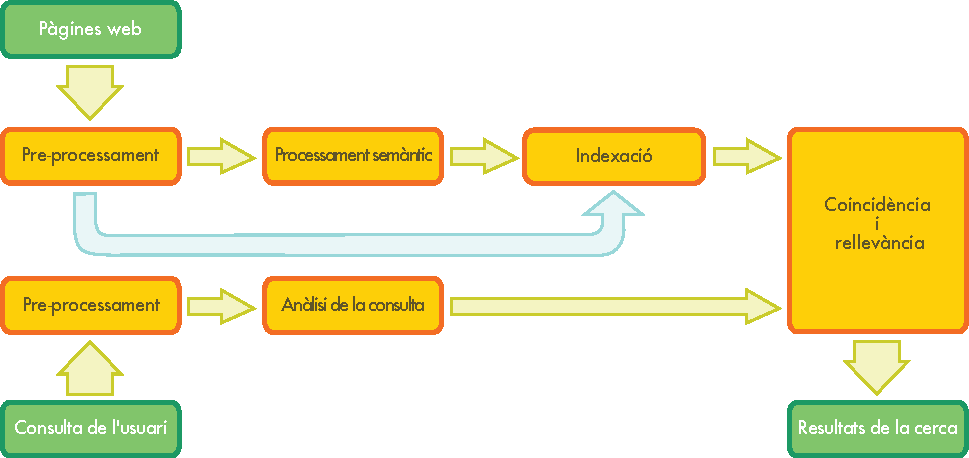
\includegraphics[width=\textwidth]{../_media/catalan/web_search_architecture}
  \vspace{-5mm}
  \caption{Cercador web}
  \label{fig:websearcharch_ca}
  \colorrule{grey3}{\textwidth}{1.5pt}
\end{figure*}

Finalment, la consulta processada s’ha de comparar amb una enorme quantitat de dades no estructurades per tal de trobar la informació que l'usuari està cercant. Aquest procés es coneix habitualment com a ‘recuperació d'informació’ i implica la cerca i la classificació dels documents rellevants. A més a més, per poder generar una llista d’empreses, cal tenir la capacitat de detectar que una cadena determinada de paraules en un document es refereix a un nom d'empresa. Aquest tipus de informació es pot obtenir amb els anomenats reconeixedors de noms d’entitats.

El fet d’intentar trobar la resposta en documents escrits en una llengua diferent de la llengua de consulta és un repte encara més gran. Per fer-lo possible, cal traduir automàticament la consulta a totes les llengües en les quals és possible trobar la resposta, i després traduir la informació trobada a la llengua original. Per altra banda, l’augment de la quantitat d’informació en formats no textuals fa que cada vegada sigui més necessària l’aparició de serveis que permetin cercar informació en entorns multimèdia, és a dir, imatges, àudio i vídeo. El cas de fitxers d’àudio i vídeo implica utilitzar sistemes de \textbf{reconeixement automàtic de la parla} per convertir la veu en un text en el qual es pugui cercar la informació de la consulta. 

Les petites i mitjanes empreses com Inbenta \cite{CAT-inbenta} o RightNow  (anteriorment q-go \cite{CAT-rightnow}) ofereixen motors de cerca amb informació semàntica en català.

\boxtext{La propera generació de motors de cerca haurà d'incloure tecnologies del llenguatge molt més sofisticades.}

També hi ha algunes iniciatives interessants per agrupar motors de cerca específics per al català, com CerCat o Som-hi\cite{CAT-cercadors}. Es pot trobar un resum històric sobre aquest tema a \cite{CAT-Resum-sobre-cercadors}.
  
\subsubsection{Interacció per la parla}

La tecnologia d’interacció per la parla és la base per a la creació d’interfícies que permetin als usuaris interaccionar amb màquines fent servir la veu en comptes d’un teclat, un ratolí o un altre dispositiu. Avui en dia, aquestes interfícies d’usuari orals es fan servir generalment per automatitzar, de forma total o parcial, alguns serveis que les empreses ofereixen als seus clients, treballadors i socis per via telefònica.

Algunes de les àrees empresarials que depenen fortament d’aquest tipus d’interfícies són la banca, la logística, el transport públic i les telecomunicacions. Altres usos d’aquesta tecnologia consisteixen a proporcionar una alternativa a l’entrada i la sortida de dades en determinats dispositius que contenen interfícies d’usuari gràfiques, com ara els sistemes de navegació dels cotxes o els telèfons inteŀligents. 

\begin{figure*}[htb]
  \colorrule{grey3}{\textwidth}{1.5pt}
  \vspace{-9mm}
  \center  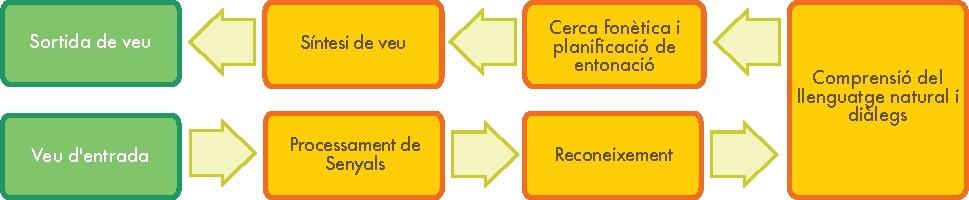
\includegraphics[width=\textwidth]{../_media/catalan/simple_speech-based_dialogue_architecture}
  \center
  \caption{Sistema de diàleg basat en veu}
  \label{fig:dialoguearch_ca}
  \colorrule{grey3}{\textwidth}{1.5pt}
\end{figure*}

En el seu nucli, la interacció mitjançant la parla consta de les quatre tecnologies següents:
\begin{itemize}
\item El \textbf{reconeixement automàtic de la parla} és la part responsable de determinar quines paraules es corresponen amb la seqüència de sons que ha pronunciat l’usuari.
\item L’\textbf{anàlisi sintàctica} i \textbf{interpretació semàntica} s’encarrega d’analitzar sintàcticament les frases que pronuncia l’usuari i d’interpretar el seu significat tenint en compte l’objectiu del sistema.
\item La \textbf{gestió de diàleg} és necessària, en la part en què l’usuari interactua amb el sistema, per determinar quina acció s’ha de dur a terme en funció de la informació que proporciona l’usuari i de les funcions del sistema.
\item La \textbf{síntesi de veu} s’utilitza per transformar un text en sons perquè l’usuari pugui rebre la resposta del sistema en forma de senyal d’àudio. 
\end{itemize}

Un dels reptes més grans és aconseguir tenir un sistema automàtic que reconegui les paraules que pronuncia l’usuari de la manera més precisa possible. Per a això cal o bé restringir el rang de paraules possibles acceptades pel sistema a un conjunt de paraules clau, o bé crear manualment models de la llengua que donin cobertura a un ampli ventall de possibles frases que l’usuari pot pronunciar de forma natural. Mentre la primera opció ofereix una opció força rígida i inflexible que probablement es reflectirà en una baixa acceptació per part dels usuaris, la creació, l’ajust i el manteniment dels models de la llengua pot incrementar significativament els costos. Tot i això, les interfícies orals que fan servir models de la llengua i que permeten que inicialment l’usuari expressi de forma flexible la seva intenció (per exemple, saludant-lo amb un \textit{Com puc ajudar-lo?}) mostren una taxa d’automatització més alta i una acceptació més gran per part dels usuaris, de manera que es poden considerar sistemes avantatjats respecte als mètodes, menys flexibles, de \textit{diàleg dirigit}.

\boxtext{La tecnologia d’interacció mitjançant la parla és la base per a la creació d’interfícies que permetin als usuaris interaccionar amb màquines.}

Per proporcionar una resposta als usuaris dins del marc d’una interfície oral, les empreses tendeixen molt sovint a utilitzar paraules o frases enregistrades per un locutor professional. En casos estàtics, en els quals la pronunciació no depèn del context, aquesta opció proporciona resultats satisfactoris. En canvi, si la pronunciació concreta és important per al missatge, l’experiència de l’usuari es veu molt perjudicada per la pobra prosòdia que resulta de la simple concatenació d’arxius d’àudio. Per reduir aquest problema, els sistemes de síntesi de veu actuals tenen en compte la naturalesa dinàmica de la prosòdia de les frases, i aconsegueixen uns millors, encara que millorables, resultats. 

Pel que fa al mercat de la tecnologia d’interacció per la parla, l’última dècada s’ha caracteritzat per una forta estandardització de les interfícies entre els diferents components, així com dels mètodes per crear programes particulars per a determinades aplicacions. També hi ha hagut una forta consolidació del mercat en els últims deu anys, especialment en el camp del reconeixement de la parla i la síntesi de la veu. Aquí, els mercats nacionals dels països del G20 –és a dir, els països econòmicament forts i amb una població considerable– estan dominats per menys de cincs empreses, essent \textit{Nuance} la més important a Europa, també per al català. Tot i això, algunes empreses locals petites com \textit{Verbio} \cite{CAT-Nota25}, que va sorgir de la Universitat Politècnica de Catalunya i que disposa de la seva pròpia tecnologia, estan començant a competir.

Pel que fa als coneixements i la tecnologia sobre la gestió de diàlegs, els mercats estan fortament dominats per entitats nacionals, les quals són, normalment, petites i mitjanes empreses. 

La majoria d’empreses en el mercat de la síntesi de veu en català són essencialment desenvolupadores d’aplicacions. Les principals dins del mercat espanyol són Indsys \cite{CAT-Nota26} (Intelligent Dialogue Systems), Fonetic \cite{CAT-Nota27}, Ydilo \cite{CAT-Nota28} i NaturalVoz \cite{CAT-Nota29}.

Fent un cop d’ull més enllà de l’estat actual de la tecnologia, en un futur hi haurà canvis significatius degut a la proliferació de telèfons inteŀligents com a noves plataformes per gestionar les relacions amb els clients, a més a més del telèfon, Internet i el correu electrònic. Aquesta tendència també afectarà l’ús de la tecnologia d’interacció per la parla. D’una banda, a llarg termini baixarà la demanda de sistemes telefònics basats en interfícies orals. De l’altra, l’ús de la parla com a interfície amigable per als telèfons inteŀligents guanyarà importància. Aquesta suposició es veu justificada per la millora observable en la precisió dels sistemes de reconeixement de la parla independents del locutor que s’ofereixen actualment com a servei centralitzat per als usuaris de telèfons inteŀligents. Donada aquesta situació, l’ús d’un nucli de tecnologies lingüístiques que sigui específic per a les aplicacions guanyarà importància, suposadament, en comparació amb la situació actual. 

\subsubsection{Traducció automàtica}

La idea de fer servir ordinadors per realitzar traduccions automàtiques va ser proposada per A. D. Booth l’any 1946. A partir d’aleshores, aquesta àrea va disposar de recursos substancials per a la recerca, especialment durant els anys 50 i 80. Malgrat això, la \textbf{traducció automàtica} encara no ha arribat a complir les altes expectatives que va generar en els seus inicis.  

\boxtext{En la seva aproximació més bàsica, la traducció automàtica simplement substitueix cada paraula de la llengua original per la seva equivalent en la llengua objecte.}
\begin{figure*}[htb]
  \colorrule{grey3}{\textwidth}{1.5pt}
  \vspace{-21mm}
  \center
  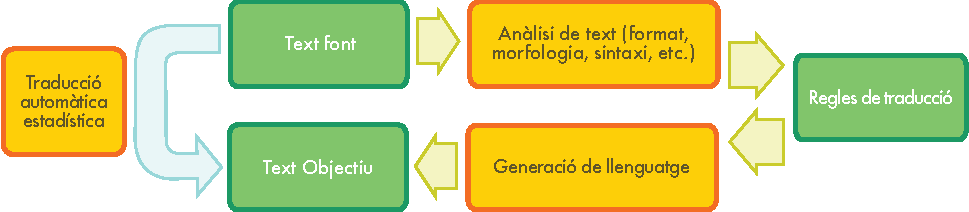
\includegraphics[width=\textwidth]{../_media/catalan/machine_translation}
  \vspace{-2mm}
  \caption{Traducció automàtica (a l'esquerra: estadística, a la dreta: basat en regles)}
  \label{fig:mtarch_ca}
  \colorrule{grey3}{\textwidth}{1.5pt}
\end{figure*}

En la seva aproximació més bàsica, la traducció automàtica simplement substitueix cada paraula de la llengua original per la seva equivalent en la llengua objecte. Aquesta opció pot ser útil en alguns dominis amb un vocabulari molt restringit, com ara els informes meteorològics, o en casos de llengües molt properes. Tot i això, per aconseguir una bona traducció de textos menys estandarditzats, s’han d’analitzar unitats de text més llargues (frases o passatges sencers) per trobar la correspondència més adient en la llengua objecte. La dificultat més gran d’aquest aspecte és que la llengua humana és ambigua, i això implica diversos reptes, com ara trobar el sentit correcte d’una paraula (‘Jaguar’ pot ser un cotxe o un animal, per exemple) o la inclusió de frases preposicionals a un nivell sintàctic, com per exemple:
\begin{itemize}
\item \textit{Passejava amb el nen cantant.}
\item \textit{T1: I was walking with the singer child.}
\item \textit{T2. I was walking and singing with the child.}
\end{itemize}

Una manera d’afrontar aquesta tasca és basar-se en regles lingüístiques. En el cas de llengües molt properes, una traducció directa pot ser viable en casos com els de l’exemple anterior. Però sovint els sistemes basats en regles analitzen el text d’entrada i creen una representació simbòlica intermediària a partir de la qual es genera el text traduït final. L’èxit d’aquests mètodes depèn molt de la disponibilitat d’amplis \textbf{lexica} amb informació morfològica, sintàctica i semàntica, i grans conjunts de \textbf{regles gramaticals} dissenyades amb cura per un lingüista expert.

A partir de finals dels anys 80, a mesura que la capacitat computacional dels ordinadors augmentava i es feia més assequible, l’interès en els models estadístics per a la traducció automàtica va anar creixent. Els paràmetres d’aquests models es calculen a partir de l’anàlisi d’un corpus de textos bilingües, com ara el corpus paraŀlel Europarl, que conté les actes del parlament europeu en vint-i-una llengües europees. Si es disposa de dades suficients, els models estadístics funcionen prou bé com per generar un text traduït que capti el significat aproximant del text original. Tot i així, a diferència dels sistemes basats ens regles, els sistemes basats en models estadístics sovint generen textos gramaticalment incorrectes. D’altra banda, a més de l’avantatge de reduir l’esforç que suposa haver d’escriure les regles gramaticals a mà, els sistemes estadístics poden cobrir particularitats de la llengua que a vegades no apareixen en els sistemes basats en regles, com per exemple les expressions idiomàtiques. 

Com que els punts forts i febles d’aquests dos mètodes són complementaris, gairebé tots el investigadors treballen en sistemes híbrids que els combinen. Això es pot fer de diferents maneres. La primera és utilitzar els dos sistemes, i després triar la millor opció per a cada frase. El problema és que per a frases llargues no hi ha cap resultat que sigui perfecte. Una solució millor és combinar les millors parts de cada frase generada amb diferents sistemes. Aquesta opció és força complexa perquè no sempre resulta obvi quines parts de cada alternativa són les que es corresponen, i per tant, s’han d’alinear.

Degut a la particular situació oficial de bilingüisme existent a les diferents regions d’Espanya i a la similitud entre el català i el castellà, els sistemes de traducció automàtica entre aquestes dues llengües funcionen de forma bastant satisfactòria. Inicialment, alguns dels principals sistemes que es van desenvolupar van ser el METAL (Siemens) i l’ATLAS (Fujitsu). Aquests projectes van tenir lloc a Barcelona durant els anys 90. Al cap d’un temps, les gran empreses que els van impulsar van apartar-se’n, i els projectes van passar a mans de diferents \textit{spin-off}: una empresa local, INCYTA, així com GMS i Lucy Software, la qual és actualment el proveïdor principal de sistemes de traducció en català, van passar a fer-se càrrec de METAL. A més a més, el sistema de traducció entre el català i el castellà que va comprar la Generalitat de Catalunya va passar a ser un servei web públic l’any 2005, mentre que Google va començar a oferir el seu propi sistema l’any 2007.

Altres empreses, com T6 Estàndard Lingüístic i AutomaticTrans, també han desenvolupat sistemes de traducció automàtica. El sistema desenvolupat per AutomaticTrans té el seu origen en la producció d’un diari bilingüe, El Periódico. Actualment hi ha tres diaris disponibles en català i castellà que utilitzen traducció automàtica; els altres dos són El Segre i La Vanguardia. 

La Generalitat Valenciana va promoure la creació del SALT, un sistema de traducció automàtica específic per al valencià. Més recentment, la Universitat Politècnica de València ha tret una versió de SiShiTra, un sistema híbrid. El sistema de codi obert OpenTrad també ofereix una versió en valencià. 

La traducció entre el català i el castellà va ser l’origen de l’Apertium, un sistema de codi obert desenvolupat pel grup Transducens \cite{CAT-transducens} de la Universitat d’Alacant \cite{CAT-UnivAlacant}. L’Apertium és el primer sistema del món basat en tecnologia de traducció automàtica en codi obert, i la seva explotació comercial la duen a terme principalment Prompsit Language Engineering i OpenTrad Consortium. 

La majoria d’aquests sistemes estan basats en regles. Tot i que s’estan fent esforços importants, tant a nivell nacional com internacional, per millorar els sistemes estadístics i híbrids, aquests mètodes encara no proporcionen les mateixes prestacions en aplicacions comercials que en l’àmbit de la recerca. 

Donada una bona adaptació en termes de terminologia específica per l’usuari i una bona integració en el ritme de treball, l’ús de la traducció automàtica pot incrementar la productivitat significativament. Així, des de començaments del segle XXI, el principal usuari d’aquests sistemes en català és l’administració pública, inclosos alguns departaments del govern com el de justícia.

Es considera que la qualitat dels sistemes de traducció encara té un gran marge de millora. Alguns dels principals reptes són aconseguir adaptar els recursos lingüístics a un determinat domini i la integració en processos de treballs existents amb bases terminològiques i memòries de traducció.

A més a més, la majoria de corpus paraŀlels existents són entre el català i el castellà, de manera que en la majoria de traductors per al català, el castellà és la llengua pivot.

\begin{figure*}[tb]
  \centering
  \setlength{\tabcolsep}{0.17em}
  \small
  \begin{tabular}{>{\columncolor{corange1}}cccccccccccccccccccccccc}
    & \multicolumn{22}{>{\columncolor{corange1}}c}{Target language -- \textcolor{grey1}{Target language}}\\\addlinespace[{-.009cm}]
    \rowcolor{corange1}  & EN & BG & DE & CS & DA & EL & ES & ET & FI & FR & HU & IT & LT & LV & MT & NL & PL & PT & RO & SK & SL & SV\\
    EN & -- & \textcolor{blue}{40.5} & \textcolor{blue}{46.8} & \textcolor{green2}{52.6} & \textcolor{green2}{50.0} & \textcolor{blue}{41.0} & \textcolor{green2}{55.2} & \textcolor{purple}{34.8} & \textcolor{purple}{38.6} & \textcolor{green2}{50.1} & \textcolor{purple}{37.2} & \textcolor{green2}{50.4} & \textcolor{purple}{39.6} & \textcolor{blue}{43.4} & \textcolor{purple}{39.8} & \textcolor{green2}{52.3} & \textcolor{blue}{49.2} & \textcolor{green2}{55.0} & \textcolor{blue}{49.0} & \textcolor{blue}{44.7} & \textcolor{green2}{50.7} & \textcolor{green2}{52.0}\\
    BG & \textcolor{green}{61.3} & -- & \textcolor{purple}{38.7} & \textcolor{purple}{39.4} & \textcolor{purple}{39.6} & \textcolor{purple}{34.5} & \textcolor{blue}{46.9} & \textcolor{red3}{25.5} & \textcolor{red3}{26.7} & \textcolor{blue}{42.4} & \textcolor{red3}{22.0} & \textcolor{blue}{43.5} & \textcolor{red3}{29.3} & \textcolor{red3}{29.1} & \textcolor{red3}{25.9} & \textcolor{blue}{44.9} & \textcolor{purple}{35.1} & \textcolor{blue}{45.9} & \textcolor{purple}{36.8} & \textcolor{purple}{34.1} & \textcolor{purple}{34.1} & \textcolor{purple}{39.9}\\
    DE & \textcolor{green2}{53.6} & \textcolor{red3}{26.3} & -- & \textcolor{purple}{35.4} & \textcolor{blue}{43.1} & \textcolor{purple}{32.8} & \textcolor{blue}{47.1} & \textcolor{red3}{26.7} & \textcolor{red3}{29.5} & \textcolor{purple}{39.4} & \textcolor{red3}{27.6} & \textcolor{blue}{42.7} & \textcolor{red3}{27.6} & \textcolor{purple}{30.3} & \textcolor{red2}{19.8} & \textcolor{green2}{50.2} & \textcolor{purple}{30.2} & \textcolor{blue}{44.1} & \textcolor{purple}{30.7} & \textcolor{red3}{29.4} & \textcolor{purple}{31.4} & \textcolor{blue}{41.2}\\
    CS & \textcolor{green2}{58.4} & \textcolor{purple}{32.0} & \textcolor{blue}{42.6} & -- & \textcolor{blue}{43.6} & \textcolor{purple}{34.6} & \textcolor{blue}{48.9} & \textcolor{purple}{30.7} & \textcolor{purple}{30.5} & \textcolor{blue}{41.6} & \textcolor{red3}{27.4} & \textcolor{blue}{44.3} & \textcolor{purple}{34.5} & \textcolor{purple}{35.8} & \textcolor{red3}{26.3} & \textcolor{blue}{46.5} & \textcolor{purple}{39.2} & \textcolor{blue}{45.7} & \textcolor{purple}{36.5} & \textcolor{blue}{43.6} & \textcolor{blue}{41.3} & \textcolor{blue}{42.9}\\
    DA & \textcolor{green2}{57.6} & \textcolor{red3}{28.7} & \textcolor{blue}{44.1} & \textcolor{purple}{35.7} & -- & \textcolor{purple}{34.3} & \textcolor{blue}{47.5} & \textcolor{red3}{27.8} & \textcolor{purple}{31.6} & \textcolor{blue}{41.3} & \textcolor{red3}{24.2} & \textcolor{blue}{43.8} & \textcolor{red3}{29.7} & \textcolor{purple}{32.9} & \textcolor{red3}{21.1} & \textcolor{blue}{48.5} & \textcolor{purple}{34.3} & \textcolor{blue}{45.4} & \textcolor{purple}{33.9} & \textcolor{purple}{33.0} & \textcolor{purple}{36.2} & \textcolor{blue}{47.2}\\
    EL & \textcolor{green2}{59.5} & \textcolor{purple}{32.4} & \textcolor{blue}{43.1} & \textcolor{purple}{37.7} & \textcolor{blue}{44.5} & -- & \textcolor{green2}{54.0} & \textcolor{red3}{26.5} & \textcolor{red3}{29.0} & \textcolor{blue}{48.3} & \textcolor{red3}{23.7} & \textcolor{blue}{49.6} & \textcolor{red3}{29.0} & \textcolor{purple}{32.6} & \textcolor{red3}{23.8} & \textcolor{blue}{48.9} & \textcolor{purple}{34.2} & \textcolor{green2}{52.5} & \textcolor{purple}{37.2} & \textcolor{purple}{33.1} & \textcolor{purple}{36.3} & \textcolor{blue}{43.3}\\
    ES & \textcolor{green}{60.0} & \textcolor{purple}{31.1} & \textcolor{blue}{42.7} & \textcolor{purple}{37.5} & \textcolor{blue}{44.4} & \textcolor{purple}{39.4} & -- & \textcolor{red3}{25.4} & \textcolor{red3}{28.5} & \textcolor{green2}{51.3} & \textcolor{red3}{24.0} & \textcolor{green2}{51.7} & \textcolor{red3}{26.8} & \textcolor{purple}{30.5} & \textcolor{red3}{24.6} & \textcolor{blue}{48.8} & \textcolor{purple}{33.9} & \textcolor{green2}{57.3} & \textcolor{purple}{38.1} & \textcolor{purple}{31.7} & \textcolor{purple}{33.9} & \textcolor{blue}{43.7}\\
    ET & \textcolor{green2}{52.0} & \textcolor{red3}{24.6} & \textcolor{purple}{37.3} & \textcolor{purple}{35.2} & \textcolor{purple}{37.8} & \textcolor{red3}{28.2} & \textcolor{blue}{40.4} & -- & \textcolor{purple}{37.7} & \textcolor{purple}{33.4} & \textcolor{purple}{30.9} & \textcolor{purple}{37.0} & \textcolor{purple}{35.0} & \textcolor{purple}{36.9} & \textcolor{red3}{20.5} & \textcolor{blue}{41.3} & \textcolor{purple}{32.0} & \textcolor{purple}{37.8} & \textcolor{red3}{28.0} & \textcolor{purple}{30.6} & \textcolor{purple}{32.9} & \textcolor{purple}{37.3}\\
    FI & \textcolor{blue}{49.3} & \textcolor{red3}{23.2} & \textcolor{purple}{36.0} & \textcolor{purple}{32.0} & \textcolor{purple}{37.9} & \textcolor{red3}{27.2} & \textcolor{purple}{39.7} & \textcolor{purple}{34.9} & -- & \textcolor{red3}{29.5} & \textcolor{red3}{27.2} & \textcolor{purple}{36.6} & \textcolor{purple}{30.5} & \textcolor{purple}{32.5} & \textcolor{red2}{19.4} & \textcolor{blue}{40.6} & \textcolor{red3}{28.8} & \textcolor{purple}{37.5} & \textcolor{red3}{26.5} & \textcolor{red3}{27.3} & \textcolor{red3}{28.2} & \textcolor{purple}{37.6}\\
    FR & \textcolor{green}{64.0} & \textcolor{purple}{34.5} & \textcolor{blue}{45.1} & \textcolor{purple}{39.5} & \textcolor{blue}{47.4} & \textcolor{blue}{42.8} & \textcolor{green}{60.9} & \textcolor{red3}{26.7} & \textcolor{purple}{30.0} & -- & \textcolor{red3}{25.5} & \textcolor{green2}{56.1} & \textcolor{red3}{28.3} & \textcolor{purple}{31.9} & \textcolor{red3}{25.3} & \textcolor{green2}{51.6} & \textcolor{purple}{35.7} & \textcolor{green}{61.0} & \textcolor{blue}{43.8} & \textcolor{purple}{33.1} & \textcolor{purple}{35.6} & \textcolor{blue}{45.8}\\
    HU & \textcolor{blue}{48.0} & \textcolor{red3}{24.7} & \textcolor{purple}{34.3} & \textcolor{purple}{30.0} & \textcolor{purple}{33.0} & \textcolor{red3}{25.5} & \textcolor{purple}{34.1} & \textcolor{red3}{29.6} & \textcolor{red3}{29.4} & \textcolor{purple}{30.7} & -- & \textcolor{purple}{33.5} & \textcolor{red3}{29.6} & \textcolor{purple}{31.9} & \textcolor{red2}{18.1} & \textcolor{purple}{36.1} & \textcolor{red3}{29.8} & \textcolor{purple}{34.2} & \textcolor{red3}{25.7} & \textcolor{red3}{25.6} & \textcolor{red3}{28.2} & \textcolor{purple}{30.5}\\
    IT & \textcolor{green}{61.0} & \textcolor{purple}{32.1} & \textcolor{blue}{44.3} & \textcolor{purple}{38.9} & \textcolor{blue}{45.8} & \textcolor{blue}{40.6} & \textcolor{red3}{26.9} & \textcolor{red3}{25.0} & \textcolor{red3}{29.7} & \textcolor{green2}{52.7} & \textcolor{red3}{24.2} & -- & \textcolor{red3}{29.4} & \textcolor{purple}{32.6} & \textcolor{red3}{24.6} & \textcolor{green2}{50.5} & \textcolor{purple}{35.2} & \textcolor{green2}{56.5} & \textcolor{purple}{39.3} & \textcolor{purple}{32.5} & \textcolor{purple}{34.7} & \textcolor{blue}{44.3}\\
    LT & \textcolor{green2}{51.8} & \textcolor{red3}{27.6} & \textcolor{purple}{33.9} & \textcolor{purple}{37.0} & \textcolor{purple}{36.8} & \textcolor{red3}{26.5} & \textcolor{red3}{21.1} & \textcolor{purple}{34.2} & \textcolor{purple}{32.0} & \textcolor{purple}{34.4} & \textcolor{red3}{28.5} & \textcolor{purple}{36.8} & -- & \textcolor{blue}{40.1} & \textcolor{red3}{22.2} & \textcolor{purple}{38.1} & \textcolor{purple}{31.6} & \textcolor{purple}{31.6} & \textcolor{red3}{29.3} & \textcolor{purple}{31.8} & \textcolor{purple}{35.3} & \textcolor{purple}{35.3}\\
    LV & \textcolor{green2}{54.0} & \textcolor{red3}{29.1} & \textcolor{purple}{35.0} & \textcolor{purple}{37.8} & \textcolor{purple}{38.5} & \textcolor{red3}{29.7} & \textcolor{red2}{8.0} & \textcolor{purple}{34.2} & \textcolor{purple}{32.4} & \textcolor{purple}{35.6} & \textcolor{red3}{29.3} & \textcolor{purple}{38.9} & \textcolor{purple}{38.4} & -- & \textcolor{red3}{23.3} & \textcolor{blue}{41.5} & \textcolor{purple}{34.4} & \textcolor{purple}{39.6} & \textcolor{purple}{31.0} & \textcolor{purple}{33.3} & \textcolor{purple}{37.1} & \textcolor{purple}{38.0}\\
    MT & \textcolor{green}{72.1} & \textcolor{purple}{32.2} & \textcolor{purple}{37.2} & \textcolor{purple}{37.9} & \textcolor{purple}{38.9} & \textcolor{purple}{33.7} & \textcolor{blue}{48.7} & \textcolor{red3}{26.9} & \textcolor{red3}{25.8} & \textcolor{blue}{42.4} & \textcolor{red3}{22.4} & \textcolor{blue}{43.7} & \textcolor{purple}{30.2} & \textcolor{purple}{33.2} & -- & \textcolor{blue}{44.0} & \textcolor{purple}{37.1} & \textcolor{blue}{45.9} & \textcolor{purple}{38.9} & \textcolor{purple}{35.8} & \textcolor{blue}{40.0} & \textcolor{blue}{41.6}\\
    NL & \textcolor{green2}{56.9} & \textcolor{red3}{29.3} & \textcolor{blue}{46.9} & \textcolor{purple}{37.0} & \textcolor{blue}{45.4} & \textcolor{purple}{35.3} & \textcolor{blue}{49.7} & \textcolor{red3}{27.5} & \textcolor{red3}{29.8} & \textcolor{blue}{43.4} & \textcolor{red3}{25.3} & \textcolor{blue}{44.5} & \textcolor{red3}{28.6} & \textcolor{purple}{31.7} & \textcolor{red3}{22.0} & -- & \textcolor{purple}{32.0} & \textcolor{blue}{47.7} & \textcolor{purple}{33.0} & \textcolor{purple}{30.1} & \textcolor{purple}{34.6} & \textcolor{blue}{43.6}\\
    PL & \textcolor{green}{60.8} & \textcolor{purple}{31.5} & \textcolor{blue}{40.2} & \textcolor{blue}{44.2} & \textcolor{blue}{42.1} & \textcolor{purple}{34.2} & \textcolor{blue}{46.2} & \textcolor{red3}{29.2} & \textcolor{red3}{29.0} & \textcolor{blue}{40.0} & \textcolor{red3}{24.5} & \textcolor{blue}{43.2} & \textcolor{purple}{33.2} & \textcolor{purple}{35.6} & \textcolor{red3}{27.9} & \textcolor{blue}{44.8} & -- & \textcolor{blue}{44.1} & \textcolor{purple}{38.2} & \textcolor{purple}{38.2} & \textcolor{purple}{39.8} & \textcolor{blue}{42.1}\\
    PT & \textcolor{green}{60.7} & \textcolor{purple}{31.4} & \textcolor{blue}{42.9} & \textcolor{purple}{38.4} & \textcolor{blue}{42.8} & \textcolor{blue}{40.2} & \textcolor{green}{60.7} & \textcolor{red3}{26.4} & \textcolor{red3}{29.2} & \textcolor{green2}{53.2} & \textcolor{red3}{23.8} & \textcolor{green2}{52.8} & \textcolor{red3}{28.0} & \textcolor{purple}{31.5} & \textcolor{red3}{24.8} & \textcolor{blue}{49.3} & \textcolor{purple}{34.5} & -- & \textcolor{purple}{39.4} & \textcolor{purple}{32.1} & \textcolor{purple}{34.4} & \textcolor{blue}{43.9}\\
    RO & \textcolor{green}{60.8} & \textcolor{purple}{33.1} & \textcolor{purple}{38.5} & \textcolor{purple}{37.8} & \textcolor{blue}{40.3} & \textcolor{purple}{35.6} & \textcolor{green2}{50.4} & \textcolor{red3}{24.6} & \textcolor{red3}{26.2} & \textcolor{blue}{46.5} & \textcolor{red3}{25.0} & \textcolor{blue}{44.8} & \textcolor{red3}{28.4} & \textcolor{red3}{29.9} & \textcolor{red3}{28.7} & \textcolor{blue}{43.0} & \textcolor{purple}{35.8} & \textcolor{blue}{48.5} & -- & \textcolor{purple}{31.5} & \textcolor{purple}{35.1} & \textcolor{purple}{39.4}\\
    SK & \textcolor{green}{60.8} & \textcolor{purple}{32.6} & \textcolor{purple}{39.4} & \textcolor{blue}{48.1} & \textcolor{blue}{41.0} & \textcolor{purple}{33.3} & \textcolor{blue}{46.2} & \textcolor{red3}{29.8} & \textcolor{red3}{28.4} & \textcolor{purple}{39.4} & \textcolor{red3}{27.4} & \textcolor{blue}{41.8} & \textcolor{purple}{33.8} & \textcolor{purple}{36.7} & \textcolor{red3}{28.5} & \textcolor{blue}{44.4} & \textcolor{purple}{39.0} & \textcolor{blue}{43.3} & \textcolor{purple}{35.3} & -- & \textcolor{blue}{42.6} & \textcolor{blue}{41.8}\\
    SL & \textcolor{green}{61.0} & \textcolor{purple}{33.1} & \textcolor{purple}{37.9} & \textcolor{blue}{43.5} & \textcolor{blue}{42.6} & \textcolor{purple}{34.0} & \textcolor{blue}{47.0} & \textcolor{purple}{31.1} & \textcolor{red3}{28.8} & \textcolor{purple}{38.2} & \textcolor{red3}{25.7} & \textcolor{blue}{42.3} & \textcolor{purple}{34.6} & \textcolor{purple}{37.3} & \textcolor{purple}{30.0} & \textcolor{blue}{45.9} & \textcolor{purple}{38.2} & \textcolor{blue}{44.1} & \textcolor{purple}{35.8} & \textcolor{purple}{38.9} & -- & \textcolor{blue}{42.7}\\
    SV & \textcolor{green2}{58.5} & \textcolor{red3}{26.9} & \textcolor{blue}{41.0} & \textcolor{purple}{35.6} & \textcolor{blue}{46.6} & \textcolor{purple}{33.3} & \textcolor{blue}{46.6} & \textcolor{red3}{27.4} & \textcolor{purple}{30.9} & \textcolor{purple}{38.9} & \textcolor{red3}{22.7} & \textcolor{blue}{42.0} & \textcolor{red3}{28.2} & \textcolor{purple}{31.0} & \textcolor{red3}{23.7} & \textcolor{blue}{45.6} & \textcolor{purple}{32.2} & \textcolor{blue}{44.2} & \textcolor{purple}{32.7} & \textcolor{purple}{31.3} & \textcolor{purple}{33.5} & --\\
    \end{tabular}
  \caption{Traducció automàtica entre 22 llengües europees -- \textcolor{grey1}{Machine translation between 22 EU-languages \cite{euro1}}}
  \label{fig:euromatrix_en}
\end{figure*}

Les campanyes avaluadores ajuden a comparar la qualitat dels sistemes de traducció automàtica, les seves aproximacions i l'estat dels sistemes per diferents parelles d'idiomes. La figura~\ref{fig:euromatrix_en} (p.~\pageref{fig:euromatrix_en}), que es va preparar durant el projecte Euromatrix+, mostra les actuacions per parelles obtingudes per 22 dels 23 idiomes de la Unió Europea (L'irlandès no va comparar-se). Els resultats s'ordenen d'acord a una puntuació BLEU, que indica més altes puntuacions per millors traduccions \cite{bleu1}. Un traductor humà aconseguiria normalment al voltant de 80 punts. Els millors resultats (en verd i blau) van ser aconseguits per idiomes que es beneficien d'un esforç de recerca considerable en programes coordinats i en l'existència de molts còrpora paral·lels (p. ex: anglès, francès, holandès, espanyol i alemany). Els idiomes amb els resultats més pobres es mostren en vermell. A aquests els manquen els esforços de desenvolupament mencionats o són estructuralment molt diferents dels altres idiomes (p. ex: hongarès, maltès, finès)

\subsection{Altres àrees d'aplicació}

Desenvolupar aplicacions que utilitzin tecnologies del llenguatge implica una sèrie de tasques que no sempre són visibles per l’usuari final, però que proporcionen funcions importants per al sistema. Per tant, la recerca és important en aquestes àrees, les quals han esdevingut disciplines especialitzades dins de la lingüística computacional.

La cerca automàtica de respostes, tasca coneguda habitualment com a \textit{question answering} (QA), s’ha convertit en una àrea d’investigació molt activa. Per aquest motiu, s’han construït diversos corpus degudament etiquetats i s’han posat en marxa competicions científiques. L’objectiu és passar de les consultes actuals basades en paraules clau (a les quals el motor de cerca respon amb una coŀlecció de documents potencialment rellevants) a un escenari on l’usuari pugui fer una pregunta concreta i rebre del sistema una sola resposta. Per exemple, es podria preguntar: ‘A quina edat va anar Neil Armstrong a la Lluna?’. I la resposta seria ‘38’. Tot i que aquesta tasca està evidentment relacionada amb la cerca d’informació a la web mencionada anteriorment, el terme QA s’utilitza actualment per referir-se a qüestions com el tipus de consultes que s’haurien de distingir i com s’han de tractar, com es pot analitzar un conjunt de documents que contenen potencialment la resposta cercada, i com es pot extreure la resposta d’un document de forma eficient sense deixar excessivament de banda el context.

A la vegada, tot això també està relacionat amb l’extracció d’informació, una àrea que va gaudir de molta popularitat i influència durant el principi dels anys 90, quan la lingüística computacional va començar a fer ús de mètodes estadístics. L’objectiu de l’extracció d’informació és identificar fragments específics d’informació dins de determinades classes de documents; per exemple, detectar els principals participants en compres de companyies segons les notícies aparegudes als diaris. Una altra aplicació possible és analitzar els informes sobre atemptats terroristes per extreure’n els autors, els objectius, la data i la localització de l’atemptat i els seus resultats. El fet d’haver d’analitzar textos i omplir unes plantilles que tenen un format específic del domini de la tasca concreta és una de les característiques habituals de l’extracció d’informació. Aquesta tasca és, per tant, un altre exemple de tecnologies que no són directament visibles per l’usuari perquè queden integrades en les aplicacions, però que tot i així constitueixen una àrea de recerca ben marcada.

\boxtext{Les aplicacions de les tecnologies del llenguatge proporcionen serveis i funcions importants per al sistema poc perceptibles per l'usuari final.}

Hi ha dues tasques, la generació i el resum de textos, que es troben al límit entre dues àrees de recerca, ja que a vegades poden ser útils directament per si soles i altres s’utilitzen com a part d’aplicacions més grans. El resum de textos es refereix, evidentment, a la tasca de crear una versió curta d’un text més llarg i s’ofereix, per exemple, com a funció dins del MS Word. Funciona principalment utilitzant mètodes estadístics, identificant primer les paraules més rellevants (que poden ser, per exemple, paraules molt freqüents en el text, però que no ho són en general) per després determinar les frases que contenen més paraules importants. Aquestes frases es marquen en el document, o s’extreuen d’ell, i s’utilitzen per construir el resum. Amb aquest mètode, que és el més utilitzat amb diferència, el resum es redueix a l’extracció d’un conjunt de frases del text principal. Tots els programes comercials que fan resums automàtics utilitzen aquesta idea. Una alternativa, sobre la qual s’està treballant, és crear noves frases que no tenen per què aparèixer en el text original. Això requereix una comprensió més profunda del text i, per tant, és una opció molt menys robusta. En qualsevol cas, la generació de textos generalment no s’utilitza per si sola, sinó que forma part d’aplicacions més grans, com ara un sistema d’informació clínica que recull, emmagatzema i processa dades dels pacients, del qual la generació d’informes n’és només una part. 

\boxtext{Pel català, com per a la majoria de llengües, la recerca a la majoria de llengues, la recerca de les tecnologies del llenguatge es troba molt menys desenvolupada que per l'anglès.}

La situació actual en aquestes àrees de recerca per a la majoria de llengües es troba en un estat molt menys avançat que per a l’anglès, llengua per a la qual s’han organitzat nombroses competicions, especialment pel DARPA/NIST als Estats Units. Aquest fet ha ajudat a millorar les prestacions d’aquestes tecnologies, però principalment en anglès. També s’han fet algunes competicions en vàries llengües, però el català mai s’ha tingut gaire en compte. En conseqüència, hi ha molt pocs corpus anotats o altres recursos per a aquestes tasques. Els sistemes de resum, quan utilitzen únicament mètodes estadístics, es poden utilitzar sovint independentment de la llengua, i això ha facilitat l’existència d’alguns prototips disponibles. En el cas de la generació de text, alguns components dels sistemes en anglès es poden aprofitar, però no tots. 

\subsection{Les tecnologies del llenguatge a l’educació}

Les tecnologies del llenguatge és un camp que involucra experts de moltes disciplines diferents com ara lingüistes, informàtics, matemàtics, filòsofs i neurocientífics, entre d’altres. Tot i que aquesta àrea de recerca encara no ocupa un lloc fix en cap universitat de l’àmbit català, és a Barcelona on es concentren la majoria de projectes. 
Actualment hi ha diversos graus relacionats amb les tecnologies del llenguatge disponibles en algunes universitats, com la Universitat d’Alacant, la Universitat de Barcelona, la Universitat Pompeu Fabra o la Universitat Oberta de Catalunya.
Pel que fa a màsters i postgraus, la Universitat Autònoma de Barcelona ofereix el Màster internacional en processament del llenguatge natural i tecnologies del llenguatge, en coŀlaboració amb universitats estrangeres. A part d’això, existeixen altres màsters en els quals el processament del llenguatge natural és una de les àrees que s’estudien (per exemple a la Universitat de Barcelona, la Universitat Pompeu Fabra, la Universitat de Girona, la Universitat Rovira i Virgili, la Universitat d’Alacant, la Universitat de Castelló i la Universitat Politècnica de València). 
També hi ha programes de doctorat en els quals les tecnologies del llenguatge  és una de les àrees de recerca (com per exemple a la Universitat d’Alacant, a la Universitat de Barcelona i a la Universitat Rovira i Virgili).

\subsection{Programes de suport per a les tecnologies del llenguatge}

Tant el govern català com l’espanyol han donat suport a les tecnologies del llenguatge a través de diferents programes. 

L’existència d’una important activitat, especialment a Barcelona, en l’àmbit de les tecnologies del llenguatge es pot entendre a través dels programes de suport i projectes de recerca que s’han dut a terme en les últimes dècades. Un dels primers programes va ser EUROTRA, un ambiciós projecte sobre traducció automàtica fundat per la Comissió Europea, que va tenir lloc entre finals dels anys 70 i l’any 1994. Encara que EUROTRA no va treballar en el català, aquest projecte, que va tenir un gran impacte en la industria de la llengua a Europa, va ser crucial per remarcar la importància de les llengües en el món de la tecnologia, i de quina manera podria afectar l’evolució tecnològica a les llengües petites i mitjanes. El govern català va entendre de seguida el repte que això implicava i va posar en marxa diversos programes per, bàsicament, localitzar diferents eines informàtiques. 

La Generalitat de Catalunya ha donat suport durant més de vint anys a la recerca i el desenvolupament comercial de tecnologies de traducció automàtica, reconeixement de la parla i correcció ortogràfica i gramatical. La Secretaria de Política Lingüística, el Comissionat per a la Societat de la Informació i la Secretaria de Telecomunicacions i Societat de la Informació han estat els motors principals de les polítiques de suport. A més a més, la traducció automàtica en català s’ha beneficiat de programes de suport del govern espanyol. Projectes com l’Apertium (un sistema de traducció en codi obert) i OpenTrad, així com altres projectes petits, han rebut finançament per part del Ministeri de Ciència i Tecnologia. 

El CREL (Centre de Referència en Enginyeria Lingüística, 1996-2000), gestionat per l’Institut d’Estudis Catalans amb la participació de les principals Universitats Catalanes, es va crear amb l’objectiu específic de promoure la creació d’eines i recursos pel processament automàtic de textos en català en diverses aplicacions. 

Pel que fa a la presència del català en els projectes europeus, l’any 2008 el govern català va signar un acord amb la Universitat Pompeu Fabra, el representant nacional en el projecte europeu CLARIN, per construir un sistema de demostració. L’objectiu principal d’aquest sistema (CLARIN-CAT-LAB), que està disponible per a la recerca \cite{CAT-Nota30}, és integrar recursos i tecnologia en català per garantir la presència d’aquesta llengua en la infraestructura resultant del projecte CLARIN. A més a més, la Biblioteca de Catalunya, juntament amb altres institucions catalanes, és un dels participants del projecte EUROPEANA. 

Des de l’any 2000 fins ara, el govern espanyol ha donat suport, dins del pla nacional de recerca i tecnologia, a diversos projectes en l’àrea de les tecnologies de la parla multilingüe: TEHAM, AVIVAVOZ i BUCEADOR. El principal objectiu d’aquests projectes és augmentar les prestacions dels sistemes de reconeixement de la parla, traducció i síntesi de veu en totes les llengües oficials a Espanya: basc, gallec, català i castellà. 

L’any 2005, el govern català va posar en marxa un projecte per generar recursos lingüístics pel reconeixement de la parla i la síntesi de veu. Més tard, el projecte TECNOPARLA (2007-2010) es va crear per traduir veu entre el català i el castellà. Els senyals de veu es van obtenir a partir de programes de televisió. D’aquest projecte en van resultar molts avenços en diferents tecnologies: reconeixement de la parla, traducció automàtica i síntesi de veu.

\subsection{Eines i recursos disponibles}

La següent taula proporciona un resum de la situació actual de les tecnologies del llenguatge en català. La puntuació sobre els recursos i les eines existents està basat en les estimacions de diferents experts basant-se en una escala del 0 (molt baixa) a 6 (molt alta) d'acord amb set criteris.

\begin{figure*}[htb]
  \centering
\begin{tabular}{>{\columncolor{orange1}}p{.33\linewidth}@{\hspace*{6mm}}c@{\hspace*{6mm}}c@{\hspace*{6mm}}c@{\hspace*{6mm}}c@{\hspace*{6mm}}c@{\hspace*{6mm}}c@{\hspace*{6mm}}c}
\rowcolor{orange1}
 \cellcolor{white}&
 \begin{sideways}\makecell[l]{Quantitat}\end{sideways} &
 \begin{sideways}\makecell[l]{\makecell[l]{Disponibilitat} }\end{sideways} &
 \begin{sideways}\makecell[l]{Qualitat}\end{sideways} &
 \begin{sideways}\makecell[l]{Cobertura}\end{sideways} &
 \begin{sideways}\makecell[l]{Maduresa}\end{sideways} &
 \begin{sideways}\makecell[l]{Sostenibilitat}\end{sideways} &
 \begin{sideways}\makecell[l]{Adaptabilitat}\end{sideways} \\ \addlinespace

\multicolumn{8}{>{\columncolor{orange2}}l}{\textcolor{black}{Tecnologies del llenguatge: eines, tecnologies i aplicacions}} \\ \addlinespace

Reconeixement de la parla	&3&3&3&3&3&3&2 \\ \addlinespace
Síntesi de veu &4&2&4&4&5&4&2\\ \addlinespace
Anàlisi gramatical &3&2.5&4&4&4&2.5&2.5\\ \addlinespace
Anàlisi semàntic &1&1&2&1&1&1&1\\ \addlinespace
Generació de text &1&2&3&1&3&3&1\\ \addlinespace
Traducció automàtica &3&3&2&3&4&1&2\\ \addlinespace

\multicolumn{8}{>{\columncolor{orange2}}l}{\textcolor{black}{Recursos lingüístics: recursos, dades, bases de coneixement}} \\ \addlinespace

Corpora textuals &3&2.5&3.5&3&3&2.5&2.5\\ \addlinespace
Corpora orals &3&5&3&2&3&3&2\\ \addlinespace
Corpora paraŀlels &2&1&2&2&2&1&1\\ \addlinespace
Recursos lèxics &2.5&2&3&2.5&3&3&2.5\\ \addlinespace
Gramàtiques &2&3&2&2&2&2&2\\
\end{tabular}
 \caption{Estat del suport a les tecnologies del llenguatge pel Català}
 \label{tab:lrlttable}
\end{figure*}

La taula es pot resumir amb els següents punts clau, que remarquen els aspectes més importants per poder millorar les tecnologies actuals del processament automàtic del català:
\begin{itemize}
\item Tot i que existeixen alguns corpus específics de gran qualitat, encara manquen corpus grans amb anotacions sintàctiques i semàntiques. 
\item Hi ha un corpus de referència del català, però aconseguir-lo per a desenvolupaments tecnològics no és fàcil ni econòmic.
\item La majoria de recursos no compleixen cap estàndard. Per tant, es necessiten iniciatives per estandarditzar les dades i transformar formats. 
\item La semàntica és més difícil de processar que la sintaxi. I la semàntica dels textos llargs és més complexa d’analitzar que la de les paraules o les frases. 
\item Quan una determinada eina té en compte aspectes semàntics, es fa més difícil trobar les dades adients i suficientes per treballar amb mètodes estadístics. Per tant, es necessari aprofondir en els coneixements per poder desenvolupar processament que dugui a la comprensió del text. 
\item Existeixen estàndards per la semàntica a nivell de paraula (RDF, OWL, etc.); tot i així, no és senzill aplicar-los a tasques de processament del llenguatge natural. 
\item Actualment, el processament de la parla es troba en una fase més madura que el processament del llenguatge natural de textos escrits. 
\item Hi ha molts grups que treballen en traducció automàtica, especialment entre el català i el castellà.
\item  S’ha aconseguit dissenyar amb èxit aplicacions particulars d’alta qualitat, però és pràcticament impossible proposar solucions estandarditzades donada la situació actual relativa al finançament.
\end{itemize}

\subsection{Comparació entre llengües}

L'estat actual del suport a les tecnologies de llenguatge varia considerablement d'una comunitat lingüística a una altra. Per tal de comparar la situació entre llengües, aquesta secció presentarà una avaluació basada en dos exemples d'àrees d'aplicació de les tecnologies del llenguatge (traducció automàtica i processat de la parla) i una tecnologia subjacent (anàlisi de textos), així com recursos bàsics necessaris per construir aplicacions de les tecnologies del llenguatge.
Les llengües es van classificar utilitzant l'escala de cinc punts següent:

\begin{enumerate}
\item Suport exceŀlent
\item Suport bo
\item Suport moderat
\item Suport parcial
\item Suport feble o inexistent
\end{enumerate}

El suport a les tecnologies del llenguatge es va mesurar d'acord amb els criteris següents:

\textbf{Processament de la parla:} Qualitat de les tecnologies de reconeixement de la parla existents, qualitat de les tecnologies de síntesi de veu  existents, cobertura de dominis de la parla, nombre i mida dels corpora de la parla existents, quantitat i varietat de les aplicacions basades en la parla disponible.

\textbf{Traducció automàtica:} Qualitat de les tecnologies de traducció automàtica existents, nombre de parelles de llengues cobertes, cobertura de dominis i fenòmens lingüístics, qualitat i mida dels corpora paraŀlels existents, quantitat i varietat d'aplicacions de traducció automàtica disponibles.

\textbf{Anàlisi del text:} Qualitat i cobertura de les tecnologies d'anàlisi de texts existents (morfologia, sintàxi, semàntiques), cobertura de dominis i fenòmens lingüístics, quantitat i varietat d'aplicacions disponibles, qualitat i mida dels corpora (etiquetats) de text existents, qualitat i cobertura dels recursos lèxics (p. ex: WordNet) i gramàtiques.

\textbf{Recursos:} Qualitat i mida dels corpora de text existents, corpora de la parla i corpora paraŀlels, qualitat i cobertura de recursos lèxics i gramaticals existents.

\begin{figure*}
\small
\centering
\begin{tabular}
{ % defines color for each column.
>{\columncolor{corange5}} p{.17\linewidth}@{\hspace{.027\linewidth}}
>{\columncolor{corange4}}p{.17\linewidth}@{\hspace{.027\linewidth}}
>{\columncolor{corange3}}p{.17\linewidth}@{\hspace{.027\linewidth}}
>{\columncolor{corange2}}p{.17\linewidth}@{\hspace{.027\linewidth}}
>{\columncolor{corange1}}p{.17\linewidth} 
}
\rowcolor{orange1} % redefines color for all columns in row 1
\begin{center}\vspace*{-2mm}\textbf{Excel·lent}\end{center} & 
\begin{center}\vspace*{-2mm}\textbf{Bo}\end{center} & 
\begin{center}\vspace*{-2mm}\textbf{Moderat}\end{center} & 
\begin{center}\vspace*{-2mm}\textbf{Fragmentat}\end{center} & 
\begin{center}\vspace*{-2mm}\textbf{Pobre/Inexistent}\end{center} \\ \addlinespace
% "Pobre/Inexistent" may be changed to "Pobre/No" if "Inexistent" is too long

& \vspace*{0.5mm}
Anglès
& \vspace*{0.5mm}
Alemany \newline   
Espanyol \newline
Finès \newline 
Francès \newline 
Holandès \newline 
Italià \newline  
Portuguès \newline 
Txec \newline 
& \vspace*{0.5mm}
Basc \newline 
Búlgar \newline 
\textbf{Català} \newline 
Danès \newline 
Eslovac \newline 
Eslovè \newline 
Estonià \newline 
Gallec \newline 
Grec \newline  
Hongarès  \newline
Irlandès \newline  
Noruec \newline 
Polonès \newline 
Serbi \newline 
Suec \newline
& \vspace*{0.5mm}
Croat \newline 
Islandès \newline  
Letó \newline 
Lituà \newline 
Maltès \newline 
Romanès\\
\end{tabular}
\caption{Grups de llengües en funció de l’estat actual del processament de la parla}
\label{fig:speech_cluster}
\end{figure*}

\begin{figure*}
\small
\centering
\begin{tabular}
{ % defines color for each column.
>{\columncolor{corange5}} p{.17\linewidth}@{\hspace{.027\linewidth}}
>{\columncolor{corange4}}p{.17\linewidth}@{\hspace{.027\linewidth}}
>{\columncolor{corange3}}p{.17\linewidth}@{\hspace{.027\linewidth}}
>{\columncolor{corange2}}p{.17\linewidth}@{\hspace{.027\linewidth}}
>{\columncolor{corange1}}p{.17\linewidth} 
}
\begin{center}\vspace*{-2mm}\textbf{Excel·lent}\end{center} & 
\begin{center}\vspace*{-2mm}\textbf{Bo}\end{center} & 
\begin{center}\vspace*{-2mm}\textbf{Moderat}\end{center} & 
\begin{center}\vspace*{-2mm}\textbf{Fragmentat}\end{center} & 
\begin{center}\vspace*{-2mm}\textbf{Pobre/Inexistent}\end{center} \\ \addlinespace
% "Pobre/Inexistent" may be changed to "Pobre/No" if "Inexistent" is too long

& \vspace*{0.5mm} Anglès 
& \vspace*{0.5mm} 
Francès \newline 
Espanyol
& \vspace*{0.5mm}
Alemany \newline 
\textbf{Català} \newline 
Holandès \newline 
Hongarès \newline
Italià \newline 
Polonès \newline 
Romanès \newline 
& \vspace*{0.5mm}
Basc \newline 
Búlgar \newline 
Croat \newline 
Danès \newline 
Eslovac \newline 
Eslovè \newline 
Estonià \newline 
Finès \newline 
Gallec \newline 
Grec \newline 
Irlandès \newline 
Islandès \newline 
Letó \newline 
Lituà \newline 
Maltès \newline 
Noruec \newline 
Portuguès \newline 
Serbi \newline 
Suec \newline 
Txec \newline
\end{tabular}
\caption{Grups de llengües en funció de l’estat actual de la traducció automàtica}
\label{fig:mt_cluster}
\end{figure*}

\begin{figure*}
  \small
  \centering
  \begin{tabular}
{ % defines color for each column.
>{\columncolor{corange5}} p{.17\linewidth}@{\hspace{.027\linewidth}}
>{\columncolor{corange3}}p{.17\linewidth}@{\hspace{.027\linewidth}}
>{\columncolor{corange3}}p{.17\linewidth}@{\hspace{.027\linewidth}}
>{\columncolor{corange2}}p{.17\linewidth}@{\hspace{.027\linewidth}}
>{\columncolor{corange1}}p{.17\linewidth} 
}
\begin{center}\vspace*{-2mm}\textbf{Excel·lent}\end{center} & 
\begin{center}\vspace*{-2mm}\textbf{Bo}\end{center} & 
\begin{center}\vspace*{-2mm}\textbf{Moderat}\end{center} & 
\begin{center}\vspace*{-2mm}\textbf{Fragmentat}\end{center} & 
\begin{center}\vspace*{-2mm}\textbf{Pobre/Inexistent}\end{center} \\ \addlinespace
% "Pobre/Inexistent" may be changed to "Pobre/No" if "Inexistent" is too long

& \vspace*{0.5mm}Anglès
& \vspace*{0.5mm}
  Alemany \newline 
  Espanyol\newline 
  Francès \newline 
  Holandès \newline 
  Italià 
& \vspace*{0.5mm}
  Basc \newline 
  Búlgar \newline 
  \textbf{Català} \newline 
  Danès \newline 
  Eslovac \newline 
  Eslovè \newline 
  Finès \newline 
  Gallec \newline 
  Grec \newline 
  Hongarès \newline 
  Noruec \newline 
  Polonès \newline 
  Portuguès \newline 
  Romanès \newline 
  Suec \newline 
  Txec \newline 
& \vspace*{0.5mm}
  Croat \newline 
  Estonià \newline 
  Irlandès \newline 
  Islandès \newline 
  Letó \newline 
  Lituà \newline 
  Maltès \newline 
  Serbi \\
  \end{tabular}
\caption{Grups de llengües en funció de l’estat actual dels analitzadors de textos}
\label{fig:text_cluster}
\end{figure*}

\begin{figure*}
  \small
  \centering
\begin{tabular}
{ % defines color for each column.
>{\columncolor{corange5}} p{.17\linewidth}@{\hspace{.027\linewidth}}
>{\columncolor{corange4}}p{.17\linewidth}@{\hspace{.027\linewidth}}
>{\columncolor{corange3}}p{.17\linewidth}@{\hspace{.027\linewidth}}
>{\columncolor{corange2}}p{.17\linewidth}@{\hspace{.027\linewidth}}
>{\columncolor{corange1}}p{.17\linewidth} 
}
\begin{center}\vspace*{-2mm}\textbf{Excel·lent}\end{center} & 
\begin{center}\vspace*{-2mm}\textbf{Bo}\end{center} & 
\begin{center}\vspace*{-2mm}\textbf{Moderat}\end{center} & 
\begin{center}\vspace*{-2mm}\textbf{Fragmentat}\end{center} & 
\begin{center}\vspace*{-2mm}\textbf{Pobre/Inexistent}\end{center} \\ \addlinespace
% "Pobre/Inexistent" may be changed to "Pobre/No" if "Inexistent" is too long
    
& \vspace*{0.5mm}Anglès
& \vspace*{0.5mm} 
    Alemany \newline 
    Espanyol \newline
    Francès \newline 
    Holandès \newline 
    Hongarès \newline
    Italià \newline
    Polonès \newline
    Suec \newline 
    Txec \newline 
& \vspace*{0.5mm}
    Basc\newline 
    Búlgar\newline 
    \textbf{Català} \newline 
    Croat \newline 
    Danès \newline 
    Eslovac \newline 
    Eslovè \newline
    Estonià \newline 
    Finès \newline 
    Gallec \newline 
    Grec \newline 
    Noruec \newline 
    Portuguès \newline 
    Romanès \newline 
    Serbi \newline 
&  \vspace*{0.5mm}
    Irlandès \newline 
    Islandès \newline 
    Letó \newline 
    Lituà \newline 
    Maltès  \\
  \end{tabular}
  \caption{Grups de llengües en funció de l’estat actual dels recursos }
  \label{fig:resources_cluster}
\end{figure*}

Les taules anteriors mostren que, gràcies als programes per al finançament de les tecnologies del llenguatge dels governs espanyol i català en les últimes dècades, el català està al nivell de la majoria d'altres llengües europees. Es compara bé amb els idiomes amb un nombre similar de parlants, com l'hungarès, el grec i el portuguès (europeu), tot i que aquests són idiomes oficials en països de la UE. No obstant això, els recursos i eines per a les tecnologies del llenguatge en català no arriben encara a la cobertura i qualitat dels recursos i eines comparables per a la llengua espanyola, que està en una bona posició en gairebé totes les àrees de les tecnologies del llenguatge, tot i que encara hi ha molt a millorar en els seus recursos pel que fa a les aplicacions d'alta qualitat.

Per al processament de la parla, la tecnologia actual aconsegueix integrar-se amb èxit en una sèrie d'aplicacions industrials, com ara els sistemes interactius activats per veu i sistemes de dictat en dominis restringits. Els sistemes de traducció automàtica obtenen bones prestacions, especialment entre els parells d'idiomes espanyol-català i català-anglès. No obstant això, per a la construcció d'aplicacions més sofisticades, com ara la traducció automàtica en amplis dominis i llengües, hi ha una clara necessitat d'obtenir recursos i tecnologia que cobreixin una gamma més àmplia dels aspectes lingüístics i que permetin una anàlisi en profunditat semàntica del text d'entrada. Mitjançant la millora de la qualitat i cobertura d'aquests recursos i tecnologia bàsica, serem capaços d'obrir noves oportunitats per abordar una àmplia gamma d'àrees d'aplicació avançades, incloent-hi la traducció automàtica d'alta qualitat.

\subsection{Conclusions}

\emph{Amb aquesta sèrie de llibres blancs, hem fet un important esforç inicial per avaluar el suport de les tecnologies del llenguatge per a 30 llengües europees, i proporcionar una comparació d'alt nivell entre tots aquests idiomes. En identificar les mancances, necessitats i deficiències, la comunitat europea de les tecnologies del llenguatge i altres agents interessats estan en condicions de dissenyar un programa d’investigació i desenvolupament a gran escala dirigit a la construcció d'una Europa veritablement multilingüe i tecnològica.}

Hem vist que hi ha grans diferències entre les llengües d'Europa. Si bé hi ha programari de bona qualitat i recursos disponibles per a alguns idiomes i àrees d'aplicació, d’altres (en general llengües "petites") tenen importants llacunes. Moltes llengües no tenen tecnologia bàsica per a l'anàlisi de textos ni els recursos essencials per al desenvolupament d'aquestes. Altres tenen eines i recursos bàsics, però encara no poden invertir en el processament semàntic. Per tant, encara s'ha de fer un esforç a gran escala per assolir l'ambiciós objectiu de proporcionar alta qualitat en traducció automàtica entre tots els idiomes europeus.

En el cas del català, som moderadament optimistes sobre l'estat actual del suport de les tecnologies del llenguatge. A Catalunya hi ha una comunitat de recerca en les tecnologies del llenguatge que ha estat recolzada pels programes de recerca espanyol i català. S’han produït i distribuït una sèrie de recursos i tecnologies d'última generació per al català. No obstant això, l'abast dels recursos i la gamma d'eines són encara molt limitats en comparació amb els recursos i eines per a la llengua espanyola (i òbviament per a l'anglesa) i simplement no són suficients en qualitat i quantitat per desenvolupar el tipus de tecnologies necessàries per donar suport a una societat del coneixement veritablement multilingüe.

En el sector de les tecnologies del llenguatge, la industria catalana dedicada a transformar els resultats de recerca en productes és actualment molt petita. A l'exterior, empreses més grans han detingut o reduït dràsticament els seus esforços, deixant als idiomes parlats per un nombre reduït de persones en un objectiu secundari.

Les nostres troballes mostren que l'única alternativa és fer un esforç important per crear recursos per al català, i utilitzar-los per impulsar la investigació, la innovació i el desenvolupament. La necessitat de grans quantitats de dades i l'extrema complexitat dels sistemes fa que sigui vital desenvolupar una nova infraestructura i una organització de recerca més coherent per estimular un major intercanvi i cooperació.

També hi ha una manca de continuïtat en el finançament de la investigació i el desenvolupament. Programes coordinats a curt termini tendeixen a alternar amb períodes de finançament escàs o nul. A més, hi ha una manca general de coordinació amb els programes en altres països de la UE i amb la Comissió Europea.

Per tant podem concloure que hi ha necessitat d'una gran i coordinada iniciativa centrada en la superació de les diferències de la disponibilitat de tecnologia lingüística de les llengües europees en conjunt.


A llarg termini, l’objectiu de META-NET és introduir tecnologies del llenguatge d'alta qualitat per a tots els idiomes per tal d'aconseguir unitat política i econòmica a través de la diversitat cultural. La tecnologia ajudarà a enderrocar les barreres existents i construir ponts entre les llengües d'Europa. Això requereix que totes les parts interessades - política, recerca, empreses i societat - uneixen els seus esforços per al futur.


\end{multicols}

\cleardoublepage


% --------------------------------------------------------------------------
\ssection[Quant a META-NET]{Quant a META-NET}

\begin{multicols}{2}

META-NET és una xarxa d’exceŀlència creada per la Comissió Europea, actualment formada per 47 membres de 31 països europeus. META-NET agrupa l’Aliança Europea de Tecnologia Multilingüe (META en anglès), una comunitat creixent d’organitzacions i professionals de les tecnologies del llenguatge a Europa. 

META-NET coŀlabora amb altres iniciatives com la Common Language Resources and Technology Infrastructure (CLARIN), i així ajuda a establir la recerca en humanitats digitals a Europa. META-NET fomenta fundacions tecnològiques per establir i mantenir una societat de la informació europea multilingüe real amb l’objectiu de:
\begin{itemize}
\item fer possible la comunicació i la cooperació entre diferents llengües;
\item proporcionar un accés a la informació i el coneixement en igualtat de condicions per a totes les llengües;
\item oferir tecnologies de la informació de forma assequible als ciutadans europeus.
\end{itemize}

META-NET estimula i promou tecnologies multilingües per a totes les llengües europees per permetre la traducció automàtica, la generació de continguts, el processament d’informació i la gestió del coneixement en una àmplia varietat d’aplicacions i dominis. La xarxa META-NET vol millorar les solucions actuals per fer més efectiva la comunicació i coŀlaboració en diferents llengües. Tots els europeus tenen el mateix dret a accedir a la informació i al coneixement independentment de la seva llengua. 

\end{multicols}

\vfill

\makeatletter
\@ifundefined{theHsection}{
  \let
}
{
  \renewcommand*{\theHsection}{\thepart.\thesection}
}
\makeatother
\part*{\textcolor{white}{English}}
\setcounter{section}{0}
\setcounter{figure}{0}

\centerline{office@meta-net.eu -- http://www.meta-net.eu}

\addtocontents{toc}{\protect\clearpage\protect}
\addtocontents{toc}{\protect\thispagestyle{empty}\protect}
\addtocontents{toc}{\protect\vspace*{4mm}\protect}
\addtocontents{toc}{\smallskip{\Large\textsf{\centerline{THE CATALAN LANGUAGE IN THE DIGITAL AGE}}\par}}

\cleardoublepage

\selectlanguage{english}


% Start of english part
% --------------------------------------------------------------------------
\ssection[Executive Summary]{Executive Summary}

\begin{multicols}{2}
    
    During the last 60 years, Europe has become a distinct political and economic structure, yet culturally and linguistically it is still very diverse. This means that from Portuguese to Polish and Italian to Icelandic, everyday communication between Europe’s citizens as well as communication in the spheres of business and politics is inevitably confronted by language barriers. The EU’s institutions spend about a billion euros a year on maintaining their policy of multilingualism, i.e., translating texts and interpreting spoken communication. Yet does this have to be such a burden? Modern language technology and linguistic research can make a significant contribution to pulling down these linguistic borders. When combined with intelligent devices and applications, language technology will in the future be able to help Europeans talk easily to each other and do business with each other even if they do not speak a common language. 

    \boxtext{Language technology builds bridges for Europe’s future}

    The European economy takes greater advantage than others from the European single market: In 2010, trade within the EU accounted for 60.3\% of German exports, and trade with other European countries totalled another 10.8\%. But language barriers can bring business to a halt, especially for SMEs who do not have the financial means to reverse the situation. The only (unthinkable) alternative to this kind of multilingual Europe would be to allow a single language to take a dominant position and end up replacing all other languages. 

    One classic way of overcoming the language barrier is to learn foreign languages. Yet without technological support, mastering the 23 official languages of the member states of the European Union and some 60 other European languages is an insurmountable obstacle for the citizens of Europe and its economy, political debate, and scientific progress. 

    The solution is to build key enabling technologies. These will offer European actors tremendous advantages, not only within the common European market but also in trade relations with third countries, especially emerging economies. To achieve this goal and preserve Europe’s cultural and linguistic diversity, it is necessary to first carry out a systematic analysis of the linguistic particularities of all European languages, and the current state of language technology support for them. Language technology solutions will eventually serve as a unique bridge between Europe’s languages. 

    The automated translation and speech processing tools currently available on the market still fall short of this ambitious goal. The dominant actors in the field are primarily privately-owned for-profit enterprises based in Northern America. Already in the late 1970s, the EU realised the profound relevance of language technology as a driver of European unity, and began funding its first research projects, such as EUROTRA. At the same time, national projects were set up that generated valuable results but never led to concerted European action. In contrast to this highly selective funding effort, other multilingual societies such as India (22 official languages) and South Africa (11 official languages) have recently set up long-term national programmes for language research and technology development. 

    The predominant actors in LT today rely on imprecise statistical approaches that do not make use of deeper linguistic methods and knowledge. For example, sentences are automatically translated by comparing a new sentence against thousands of sentences previously translated by humans. The quality of the output largely depends on the amount and quality of the available sample corpus. While the automatic translation of simple sentences in languages with sufficient amounts of available text material can achieve useful results, such shallow statistical methods are doomed to fail in the case of languages with a much smaller body of sample material or in the case of sentences with complex structures.

    \boxtext{Language technology as a key for the future}

    The European Union has therefore decided to fund projects such as EuroMatrix and EuroMatrixPlus (since 2006) and iTranslate4 (since 2010), which carry out basic and applied research and generate resources for establishing high quality language technology solutions for all European languages. Analysing the deeper structural properties of languages is the only way forward if we want to build applications that perform well across the entire range of Europe’s languages.
    European research in this area has already achieved a number of successes. For example, the translation services of the European Union now use MOSES open-source machine translation software that has been mainly developed through European research projects. The Verbmobil project, funded by the German Ministry of Education and Research (BMBF) between 1993 and 2000, pushed Germany into the lead in the world of speech translation research for a time. Many of the research and development labs located in Germany at the time (e.g. IBM and Philips) have since been closed down or moved elsewhere. Rather than building on the outcomes of its research projects, Europe has tended to pursue isolated research activities with a less pervasive impact on the market. The economic value of even the earliest efforts can be seen in the number of spin-offs. A company such as Trados, which was founded back in 1984, was sold to the UK-based SDL in 2005.

    \boxtext{Language Technology helps to unify Europe}

    Drawing on the insights gained so far, it appears that today’s 'hybrid' language technology mixing deep processing with statistical methods will be able to bridge the gap between all European languages and beyond. As this series of white papers shows, there is a dramatic difference in the state of readiness with respect to language solutions and the state of research between Europe’s member states in terms of both the maturity of the research and in the state of readiness with respect to language solutions. Catalan is one of the EU languages that still needs further research before truly effective language technology solutions are ready for everyday use. At the same time, there are good prospects for achieving a outstanding position in this important technology area. 

    META-NET’s long-term goal is to introduce high-quality language technology for all languages in order to achieve political and economic unity through cultural diversity. The technology will help tear down existing barriers and build bridges between Europe’s languages. This requires all stakeholders - in politics, research, business, and society - to unite their efforts for the future.

    This white paper series complements other strategic actions taken by META-NET (see the appendix for an overview). Up-to-date information such as the current version of the META-NET vision paper \cite{Meta1} or the Strategic Research Agenda (SRA) can be found on the META-NET web site: http://www.meta-net.eu.
\end{multicols}

\clearpage


% --------------------------------------------------------------------------
\ssection[Risk for Our Languages and a Challenge for Language Technology]{Risk for Our Languages and a\newline Challenge for Language Technology}

\begin{multicols}{2}

    We are witnesses to a digital revolution that is dramatically impacting communication and society. Recent developments in digital information and communication technology are sometimes compared to Gutenberg’s invention of the printing press. What can this analogy tell us about the future of the European information society and our languages in particular?

    \boxtext{The digital revolution is comparable to Gutenberg’s invention of the printing press.}

    After Gutenberg’s invention, real breakthroughs in communication and knowledge exchange were accomplished by efforts such as Luther’s translation of the Bible into vernacular language. In subsequent centuries, cultural techniques have been developed to better handle language processing and knowledge exchange:
    \begin{itemize}
      \item the orthographic and grammatical standardisation of major languages enabled the rapid dissemination of new 
      scientific and intellectual ideas;
      \item the development of official languages made it possible for citizens to communicate within certain (often 
      political) boundaries;
      \item the teaching and translation of languages enabled exchanges across languages;
      \item the creation of editorial and bibliographic guidelines assured the quality and availability of printed 
      material;
      \item the creation of different media like newspapers, radio, television, books, and other formats satisfied 
      different communication needs. 
    \end{itemize}
    In the past twenty years, information technology has helped to automate and facilitate many of the processes:
    \begin{itemize}
      \item desktop publishing software has replaced typewriting and typesetting;
      \item \textit{Microsoft PowerPoint} has replaced overhead projector transparencies;
      \item e-mail send and receive documents faster than a fax machine;
      \item Skype offers cheap Internet phone calls and hosts virtual meetings;
      \item audio and video encoding formats make it easy to exchange multimedia content;
      \item search engines provide keyword-based access to web pages;
      \item online services like Google Translate produce quick, approximate translations;
      \item social media platforms such as Facebook, Twitter, and Google+ facilitate communication, collaboration, and information sharing.
    \end{itemize}
    Although such tools and applications are helpful, they are not yet capable of supporting a sustainable, multilingual European society for all where information and goods can flow freely.

\subsection[Language Borders Hinder the European Information Society]{Language Borders\newline Hinder the European Information Society}

    We cannot predict exactly what the future information society will look like. But there is a strong likelihood that the revolution in communication technology is bringing people speaking different languages together in new ways. This is putting pressure on individuals to learn new languages and especially on developers to create new technology applications to ensure mutual understanding and access to shareable knowledge. In a global economic and information space, more languages, speakers and content interact more quickly with new types of media. The current popularity of social media (Wikipedia, Facebook, Twitter, YouTube, and, recently, Google+) is only the tip of the iceberg.

   \boxtext{The global economy and information space confronts us with different languages, speakers and content.}

    Today, we can transmit gigabytes of text around the world in a few seconds before we recognise that it is in a language we do not understand. According to a recent report from the European Commission, 57\% of Internet users in Europe purchase goods and services in languages that are not their non-native language. (English is the most common foreign language followed by French, German and Spanish.) 55\% of users read content in a foreign language while only 35\% use another language to write e-mails or post comments on the Web \cite{CAT-Nota1}. A few years ago, English might have been the lingua franca of the Web—the vast majority of content on the Web was in English—but the situation has now drastically changed. The amount of online content in other European (as well as Asian and Middle Eastern) languages has exploded.

    Surprisingly, this ubiquitous digital divide due to language borders has not gained much public attention; yet, it raises a very pressing question: Which European languages will thrive in the networked information and knowledge society, and which are doomed to disappear?

\subsection{Our Languages at Risk}

    While the printing press helped step up the exchange of information in Europe, it also led to the extinction of many European languages. Regional and minority languages were rarely printed and languages such as Cornish and Dalmatian were limited to oral forms of transmission, which in turn restricted their scope of use. Will the Internet have the same impact on our languages?

    \boxtext{The variety of languages in Europe is one of its richest and most important cultural assets.}

    Europe’s approximately 80 languages are one of its richest and most important cultural assets, and a vital part of its unique social model \cite{CAT-Nota2}. While languages such as English and Spanish are likely to survive in the emerging digital marketplace, many European languages could become irrelevant in a networked society. This would weaken Europe’s global standing, and run counter to the strategic goal of ensuring equal participation for every European citizen regardless of language. According to a UNESCO report on multilingualism, languages are an essential medium for the enjoyment of fundamental rights, such as political expression, education and participation in society \cite{CAT-Nota3}.

\subsection{Language Technology is a Key Enabling Technology}

    In the past, investment efforts in language preservation focused on language education and translation. According to one estimate, the European market for translation, interpretation, software localisation and website globalisation was €8.4 billion in 2008 and is expected to grow by 10\% per annum \cite{CAT-Nota3}. Yet this figure covers just a small proportion of current and future needs in communicating between languages. 

    Digital language technology (targeting all forms of written text and spoken discourse) helps people collaborate, conduct business, share knowledge and participate in social and political debate regardless of language barriers and computer skills. It often operates invisibly inside complex software systems to help us:
    \begin{itemize}
      \item find information with an Internet search engine;
      \item check spelling and grammar in a word processor;
      \item view product recommendations in an online shop;
      \item hear the verbal instructions of a car navigation system;
      \item translate web pages via an online service.
    \end{itemize}
    Language technology consists of a number of core applications that enable processes within a larger application framework. The purpose of the META-NET language white papers is to focus on how ready these core technologies are for each European language. 

    \boxtext{Europe needs robust and affordable language technology for all European languages.}

    To maintain our position in the frontline of global innovation, Europe will need language technology adapted to all European languages that is robust, affordable and tightly integrated within key software environments. Without language technology, we will not be able to achieve a really effective interactive, multimedia and multilingual user experience in the near future.

\subsection{Opportunities for Language Technology}


    In the world of print, the technology breakthrough was the rapid duplication of an image of a text (a page) using a suitably powered printing press. Human beings had to do the hard work of looking up, reading, translating, and summarizing knowledge. We had to wait until Edison to record spoken language – and again his technology simply made analogue copies.

    Language technology can now automate the very processes of translation, content production, and knowledge management for all European languages. It can also empower intuitive speech-based interfaces for household electronics, machinery, vehicles, computers and robots. Real-world commercial and industrial applications are still in the early stages of development, yet R\&D achievements are creating a genuine window of opportunity. For example, machine translation is already reasonably accurate in specific domains, and experimental applications provide multilingual information and knowledge management as well as content production in many European languages. 

    As with most technologies, the first language applications such as voice-based user interfaces and dialogue systems were developed for highly specialised domains, and often exhibit limited performance. But there are huge market opportunities in the education and entertainment industries for integrating language technologies into games, cultural heritage sites, edutainment packages, libraries, simulation environments and training programmes. Mobile information services, computer-assisted language learning software, eLearning environments, self-assessment tools and plagiarism detection software are just some of the application areas where language technology can play an important role. The popularity of social media applications like Twitter and Facebook suggest a further need for sophisticated language technologies that can monitor posts, summarise discussions, suggest opinion trends, detect emotional responses, identify copyright infringements or track misuse.

    \boxtext{Language technology helps overcome the “disability” of linguistic diversity.}

    Language technology represents a tremendous opportunity for the European Union. It can help address the complex issue of multilingualism in Europe – the fact that different languages coexist naturally in European businesses, organisations and schools. But citizens need to communicate across these language borders criss-crossing the European Common Market, and language technology can help overcome this final barrier while supporting the free and open use of individual languages. Looking even further forward, innovative European multilingual language technology will provide a benchmark for our global partners when they begin to enable their own multilingual communities. Language technology can be seen as a form of ‘assistive’ technology that helps overcome the ‘disability’ of linguistic diversity and make language communities more accessible to each other.

    Finally, one active field of research is the use of language technology for rescue operations in disaster areas, where performance can be a matter of life and death: Future intelligent robots with cross-lingual language capabilities have the potential to save lives.

\subsection{Challenges Facing Language Technology}

    Although language technology has made considerable progress in the last few years, the current pace of technological progress and product innovation is too slow. 
 \boxtext{The current pace of technological progress is too slow.}
Widely-used technologies such as the spelling and grammar correctors in word processors are typically monolingual, and are only available for a handful of languages. Online machine translation services, although useful for quickly generating a reasonable approximation of a document’s contents, are fraught with difficulties when highly accurate and complete translations are required. Due to the complexity of human language, modelling our tongues in software and testing them in the real world is a long, costly business that requires sustained funding commitments. Europe must therefore maintain its pioneering role in facing the technology challenges of a multiple-language community by inventing new methods to accelerate development right across the map. These could include both computational advances and techniques such as crowdsourcing.

\boxtext{Technological progress needs to be accelerated.}

\subsection{Language Acquisition in Humans and Machines}

    To illustrate how computers handle language and why it is difficult to program them to use it, let’s look briefly at the way humans acquire first and second languages, and then see how language technology systems work. 

    Humans acquire language skills in two different ways. Babies acquire a language by listening to the real interactions between its parents, siblings and other family members. From the age of about two, children produce their first words and short phrases. This is only possible because humans have a genetic disposition to imitate and then rationalise what they hear. 

    Learning a second language at an older age requires more effort, largely because the child is not immersed in a language community of native speakers. At school, foreign languages are usually acquired by learning grammatical structure, vocabulary and spelling using drills that describe linguistic knowledge in terms of abstract rules, tables and examples. Learning a foreign language gets harder with age.

    \boxtext{Humans acquire language skills in two different ways: learning from examples and learning the underlying language rules.}

    The two main types of language technology systems ‘acquire’ language capabilities in a similar manner. Statistical (or ‘data-driven’) approaches obtain linguistic knowledge from vast collections of concrete example texts. While it is sufficient to use text in a single language for training, e.g., a spell checker, parallel texts in two (or more) languages have to be available for training a machine translation system. The machine learning algorithm then “learns” patterns of how words, short phrases and complete sentences are translated. 

    This statistical approach can require millions of sentences and performance quality increases with the amount of text analysed. This is one reason why search engine providers are eager to collect as much written material as possible. Spelling correction in word processors, and services such as Google Search and Google Translate all rely on statistical approaches. The great advantage of statistics is that the machine learns fast in continuous series of training cycles, even though quality can vary arbitrarily.

    The second approach to language technology and machine translation in particular is to build rule-based systems. Experts in the fields of linguistics, computational linguistics and computer science first have to encode grammatical analyses (translation rules) and compile vocabulary lists (lexicons). This is very time consuming and labour intensive. Some of the leading rule-based machine translation systems have been under constant development for more than twenty years. The great advantage of rule-based systems is that the experts have more detailed control over the language processing. This makes it possible to systematically correct mistakes in the software and give detailed feedback to the user, especially when rule-based systems are used for language learning. But due to the high cost of this work, rule-based language technology has so far only been developed for major languages. 
    
    %\boxtext{The two main types of language technology systems acquire language in a similar manner.}

    As the strengths and weaknesses of statistical and rule-based systems tend to be complementary, current research focuses on hybrid approaches that combine the two methodologies. However, these approaches have so far been less successful in industrial applications than in the research lab. 

    As we have seen in this chapter, many applications widely used in today’s information society rely heavily on language technology. Due to its multilingual community, this is particularly true of Europe’s economic and information space. Although language technology has made considerable progress in the last few years, there is still huge potential in improving the quality of language technology systems. In the following, we will assess the current state of language technology for the Catalan language.
\end{multicols}

\clearpage

% --------------------------------------------------------------------------
\ssection[Catalan in the European Information Society]{Catalan in the European Information Society}

\begin{multicols}{2}

\subsection{General Facts}

    Catalan is part of the Romance family of languages. The Catalan language has around 8 million native speakers, and there are almost 12 million people who can speak it. It is the co-official language in three regions of Spain, i.e., Catalonia, the Balearic Islands and the Region of Valencia, and also spoken in some border villages of Aragón and Murcia.  It is the only official language of Andorra and is also spoken in the French department of Pyrénées Orientales (known as North Catalonia), and in the Italian city of Alghero in Sardinia.
The status of Catalan is different according to the areas where it is spoken. In Catalonia, the majority of people are bilingual. Studies made during 2010 by the Catalan Studies Institute confirm that 95.3\% of the population understand Catalan, 60.6\% can write it, and 77.5\% can speak it, but this latter number increases to 96.4\% when restricted to people born in Catalonia. These figures are also confirmed by other studies, such as the \textit{Programme for International Student Assessment} (PISA)  2010, which found that almost 80\% of the population of Catalonia can read Catalan. 
As will be explained later in this chapter, the Catalan language can be studied in several countries all over the world, especially in European and North American Universities.

\boxtext{Catalan has around 8 million native speakers.}

\subsection{Particularities of the Catalan Language}

The Catalan language has five clearly distinguished dialects (i.e., Northern, Central, North-Western, Balearic and Valencian) with special normalisation rules. The dialects differ mainly in the pronunciation of certain vowels, the set of function words used (e.g., articles, possessive pronouns and other pronouns) and also in certain words of the lexicon. 

Catalan uses eight different vowel sounds and thirty one consonant sounds. The alphabet uses 26 letters plus 2 additional ones, the \textit{ç} (‘\textit{ce trencada}’) and the digraph \textit{ŀl} (‘\textit{ela geminada}’).

\boxtext{Catalan uses eight different vowel sounds and thirty one consonant sounds.}

Concerning the word order of sentences or utterances in Catalan, the main pattern used is Subject, Verb, Object. Nevertheless, the word order of Catalan is relatively free, and it is not uncommon to find the use of clitic elements that change the basic structure. For example, the sentence: ‘\textit{La Maria ens portà els regals a nosaltres}’ (Mary brought us the presents) can be also phrased as: ‘\textit{A nosaltres ens portà els regals la Maria}’ or ‘\textit{Els regals la Maria ens els portà}’.

Catalan is a pro-drop language. This means that it is possible to use a conjugated verb without using the personal pronoun that plays the subject role.

One of the ways in which Catalan differs from languages such as  French or English is that it is not possible to separate verb constructions involving an auxiliary verb. For example, in English it is possible to say: ‘I \underline{had} always \underline{done} this’; or in French: ‘j‘\underline{avais} toujours \underline{fait} ça’. In Catalan, it is possible to say: ‘jo sempre \underline{he fet} això’, or ‘jo \underline{he fet} sempre això’, but ‘jo \underline{he} sempre \underline{fet} això’ is incorrect.

The lexical roots of Catalan mainly evolve from the Latin language. Among the most commonly spoken Romance languages, Italian and French are the closest to Catalan, from both a lexical and phonetic point of view. This means that Catalan speakers are able to understand Italian or French easily.

The orthography of Catalan is more transparent than that of English, but less so than that of Spanish or Italian. For example, the vowels \textit{a}, \textit{e} and \textit{o}, are pronounced differently in some dialects, depending on whether or not they are on a stressed syllable. Additionally, \textit{b} and \textit{v} have identical pronunciations in many dialects. Stress marks and dieresis are used in Catalan to help to mark the stress and pronunciation of some words.

\subsection{Recent Developments}

After the Spanish Civil War (1936-1939) and during Franco’s dictatorship (1939-1975) the Catalan language and culture were intensely persecuted and discriminated against. The use of Catalan was prohibited in education, in the administration and in any media and dissemination system (books, newspapers, radio, television and cinema).

In spite of that, civil society managed to keep a significant cultural activity, often clandestine, which led to a relaxation of the prohibition in the 1970s. From 1974 onwards several newspapers were published in Catalan, and from 1978 Catalan was allowed as education language.

 “La Nova Cançó” is an artistic and cultural movement that claimed, in the late 1950s, the right to use normally the Catalan language. The group of singers “Els setze jutges” was created in 1959 within this cultural movement, and the first recordings in Catalan appeared in 1962.

Òmnium Cultural \cite{CAT-omniumcultural} was born in 1961 with the mission of protecting and promoting Catalan culture. It was founded at a moment in history when Catalan culture was censured and oppressed by Franco’s dictatorship: there was thus a national need to ensure its recovery and continued survival. Given this, the organisation became a social tool and a key means of national resistance, taking the place of Catalan institutions, which were non-existent during the dictatorship. Nowadays, Òmnium creates debate, becoming involved and taking positions with regard to the key issues of today affecting Catalan society. It also promotes and normalises the Catalan language, culture and identity.

In 1976, Ràdio 4, a Spanish regional public radio station, began broadcasting exclusively in Catalan.

In 1983, TV3 started its first trial broadcast. TV3 is a television channel operated by the public Catalan Corporation of Media (CCMA) \cite{CAT-CCMA}, which broadcasts all the programs only in Catalan.

The production of films in Catalan was reactivated from the second decade of the 1970s, and it was consolidated with the creation of TV3, both in terms of own production and inclusion of film subtitling and dubbing.

In 1985, the Catalan Government and the Institute of Catalan Studies established the TERMCAT \cite{CAT-TERMCAT}, the centre for terminology in the Catalan language. Its mission is to ensure the development and integration of Catalan terminology into both specialist sectors and society in general.

\subsection{Language cultivation in Catalan}

According to Article 6 of the Statute of Autonomy of Catalonia \cite{CAT-estatut}, the own language of Catalonia is Catalan. Catalan is the language normally used in public administration, public media of Catalonia and teaching. Both Catalan and Spanish are official languages in Catalonia. The citizens of Catalonia have the right and duty to know both languages.

The Institute of Catalan Studies \cite{CAT-IEC}, founded in 1907 by Enric Prat de la Riba, has as main objective to promote high scientific research, mainly on all the elements related to Catalan culture. After returning to normal in the late 70s, the IEC was divided into five sections. The Philological Section plays the role of academy of the Catalan language. This function involves the scientific study of this language, the establishment of linguistic rules and monitoring the process of implementing this regulation in the geographical area where Catalan is used. The IEC also publishes the Dictionary of the Catalan language, whose second edition was released in 2007. This dictionary is also a useful instrument to nourish the Catalan language.

The Catalan Encyclopaedia \cite{CAT-enciclopedia} is a private non-profit project, born in 1965, that has become a reference in the publication and consultation on various topics in Catalan language, especially encyclopaedias and dictionaries.

The Institut Ramon Llull \cite{CAT-Nota12} was created in 2002 by the Catalan Government and the Government of the Balearic Islands. Its mission is to promote Catalan language and culture internationally, in all of its variations and methods of expression, as well as teaching outside of its linguistic area. It has two headquarters, Barcelona and Palma, and office buildings in Berlin, London, New York and Paris.

The Consorci per a la Normalització Lingüística \cite{CAT-cpnl} is an entity created from the common will of the Catalan Government and many local councils in order to facilitate understanding, use and dissemination of the own language of Catalonia in all areas. One of its main functions is to provide non-Catalan speakers with teaching and support.

\subsection{Language in Education}

In Catalonia, from the late 1960s onwards, around 80 schools, created as cooperatives by parents or teachers, were the pioneers in restoring the use of Catalan in education. These schools were inspired by the pedagogical tradition existing before the Spanish Civil War (1936) and followed Maria Montessori's method.

With the restoration of democracy following the dictator's death in 1975, the 1978 Spanish Constitution recognized the linguistic plurality of the state. The 1979 Statute of Catalonia and the 1983 Statute of the Balearic Islands recognized Catalan as their own and official language, as well as Spanish. The 1982 Statute of the Comunitat Valenciana recognized its status as official language with the legal name of Valencian.

At that time, after years of exclusion from education, Catalan was in a clearly disadvantaged state in comparison to Spanish. In order to address this situation, the various autonomous governments adopted different strategies.

In Catalonia, the strategy adopted in 1983 was the so-called language immersion, which was inspired by a programme carried out in Quebec (Canada) to deal with issues of language contact similar to those faced in the Catalan-speaking regions of Spain. The model was based on the idea that children should not be segregated according to their native language, because this would create two different school models: one for Catalan-speaking children and another one for Spanish-speaking children. Using the language immersion strategy, children are schooled totally in Catalan, independently of the language they speak at home, and learn to read and write in this language. When children begin to master this language, Spanish is gradually introduced into the curriculum. In this way, when compulsory education finishes, students have an equivalent mastery of both Catalan and Spanish, and are bilingual and biliterate, as several research studies indicate \cite{CAT-Nota5}.

\boxtext{Thanks to the language immersion strategy, children have an equivalent mastery of both Catalan and Spanish when compulsory education finishes.}

In the Balearic Islands, the autonomous authorities adopted a language immersion programme similar to that of Catalonia, whereas in the Comunitat Valenciana, the model adopted established different types of centres and programmes according to the students' native language.

In France, in the Department of Pyrénées Orientales (in Languedoc-Roussillon region) the situation regarding Catalan is far worse than in the Catalan-speaking regions of Spain. Although Catalan is the native language of some proportion of the population of this department, the instructional language used at school is French. In 1976, La Bressola \cite{CAT-Nota6} was created in Perpignan, as a network of 8 schools that adopted the language immersion programme in Catalan, as a means to recover the use of this language in the everyday lives of people in the region. Besides this initiative, there are also some bilingual schools in the region, in which the schooling is carried out in both French and Catalan.

The last PISA study, conducted in 2009, revealed that students in Catalonia, with a mean score of 498, performed above the OECD mean score (494) and the mean score of Spain (481) in relation to reading literacy \cite{CAT-Nota7}. This means that the fact that children are schooled following the language immersion programme, in which Catalan is the main medium of instruction, does not affect their reading literacy performance in Spanish.

However, the PISA study also shows that there is a striking difference between the scores obtained by native students (Catalan- or Spanish-speakers) and those obtained by students with a migration background. These results have reinforced public awareness regarding the importance of language learning, focussing especially on social integration.

At the beginning of the 21st century, there is a new challenge for Catalan schools, i.e., the schooling of a large number of students with a migration background. Unlike in the 1960s, when the newcomers to Catalan-speaking regions were mainly Spanish-speakers, it is now the case that children come from many countries all over the world, and speak many different languages. To address this situation, the government has created “reception classrooms” (\textit{aules d’acollida}). Inspired by the language immersion programme, these “reception classrooms” are conceived as a temporary support for the newcomers, while they are in the process of acquiring the minimal skills for communication with their classmates.

\subsection{International Aspects}

Catalan is one of the so-called minority languages and it has been recognized as such by the Council of Europe in the European Chapter for Regional or Minority Languages, which “aims to protect and promote the historical regional or minority languages of Europe”. The importance of these languages is attested by the fact that they are spoken in total by more than forty million citizens in the EU.

As a minority language, Catalan was represented in the European Bureau for Lesser Used Languages, which was set up in 1982 on the initiative of the European Parliament. The aim of this pan-European non-governmental organisation has been to encourage respect towards lesser protected languages within the EU, and to promote linguistic diversity. Catalan is also one of the languages dealt with in the Mercator Network \cite{CAT-Nota8}, a network of three research and documentation centres, whose main objective is to become a specialized resource centre and an information service dealing with European minority languages. Mercator has three branches, each one focus\-sing on a thematic programme, i.e, education, legislation and media.

Taking into account all the languages spoken in Spain, only Spanish has the status of an official language in the EU.  However, in November of 2004, the Spanish government delivered to the EU the translation of the European Constitution into the languages of the state which are also official in their respective territories: Catalan (with the name Catalan when used in Catalonia and the Balearic Islands, and the name Valencian when used in the Comunitat Valenciana), Galician and Basque. 

In 2005, the Council of Ministers recognised the possibility of using official languages other than Spanish in European institutions. After signing administrative agreements with some EU institutions, recognising a limited use of Catalan, the status of Catalan is currently that of a semi-official language, i.e. a language of communication among citizens. This status means that citizens can write in Catalan to these institutions (European Commission, European Parliament, Council, European Ombudsman and Committee of the Regions), and, in turn, they have the right to be answered in the same language. Some publications and official documentation are also translated into Catalan. Moreover, in the European Commission’s Representation in Barcelona, Catalan is used as the usual language of communication with citizens (information campaigns, publishing, press releases and websites).

The international projection of Catalan is rather limited. In the business world at international level, the use of Catalan is non-existent. In fact, English has become the common language of communication on both written and oral levels. A small number of large international companies are now using Catalan to deal with their Catalan customers, in order to add value to their products and to improve their customer services. These companies include Microsoft, IKEA and Toshiba.

In terms of opportunities for learning Catalan as a foreign language, the situation is a little better. The European Commission is developing an active policy on multilingualism, which aims at preserving and promoting linguistic diversity in Europe, fostering language learning (including regional and minority languages) and using multilingualism as a stimulus for competitiveness. In this context, the Lifelong Learning Programme 2007-13 contains a selection of projects promoting language learning. Among them, the Lingu@net Europa Plus multilingual online languages resource centre \cite{CAT-Nota9} provides support and resources in 20 European languages, including Catalan. In addition, an important decision made by representatives of the EU Member States has been to include Catalan, as well as Basque and Galician, in the list of languages offered in the Erasmus Intensive Language Courses from the academic year 2010-2011 \cite{CAT-Nota10}. These EU-funded language courses aim to prepare prospective Erasmus students for their study period in Catalan universities, where this language is used as a communication and academic language.

Despite being a minority language, the interest in learning Catalan in foreign universities is attested by the fact that, at present (academic year 2010-11), more than 160 universities all over the world offer Catalan studies \cite{CAT-Nota11}. Some of the countries offering the widest choice of courses are Germany (26), the USA (23), the UK (21), France (20) and Italy (17). Catalan can be studied in 11 Spanish universities. The Ramon Llull Institute (IRL) \cite{CAT-Nota12}, a consortium consisting of the Governments of Catalonia and the Balearic Islands, has the aim of promoting the Catalan language and its culture internationally. The IRL is part of the Fundació Ramon Llull, set up by the Government of Andorra, the IRL, the General Council of the Eastern Pyrenees, the city of Alghero and the Network of Valencian Cities. This foundation involves governments and institutions from the Catalan linguistic domain, in an attempt to unify efforts for a common purpose.

\boxtext{More than 160 universities all over the world offer Catalan studies.}

The interest of the Catalan government and institutions in the international projection of the language and culture is also mirrored in the organisation of different international events where Catalan has been the main guest or guest of honour, such as the Frankfurt Book Fair 2007 \cite{CAT-Nota13}, the Catalan Days 2009 (New York) \cite{CAT-Nota14} or Expolangues 2010 (Paris) \cite{CAT-Nota15}. Also, in the literary world, the PEN Català \cite{CAT-Nota16}, which was founded in 1922 (only one year after the foundation of the PEN International by C.A. Dawson Scott), has been a platform for the international projection of Catalan literature and the writers of the Catalan linguistic domain.

\subsection{Catalan on the Internet}

Contrary to what might be expected of a minority language (after all, Catalan occupies the position 75 in the Ethnologue \cite{CAT-Nota17} classification of languages by language size), when it comes to its presence on the Internet, the situation is radically different. According to Luís Collado, the person responsible for Google Books and Google News in Spain and Portugal, Google places the Catalan language among the 10 to 15 most active languages of the world on the web. Google considers Catalan a language with an activity that goes beyond the borders of its linguistic domain.

\boxtext{Google places the Catalan language among the 10 to 15 most active languages on the web}

The WICCAC \cite{CAT-Nota18} association, which gathers together independent webmasters from the Catalan linguistic domain who have created their websites in this language, publishes a monthly barometer on the use of Catalan on the Internet. The barometer is updated by surveying the websites of companies and organisations located in Catalonia or other places within the linguistic domain. The survey also includes the websites of companies and organisations which are located outside of the domain, but which offer their products and services within the domain. The latest update (April 2011) shows that the global percentage of the use of Catalan is 59.88\% (medium). This percentage has been slowly but steadily growing since the first barometer in August 2002 (40.71\%).

This presence of Catalan on the web is due, on one hand, to the attitude of public institutions that foster the normalisation of the use of this language on the Internet, and, on the other hand, to private initiatives of organisations and people who are very committed to their language and culture.

It is worth mentioning the significance and strength of these private initiatives, which have placed Catalan among the most active languages on the web. Currently, for instance, Viquipèdia (the Catalan Wikipedia), with 337.514 articles, is the 13\textsuperscript{th} largest Wikipedia in terms of the number of articles. Another example is the puntCAT Foundation \cite{CAT-Nota19}, which has launched an Internet campaign to promote navigation in Catalan by helping users to configure their navigators and make Catalan their default navigation language. At the time of its creation in 2004, the main goal of the puntCAT Foundation was the promotion of all kinds of activities with regard to the creation, management and control of the registry of the .cat domain name. Accordingly, in 2005, the ICANN approved the creation of the .cat sponsored top-level domain, which was intended to be used to promote Catalan language and culture. Nowadays, the number of websites using this domain is about 50.000 \cite{CAT-Nota20}.

\boxtext{Viquipèdia, the Catalan Wikipedia, with 337.514 articles, is the 13\textsuperscript{th} largest Wikipedia in terms of the number of articles.}

The fact that Google, YouTube or Facebook, among others, offer a Catalan version of their navigation interfaces is explained, at least partly, by the growing importance of the Catalan-speaking community on the web.

Another very significant initiative, as regards the use of Catalan in ICT, is Softcatalà \cite{CAT-Nota21}, an association whose main aim is to foster the use of this language in computer science, on the Internet and in ICT. Softcatalà is based on the volunteer work of students, professionals and users (computer scientists, philologists, designers, translators), who develop, translate and distribute software in Catalan, such as navigators, Internet tools, office automation software, multimedia software, games, etc. The monthly mean of unique visitors has grown considerably between 2006 (285.186 visitors) and 2011 (625.296 visitors), as well as the monthly mean of total visits (689.142 in 2006 vs. 1.366.644 in 2011). In 2010, the total software downloads numbered approximately 816.000, among them the Catalan versions of OpenOffice (224.796) and Mozilla Firefox (74.212).

The web also offers a growing number of digital newspapers in Catalan, as well as some online courses to learn the language. 

All in all, this significant Internet presence suggests that there is a vast amount of Catalan language data available on the web. 

According to these data, we can conclude that, despite being rather small, the Catalan-speaking community is very active and committed to its language and culture, so that it is not cut off from digital communication. Thus, people want to exercise their right to use their own language on the web at all levels, either when searching for content or when creating content. 
\end{multicols}

\clearpage


% --------------------------------------------------------------------------
\ssection[Language Technology Support for Catalan]{Language Technology Support\newline for Catalan}

\begin{multicols}{2}

Language technologies are information technologies that are specialised for dealing with human language. Therefore these technologies are also often subsumed under the term Human Language Technology. Human language occurs in spoken and written form. Whereas speech is the oldest and most natural mode of language communication, complex information and most of human knowledge is maintained and transmitted in written texts. Speech and text technologies process or produce language in these two modes of realisation. But language also has aspects that are shared between speech and text such as dictionaries, most of grammar and the meaning of sentences. Thus, large parts of language technology cannot be subsumed under either speech or text technologies. Among those are technologies that link language to knowledge. Figure~\ref{fig:ltincontext_en}  illustrates the Language Technology landscape. In our communication we mix language with other modes of communication and other information media. We combine speech with gesture and facial expressions. Digital texts are combined with pictures and sounds. Movies may contain language in spoken and written form. Thus, speech and text technologies overlap and interact with many other technologies that facilitate the processing of multimodal communication and multimedia documents.  

\begin{figure*}[htb]
  \colorrule{grey3}{\textwidth}{1.5pt}
  \center
  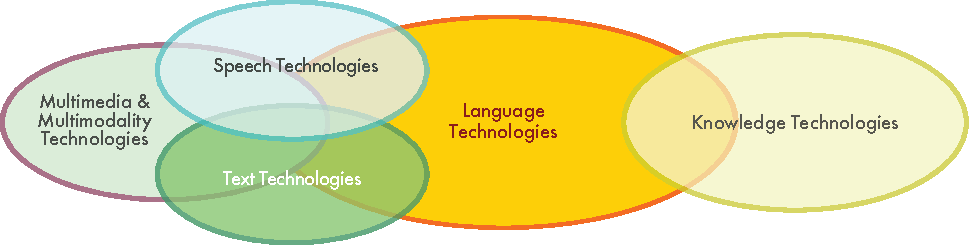
\includegraphics[width=\textwidth]{../_media/english/language_technologies}
  \caption{Language technologies}
  \label{fig:ltincontext_en}
  \colorrule{grey3}{\textwidth}{1.5pt}
\end{figure*}

Language technology is an established area of research with an extensive set of introductory literature. The interested reader is referred to the following references:  \cite{jurafsky-martin01, manning-schuetze1, lt-world1, lt-survey1}.

Before discussing the above application areas, we will briefly describe the architecture of a typical LT system.

\subsection{Application Architectures}

Typical software applications for language processing consist of several components that mirror different aspects of language and of the task they implement. Figure~\ref{fig:textprocessingarch_en} displays a highly simplified architecture that can be found in a text processing system. The first three modules deal with the structure and meaning of the text input:
\begin{itemize}
\item Pre-processing: cleaning up the data, removing formatting, detecting the input language, replacing “5è” by “cinquè” for Catalan, etc.
\item Grammatical analysis: finding the verb and its objects, modifiers and other sentence elements etc.; detecting the sentence structure.
\item Semantic analysis: disambiguation (Which meaning of apple is the right one in a given context?), resolving anaphora and referring expressions like she, the car, etc.; representing the meaning of the sentence in a machine-readable way.
\end{itemize}

\begin{figure*}[b]
  \colorrule{grey3}{\textwidth}{1.5pt}
  \center
  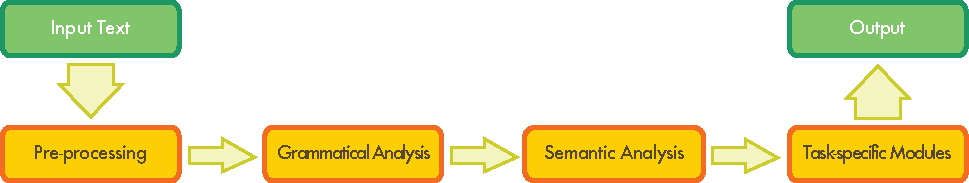
\includegraphics[width=\textwidth]{../_media/english/text_processing_app_architecture}
  \caption{A typical text processing architecture}
  \label{fig:textprocessingarch_en}
  \colorrule{grey3}{\textwidth}{1.5pt}
\end{figure*}

Task-specific modules then perform many different operations such as automatic summarisation of an input text, database lookups and many others. Below, we will illustrate core application areas and highlight their core modules. Again, the architectures of the applications are highly simplified and idealised, to illustrate the complexity of Language Technology (LT) applications in a generally understandable way. The most important tools and resources involved are set in bold text in the text and can also be found in the table at the end of the chapter.  The sections discussing the core application areas also contain an overview of the industries active in the respective field in Catalonia. 

After introducing the core application areas, we will give a short overview of the situation in LT research and education, concluding with an overview of past and ongoing research programs. At the end of this section, we will present an expert estimation on the situation regarding core LT tools and resources on a number of dimensions such as availability, maturity, or quality. This table gives a good overview on the situation of LT for Catalan.

\subsection{Core Application Areas}

    In this section, we focus on the most important LT tools and resources, and give an overview of LT activities in Catalan. Tools and resources that are set in bold in the text can also be found in the table at the end of this chapter.

\subsubsection{Language Checking}

Anyone using a word processing tool such as Microsoft Word has come across a spell checking component that indicates spelling mistakes and proposes corrections. Forty years after the first spelling correction program by Ralph Gorin, language checkers nowadays do not simply compare the list of extracted words against a dictionary of correctly spelled words, but have become increasingly sophisticated. 

\begin{figure*}[htb]
  \colorrule{grey3}{\textwidth}{1.5pt}
  \center
  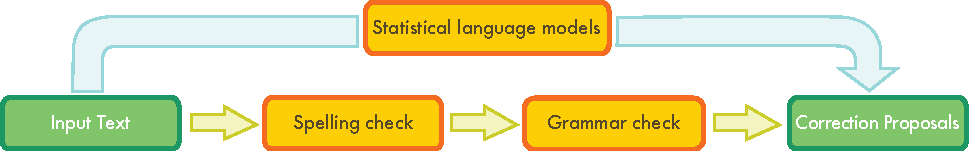
\includegraphics[width=\textwidth]{../_media/english/language_checking}
  \caption{Language checking (top: statistical; bottom: rule-based)}
  \label{fig:langcheckingaarch_en}
  \colorrule{grey3}{\textwidth}{1.5pt}
\end{figure*}

In addition to language-dependent algorithms for handling morphology (e.g. plural formation), some are now capable of recognising syntax–related errors, such as a missing verb or a verb that does not agree with its subject in person and number, e.g. in ‘She write a letter.’ 

Language checking (see figure~\ref{fig:langcheckingaarch_en}) either requires the formulation of language-specific grammar rules, i.e. a high degree of expertise and manual labour, or the use of a so-called statistical language model. Such models calculate the probability of a particular word occurring in a specific environment (i.e., the preceding and following words).

For example, ``llibre anglès'' is a much more probable word sequence than ``llibre anglesa''. A statistical language model can be automatically derived using a large amount of (correct) language data (i.e. a corpus). Up to now, these approaches have mostly been developed and evaluated on English language data. However, they do not necessarily transfer straightforwardly to Catalan with its flexible word order and richer inflection. 

The use of Language Checking is not limited to word processing tools. It is also applied in authoring support systems. Accompanying the rising number of technical products, the amount of technical documentation has rapidly increased over the last decades. Fearing customer complaints about wrong usage and damage claims resulting from bad or badly understood instructions, companies have begun to focus increasingly on the quality of technical documentation, and at the same time targeting the international market. Advances in natural language processing lead to the development of authoring support software, which assists the writer of technical documentation to use vocabulary and sentence structures consistent with certain rules and (corporate) terminology restrictions.

\boxtext{Language checking is not limited to word processors but also applies to authoring systems.}

Only a few companies and Language Service Providers offer products in this area for Catalan. Enciclopèdia Catalana, Maxigrammar and Inèdit have created and commercialised products that include spell and grammar checking for Catalan, as well as specific checking facilities adapted to different domains and styles. Softcatalà and Barcelona Media have also developed language tools that are offered to the community as web applications. A new version of “\textit{El Corrector}” has recently been developed and commercialised as iPod, iPhone and iPad apps. 

Besides spell checkers and authoring support, Language Checking is also important in the field of computer-assisted language learning and is applied to automatically correct queries sent to Web Search engines, e.g. Google’s ‘Did you mean…’ suggestions. 

\subsubsection{Web Search}

\begin{figure*}[htb]
  \colorrule{grey3}{\textwidth}{1.5pt}
  \center
  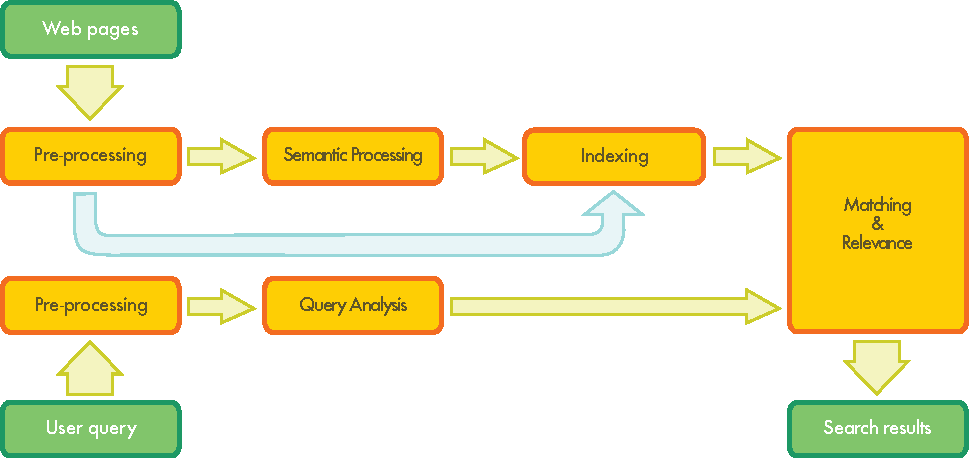
\includegraphics[width=\textwidth]{../_media/english/web_search_architecture}
  \caption{Web search architecture}
  \label{fig:websearcharch_en}
  \colorrule{grey3}{\textwidth}{1.5pt}
 \end{figure*}

Search on the web, in intranets or in digital libraries, is probably the most widely used and yet underdeveloped Language Technology today. The search engine Google, which started in 1998, is nowadays used for about 80\% of all search queries world-wide \cite{CAT-Nota22}. 

Neither the search interface nor the presentation of the retrieved results has significantly changed since the first version. In the current version, Google offers a spelling correction facility for misspelled words, including Catalan, and, in 2009, they incorporated basic semantic search capabilities into their algorithmic mix \cite{CAT-Nota23}, which can improve search accuracy by analysing the meaning of the query terms in context. The success story of Google shows that with a lot of data at hand and efficient techniques for indexing these data, a mainly statistically-based approach can lead to satisfactory results. 

However, for a more sophisticated request for information, integrating deeper linguistic knowledge is essential. In the research labs, experiments using machine-readable thesauri and ontological language resources like WordNet have shown improvements by allowing the possibility of finding a page on the basis of synonyms of the search terms, or even more loosely related terms. Again, these developments require language specific resources. A Catalan WordNet has been developed by the research centre TALP at Universitat Politècnica de Catalunya. The Catalan WordNet is freely available \cite{CAT-Nota24}.

\boxtext{The next generation of search engines\\ will have to include much more sophisticated language technology.}

The next generation of search engines will have to include much more sophisticated Language Technology. If a search query consists of a question or another type of sentence rather than a list of keywords, retrieving relevant answers to this query requires an analysis of this sentence on a syntactic and semantic level as well as the availability of an index that allows for a fast retrieval of the relevant documents. For example, imagine a user inputs the query ‘Give me a list of all companies that were taken over by other companies in the last five years’. For a satisfactory answer, \textbf{syntactic parsing} needs to be applied to analyse the grammatical structure of the sentence and determine that the user is looking for companies that have been taken over and not companies that took over others. Also, the expression last five years needs to be processed in order to find out which years it refers to. 

Finally, the processed query needs to be matched against a huge amount of unstructured data in order to find the piece or pieces of information the user is looking for. This is commonly referred to as information retrieval and involves the search for and ranking of relevant documents. In addition, generating a list of companies, we also need to extract the information that a particular string of words in a document refers to a company name. This kind of information is made available by so-called named-entity recognizers. 

Even more demanding is the attempt to match a query to documents written in a different language. For cross-lingual information retrieval, we have to automatically translate the query to all possible source languages and transfer the retrieved information back to the target language. The increasing percentage of data available in non-textual formats drives the demand for services enabling multimedia information retrieval, i.e., information search on images, audio, and video data. For audio and video files, this involves a \textbf{speech recognition} module to convert speech content into text or a phonetic representation, to which user queries can be matched.

Small and Medium Enterprises such as Inbenta \cite{CAT-inbenta} or RightNow (formerly q-go \cite{CAT-rightnow}) offer specific semantic search engines, including those that are developed for Catalan.

There are also some interesting initiatives to group specific web search services for Catalan, such as CerCat or Som-hi \cite{CAT-cercadors}, as one of the firs initiatives. An historical overview can be found at \cite{CAT-Resum-sobre-cercadors}.

\subsubsection{Speech Interaction}

\begin{figure*}[htb]
  \colorrule{grey3}{\textwidth}{1.5pt}
  \center
  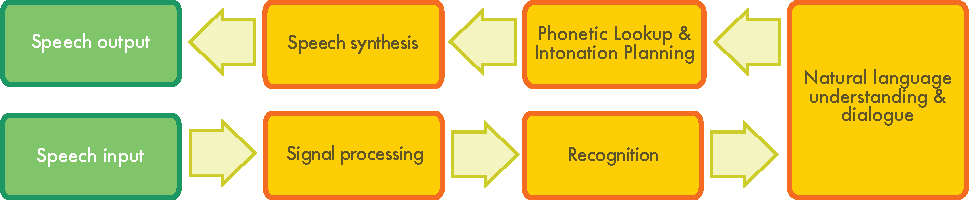
\includegraphics[width=\textwidth]{../_media/english/simple_speech-based_dialogue_architecture}
  \caption{Speech-based dialogue system}
  \label{fig:dialoguearch_en}
  \colorrule{grey3}{\textwidth}{1.5pt}
\end{figure*}

Speech interaction technology is the basis for the creation of interfaces that allow a user to interact with machines using spoken language rather than, e.g., a graphical display, a keyboard and a mouse. Today, such voice user interfaces (VUIs) are usually employed for partially or fully automating service offerings provided by companies to their customers, employees or partners via the telephone. Business domains that rely heavily on VUIs are banking, logistics, public transportation and telecommunications. Other usages of speech interaction technology are interfaces to particular devices, e.g. in-car navigation systems, and the employment of spoken language as an alternative to the input/output modalities of graphical user interfaces, e.g. in smart phones.

At its core, speech interaction comprises the following four different technologies:
\begin{itemize}
\item Automatic \textbf{speech recognition} (ASR) is responsible for determining which words were actually spoken given a sequence of sounds uttered by a user.
\item \textbf{Syntactic analysis} and \underline{semantic interpretation} deal with analysing the syntactic structure of a user’s utterance and interpret-ting the latter according to the given system’s purpose.
\item \textbf{Dialogue Management} is required for determining, on the part of the system the user interacts with, which action shall be taken given the user’s input and the system’s functionality.
\item \textbf{Speech Synthesis} (Text-to-Speech, TTS) technology is employed for transforming the wording of that utterance into sounds that will be output to the user. 
\end{itemize}
One of the major challenges is to have an ASR system recognise the words uttered by a user as precisely as possible. This requires either a restriction of the range of possible user utterances to a limi-ted set of keywords, or the manual creation of language models that cover a large range of natural language user utterances. Whereas the former results in a rather rigid and inflexible usage of a VUI and possibly causes a poor user acceptance, the creation, tuning and maintenance of language models may increase the costs significantly. However, VUIs that employ language models and initially allow a user to flexibly express their intent – evoked, e.g., by a \textit{How may I help you} greeting – show both a higher automation rate and a higher user acceptance and may therefore be considered as advantageous over a less flexible \textit{directed dialogue} approach.

\boxtext{Speech interaction is the basis for interfaces that allow a user to interact with spoken language.}

For the output part of a VUI, companies tend to use utterances pre-recorded by professional – ideally corporate – speakers a lot. For static utterances, in which the wording does not depend on the particular contexts of use or the personal data of the given user, this will result in a rich user experience. However, the more dynamic content an utterance needs to consider, the more the user experience may suffer from a poor prosody resulting from concatenating single audio files. In contrast, today’s TTS systems prove superior, though optimisable, regarding the prosodic naturalness of dynamic utterances.  

Regarding the market for speech interaction technology, the last decade has been characterised by a strong standardisation of the interfaces between the different technology components, as well as by standards for creating particular software artefacts for a given application. There also has been strong market consolidation within the last ten years, particularly in the field of ASR and TTS. Here, the national markets in the G20 countries – i.e. economically strong countries with a considerable population - are dominated by less than 5 players worldwide, with Nuance being the most prominent one in Europe, also for Catalan, although some smaller local companies are starting to compete, such as Verbio \cite{CAT-Nota25}, which is a spin-off of Universitat Politècnica de Catalunya and has its own speech technology. 

Regarding dialogue management technology and know-how, markets are strongly dominated by national players, which are usually SMEs. Most of the companies on the Catalan TTS market are essentially application developers. Key players in the Spanish market are: Indsys \cite{CAT-Nota26} (Intelligent Dialogue Systems), Fonetic \cite{CAT-Nota27}, Ydilo \cite{CAT-Nota28} and NaturalVoz \cite{CAT-Nota29}.

Looking beyond today’s state of technology, there will be significant changes due to the spread of smart phones as a new platform for managing customer relationships – in addition to the telephone, internet, and email channels. This tendency will also affect the employment of technology for speech interaction. On one hand, demand for telephony-based VUIs will decrease, in the long run. On the other hand, the usage of spoken language as a user-friendly input modality for smart phones will gain significant importance. This tendency is supported by the observable improvement of speaker independent speech recognition accuracy for speech dictation services that are already offered as centralised services to smart phone users. Given this ‘outsourcing’ of the recognition task to the infrastructure of applications, the application-specific employment of linguistic core technologies will supposedly gain importance compared to the present situation. 

\subsubsection{Machine Translation}

The idea of using digital computers for translation of natural languages came up in 1946 by A. D. Booth and was followed by substantial funding for research in this area in the 1950s and beginning again in the 1980s. Nevertheless, \textbf{Machine Translation} (MT) still fails to fulfil the high expectations it gave rise to in its early years. 

\boxtext{At its basic level, Machine Translation simply substitutes words in one natural language with words in another language.}

\begin{figure*}[htb]
  \colorrule{grey3}{\textwidth}{1.5pt}
  \center
  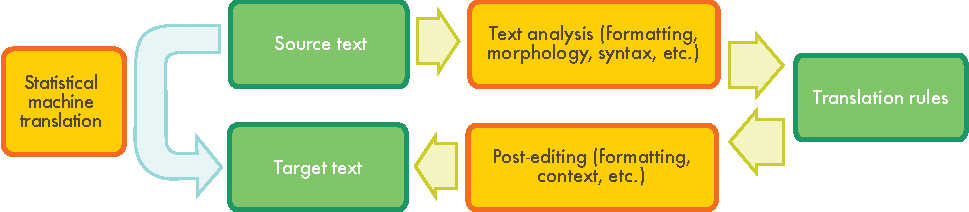
\includegraphics[width=\textwidth]{../_media/english/machine_translation}
  \caption{Machine translation (left: statistical; right: rule-based)}
  \label{fig:mtarch_en}
  \colorrule{grey3}{\textwidth}{1.5pt}
\end{figure*}

At its basic level, MT simply substitutes words in one natural language by words in another. This can be useful in subject domains with a very restricted, formulaic language, e.g., weather reports or for closely related languages. However, for a good translation of less standardised texts, larger text units (phrases, sentences, or even whole passages) need to be matched to their closest counterparts in the target language. The major difficulty here lies in the fact that human language is ambiguous, which yields challenges on multiple levels, e.g., word sense disambiguation at the lexical level (‘Jaguar’ can mean a car or an animal) or the attachment of prepositional phrases on the syntactic level as in:
\begin{itemize}
\item \textit{Passejava amb el nen cantant.}
\item \textit{T1: I was walking with the singer child.}
\item \textit{T2: I was walking and singing with the child.}
\end{itemize}

One way of approaching the task is based on linguistic rules. For translations between closely related languages, a direct translation may be feasible in cases like the example above. But often rule-based (or knowledge-driven) systems analyse the input text and create an intermediary, symbolic representation, from which the text in the target language is generated. The success of these methods is highly dependent on the availability of extensive \textbf{lexica} with morphological, syntactic, and semantic information, and large sets of \textbf{grammar rules} carefully designed by a skilled linguist.

Beginning in the late 1980s, as computational power increased and became less expensive, more interest was shown in statistical mo-dels for MT. The parameters of these statistical models are derived from the analysis of bilingual text corpora, such as the Europarl parallel corpus, which contains the proceedings of the European Parliament in 21 European languages. Given enough data, statistical MT works well enough to derive an approximate meaning of a foreign language text. However, unlike knowledge-driven systems, statistical (or data-driven) MT often generates ungrammatical output. On the other hand, besides the advantage that less human effort is required for grammar writing, data-driven MT can also cover particularities of the language that go missing in knowledge-driven systems, for example idiomatic expressions. 

As the strengths and weaknesses of knowledge- and data-driven MT are complementary, researchers nowadays unanimously target hybrid approaches combining methodologies of both. This can be done in several ways. One is to use both knowledge- and data-driven systems and have a selection module decide on the best output for each sentence. However, for longer sentences, no result will be perfect. A better solution is to combine the best parts of each sentence from multiple outputs, which can be fairly complex, as corresponding parts of multiple alternatives are not always obvious and need to be aligned. 

Due to the particular official situation of bilingualism in particular regions of Spain, and to the linguistic relatedness of Catalan with Spanish, the development of MT systems for this pair of languages has been quite successful. Initially supported by the autonomous Catalan leading MT systems like METAL (Siemens), ATLAS (Fujitsu) were located in Barcelona during the 1990’s, and when the big companies ended their engagement, the systems were further developed by offspring and spin-off companies: METAL was further developed by a local SME, INCYTA, as well as by GMS and later by Lucy Software, which is currently the main (but not the only) vendor for MT systems involving Catalan. In fact, the Catalan-Spanish MT system  bought by the Generalitat of Catalonia was offered as a public web service as early as 2005, while Google started offering it in 2007. 

Other companies also developed MT systems with in-house technologies: T6 Estàndar Linguistic and AutomaticTrans. The system developed by AutomaticTrans has its origin in the production of a bilingual newspaper, in Catalan and Spanish, El Periódico. Currently, there are three newspapers which are made available in the two languages  through the use of Machine Translation technology. The other two are El Segre and La Vanguardia. 

The Generalitat Valenciana supported the creation of a MT system specific for Valencian, SALT. More recently, the Universidad Politécnica de Valencia has also released a version of SiShiTra, a hybrid system, and the open-source OpenTrad also offers a particular version for Valencian.

The pair Spanish-Catalan was the origin of the open source system developed by the Transducens \cite{CAT-transducens} group of the Universitat d'Alacant \cite{CAT-UnivAlacant}, Apertium, which is the first open-source MT technology in the world. Its commercial exploitation is mainly carried out by Prompsit Language Engineering and OpenTrad Consortium. 

Most of the systems introduced above are rule-based. While there is significant research on this technology in national and international contexts, data-driven and hybrid systems have been less successful in business than in research so far. 

Provided with good adaptation in terms of user-specific terminology and workflow integration, the use of MT can increase productivity significantly. Thus, the main user of MT for Catalan is the public administration, including the Justice Department and other Ministries, since the beginning of the 21st century. 

The quality of MT systems is still considered to have huge improvement potential. Challenges include the adaptability of the language resources to a given subject domain or user area and the integration into existing workflows with term bases and translation memories.

In addition, most of the existing parallel corpora are between Spanish and Catalan, so for the majority of translation solutions, Spanish is the pivot language.

Evaluation campaigns help to compare the quality of MT systems, their approaches and the status of the systems for different language pairs. Figure~\ref{fig:euromatrix_en} (p.~\pageref{fig:euromatrix_en}), which was prepared during the Euromatrix+ project, shows the pair-wise performances obtained for 22 of the 23 EU languages (Irish was not compared). The results are ranked according to a BLEU score, which indicates higher scores for better translations \cite{bleu1}. A human translator would normally achieve around 80 points. The best results (in green and blue) were achieved by languages that benefit from a considerable research effort in coordinated programmes and the existence of many parallel corpora (e.\,g., English, French, Dutch, Spanish and German). The languages with poorer results are shown in red. These either lack such development efforts or are structurally very different from other languages (e.\,g., Hungarian, Maltese, Finnish).

\subsection{Other Application Areas}

Building Language Technology applications involves a range of subtasks that do not always surface at the level of interaction with the user, but provide significant service functionalities ‘under the hood’ of the system. Therefore, they constitute important research issues that have become individual sub-disciplines of Computational Linguistics in academia. 

Question answering has become an active area of research, for which annotated corpora have been built and scientific competitions have been started.

The idea is to move from keyword-based search (to which the engine responds with a whole collection of potentially relevant documents) to the scenario of the user asking a concrete question and the system providing a single answer: \\
\begin{itemize}
\item[] \textit{Question: At what age did Neil Armstrong step on the moon?}
\item[] \textit{Answer: 38.}
\end{itemize}

While this is obviously related to the aforementioned core area Web Search, question answering nowadays is primarily an umbrella term for research questions such as what types of questions should be distinguished and how should they be handled, how can a set of documents that potentially contain the answer be analysed and compared (do they give conflicting answers?), and how can specific information - the answer - be reliably extracted from a document, without unduly ignoring the context. 

\boxtext{Language technology applications often provide significant service functionalities behind the scenes of larger software systems.}

This is in turn related to the information extraction (IE) task, an area that was extremely popular and influential at the time of the ‘statistical turn’ in Computational Linguistics, in the early 1990s. IE aims at identifying specific pieces of information in specific classes of documents; this could e.g. be the detection of the key players in company takeovers as reported in newspaper stories. Another scenario that has been worked on is reports on terrorist incidents, where the problem is to map the text to a template specifying the perpetrator, the target, time and location of the incident, and the results of the incident. Domain-specific template-filling is the central characteristic of IE, which for this reason is another example of a ‘behind the scenes’ technology that constitutes a well-demarcated research area but for practical purposes then needs to be embedded into a suitable application environment. 

Two ‘borderline’ areas, which sometimes play the role of standalone application and sometimes that of supportive, ‘under the hood’ component are text summarization and text generation. Summarization, obviously, refers to the task of making a long text short, and is offered for instance as a functionality within MS Word. It works largely on a statistical basis, by first identifying ‘important’ words in a text (that is, for example, words that are highly frequent in this text but markedly less frequent in general language use) and then determining those sentences that contain many important words. These sentences are then marked in the document, or extracted from it, and are taken to constitute the summary. In this scenario, which is by far the most popular one, summarization equals sentence extraction: the text is reduced to a subset of its sentences. All commercial summarizers make use of this idea. An alternative approach, to which some research is devoted, is to actually synthesize new sentences, i.e., to build a summary of sentences that need not show up in that form in the source text. This requires a certain amount of deeper understanding of the text and therefore is much less robust. All in all, a text generator is in most cases not a stand-alone application but embedded into a larger software environment, such as into the clinical information system where patient data is collected, stored and processed, and report generation is just one of many functionalities.

\boxtext{For Catalan and for most languages, research in most text technologies is much less developed than for English.}

The situation in all these research areas for most of the languages is much less developed than it is for English, where question answering, information extraction, and summarization have since the 1990s been the subject of numerous open competitions, primarily those organised by DARPA/NIST in the United States. These have significantly improved the state of the art, but the focus has always been on English; some competitions have added multilingual tracks, but Catalan has never been prominent. Accordingly, there are hardly any annotated corpora or other resources for Catalan that relate to these tasks. Summarization systems, when using purely statistical methods, are often to a good extent language-independent, and thus some research prototypes are available. For text generation, reusable components have traditionally been limited to the surface realisation modules (the "generation grammars"); again, most available software is for English.

\subsection{Educational Programmes}

Language Technology is a highly interdisciplinary field, involving the expertise of linguists, computer scientists, mathematicians, philosophers, psycholinguists, and neuroscientists, among others. Although it has not yet acquired a fixed place in any of the faculty systems of the universities in the Catalan linguistic domain, Barcelona has a higher concentration of studies that consider the field. 
Several subjects related to language technology are offered in bachelor degrees by different departments, such as the faculty of computer science (e.g., in the Universitat d’Alacant) or the faculty of linguistics (e.g., in the Universitat de Barcelona, the Universitat PompeuFabra and the Universitat Oberta de Catalunya).
As regards masters courses and postgraduate degrees, Universitat Autònoma de Barcelona offers the International Master in Natural Language Processing and Human Language Technology, in collaboration with foreign universities. Besides this, some masters are offered in which one of the research areas focusses on natural language processing (e.g., the Universitat de Barcelona, the Universitat Pompeu Fabra, the Universitat de Girona and the Universitat Rovira i Virgili). Modules in Language Technology are also offered to students of other master courses (e.g. the Universitat d’Alacant, the Universitat de Castelló and the Universitat Politècnica de València). 
PhD programmes are also offered, in which one of the research areas is human language technologies (e.g. the Universitat d’Alacant, the Universitat de Barcelona and the Universitat Rovira i Virgili).

\subsection{National Projects and Efforts}

Technology programs for the Catalan language have been supported by the Spanish and the Catalan Governments.

The existence of comparably lively LT activity, specifically in the Barcelona area, can be traced back to major LT programs and large research projects carried out in the last decades. One of the first programs was EUROTRA, the ambitious Machine Translation (MT) project established and funded by the European Commission from the late 1970s until 1994. Even though the EUROTRA project did not work with Catalan, the project, which had a long-term impact on language industries in Europe, was also crucial to highlighting the importance of languages in the technological world, and how it could affect small to medium languages. The Catalan government quickly began to understand the challenges and initiated different programs that basically addressed the localization of differrent software tools, including LT applications. 

Machine translation, speech recognition, spelling and grammar checking research and industrial developments have been supported by different departments of the Generalitat de Catalunya for more than 20 years. The Secretaria de Política Lingüística, the Comissionat per a la Societat de la Informació and the Secretaria de Telecomunicacions i Societat de la Informació have been the main engines of the support policies. Besides, MT into or from Catalan has also benefited from Spanish funding programs. Projects such as Apertium (open source MT system) and OpenTrad, as well as a number of other small programs, have received funding from the Ministerio de Ciencia y Tecnología. 

The CREL – Centre de Referència en Enginyeria Lingüística, 1996-2000, managed by the Institut d’Estudis Catalans and with participants from the major Catalan Universities, was created with the specific aim of promoting the creation of resources and tools for the automatic processing of Catalan texts in a variety of applications. 

As regards the presence of the Catalan language in European infrastructures, in 2008 the Catalan Government signed an agreement with Universitat Pompeu Fabra, the national representative of the European project CLARIN in Spain, with the aim of building a Catalan demonstrator. The main goal of this demonstrator (CLARIN-CAT-LAB), which is already available for research purposes \cite{CAT-Nota30}, is to integrate language resources and technology for the Catalan language, thus guaranteeing the presence of this language in the European CLARIN infrastructure. In addition, the Biblioteca de Catalunya, Catalonia’s national library, is one of the partners in the EUROPEANA project. Other Catalan institutions are also contributing content to the project.

From 2000 up until the present day, the Spanish Government supported several projects in the area of multilingual speech technologies within the National Plan of Research and Technology, i.e., TEHAM, AVIVAVOZ, and BUCEADOR. The main purpose of these projects was to improve the quality of speech recognition, speech translation and text to speech synthesis in all the official languages spoken in Spain, i.e., Basque, Galician, Catalan and Spanish.

In 2005, the Catalan Government launched a project to produce Language Resources for Speech Recognition and Speech Synthesis. As a result, Language Resources for telephone applications, in-car applications and microphone applications were produced. Later, the project TECNOPARLA (2007-2010) had as its objective the translation of speech between Spanish and Catalan. The speech signals were collected directly from TV programmes. The project resulted on advances in all the component speech technologies, i.e.  diarization, speech recognition, speech translation and text to speech synthesis.
  
\subsection{Availability of Tools and Resources}

    The following table summarises the current state of language technology support for the German language. The rating for existing tools and resources was generated by leading experts in the field who provided estimates based on a scale from 0 (very low) to 6 (very high) according to seven criteria.

\begin{figure*}[htb]
\centering
%\begin{tabular}{>{\columncolor{orange1}}p{.33\linewidth}ccccccc} % ORIGINAL
\begin{tabular}{>{\columncolor{orange1}}p{.33\linewidth}@{\hspace*{6mm}}c@{\hspace*{6mm}}c@{\hspace*{6mm}}c@{\hspace*{6mm}}c@{\hspace*{6mm}}c@{\hspace*{6mm}}c@{\hspace*{6mm}}c}
\rowcolor{orange1}
 \cellcolor{white}&\begin{sideways}\makecell[l]{Quantity}\end{sideways}
&\begin{sideways}\makecell[l]{\makecell[l]{Availability} }\end{sideways} &\begin{sideways}\makecell[l]{Quality}\end{sideways}
&\begin{sideways}\makecell[l]{Coverage}\end{sideways} &\begin{sideways}\makecell[l]{Maturity}\end{sideways} &\begin{sideways}\makecell[l]{Sustainability}\end{sideways} &\begin{sideways}\makecell[l]{Adaptability}\end{sideways} \\ \addlinespace
\multicolumn{8}{>{\columncolor{orange2}}l}{Language Technology: Tools, Technologies and Applications} \\ \addlinespace
Speech Recognition	&3&3&3&3&3&3&2 \\ \addlinespace
Speech Synthesis &4&2&4&4&5&4&2\\ \addlinespace
Grammatical analysis &3&2.5&4&4&4&2.5&2.5\\ \addlinespace
Semantic analysis &1&1&2&1&1&1&1\\ \addlinespace
Text generation &1&2&3&1&3&3&1\\ \addlinespace
Machine translation &3&3&2&3&4&1&2\\ \addlinespace
\multicolumn{8}{>{\columncolor{orange2}}l}{Language Resources: Resources, Data and Knowledge Bases} \\ \addlinespace
Text corpora &3&2.5&3.5&3&3&2.5&2.5\\ \addlinespace
Speech corpora &3&5&3&2&3&3&2\\ \addlinespace
Parallel corpora &2&1&2&2&2&1&1\\ \addlinespace
Lexical resources &2.5&2&3&2.5&3&3&2.5\\ \addlinespace
Grammars &2&3&2&2&2&2&2\\
\end{tabular}
\caption{State of language technology support for Catalan}
\label{fig:lrlttable_en}
\end{figure*}

The table can be summarized in the form of a number of key messages, which highlight crucial issues for the further development of automatic language processing of Catalan, on the basis of the present situation:

\begin{itemize}
\item While some specific corpora of high quality exist, a very large syntactically annotated corpus is not available.
\item For Catalan, a large corpus exists, but it is not easily/cheaply accessible.
\item Many of the resources lack standardisation, i.e., even if they exist, sustainability is not given; concerted programs and initiatives are needed to standardise data and interchange formats.
\item Semantics is more difficult to process than syntax; text semantics is more difficult to process than word and sentence semantics.
\item The more semantics a tool takes into account, the more difficult it is to find the right data; more efforts for supporting deep processing are needed.
\item Standards do exist for semantics in the sense of world knowledge (RDF, OWL, etc.); they are, however, not easily applicable to NLP tasks.
\item Speech processing is currently more mature than NLP for written text.
\item There are many groups working in machine translation, particularly focused in Catalan-Spanish. 
\item Research has been successful in designing particular high quality software, but it is nearly impossible to come up with sustainable and standardised solutions, given the current funding situations.
\end{itemize}

\subsection{Cross-language comparison}

    The current state of LT support varies considerably from one language community to another. In order to compare the situation between languages, this section will present an evaluation based on two sample application areas (machine translation and speech processing) and one underlying technology (text analysis), as well as basic language resources needed for building LT applications. 

\begin{figure*}[tb]
  \small
  \centering
  \begin{tabular}
  { % defines color for each column.
  >{\columncolor{corange5}}p{.13\linewidth}@{\hspace{.040\linewidth}}
  >{\columncolor{corange4}}p{.13\linewidth}@{\hspace{.040\linewidth}}
  >{\columncolor{corange3}}p{.13\linewidth}@{\hspace{.040\linewidth}}
  >{\columncolor{corange2}}p{.13\linewidth}@{\hspace{.040\linewidth}}
  >{\columncolor{corange1}}p{.13\linewidth} 
  }
\rowcolor{orange1} % redefines color for all columns in row 1
\begin{center}\vspace*{-2mm}\textbf{Excellent}\end{center} & 
\begin{center}\vspace*{-2mm}\textbf{Good}\end{center} & 
\begin{center}\vspace*{-2mm}\textbf{Moderate}\end{center} & 
\begin{center}\vspace*{-2mm}\textbf{Fragmentary}\end{center} & 
\begin{center}\vspace*{-2mm}\textbf{Weak/no}\end{center} \\ \addlinespace
  
& \vspace*{0.5mm}English
& \vspace*{0.5mm}
Czech \newline 
Dutch \newline 
Finnish \newline 
French \newline 
German \newline   
Italian \newline  
Portuguese \newline 
Spanish \newline
& \vspace*{0.5mm}Basque \newline 
Bulgarian \newline 
\textbf{Catalan} \newline 
Danish \newline 
Estonian \newline 
Galician\newline 
Greek \newline  
Hungarian  \newline
Irish \newline  
Norwegian \newline 
Polish \newline 
Serbian \newline 
Slovak \newline 
Slovene \newline 
Swedish \newline
& \vspace*{0.5mm}
Croatian \newline 
Icelandic \newline  
Latvian \newline 
Lithuanian \newline 
Maltese \newline 
Romanian\\
\end{tabular}
\caption{Speech processing: state of language technology support for 30 European languages}
\label{fig:speech_cluster_en}
\end{figure*}

\begin{figure*}[tb]
  \small
  \centering
  \begin{tabular}
  { % defines color for each column.
  >{\columncolor{corange5}}p{.13\linewidth}@{\hspace{.040\linewidth}}
  >{\columncolor{corange4}}p{.13\linewidth}@{\hspace{.040\linewidth}}
  >{\columncolor{corange3}}p{.13\linewidth}@{\hspace{.040\linewidth}}
  >{\columncolor{corange2}}p{.13\linewidth}@{\hspace{.040\linewidth}}
  >{\columncolor{corange1}}p{.13\linewidth} 
  }
\rowcolor{orange1} % redefines color for all columns in row 1
\begin{center}\vspace*{-2mm}\textbf{Excellent}\end{center} & 
\begin{center}\vspace*{-2mm}\textbf{Good}\end{center} & 
\begin{center}\vspace*{-2mm}\textbf{Moderate}\end{center} & 
\begin{center}\vspace*{-2mm}\textbf{Fragmentary}\end{center} & 
\begin{center}\vspace*{-2mm}\textbf{Weak/no}\end{center} \\ \addlinespace
  
& \vspace*{0.5mm} English 
& \vspace*{0.5mm} 
French \newline 
Spanish
& \vspace*{0.5mm}
\textbf{Catalan} \newline 
Dutch \newline 
German \newline 
Hungarian \newline
Italian \newline 
Polish \newline 
Romanian \newline 
& \vspace*{0.5mm}Basque \newline 
Bulgarian \newline 
Croatian \newline 
Czech \newline
Danish \newline 
Estonian \newline 
Finnish \newline 
Galician \newline 
Greek \newline 
Icelandic \newline 
Irish \newline 
Latvian \newline 
Lithuanian \newline 
Maltese \newline 
Norwegian \newline 
Portuguese \newline 
Serbian \newline 
Slovak \newline 
Slovene \newline 
Swedish \newline 
\end{tabular}
\caption{Machine translation: state of language technology support for 30 European languages}
\label{fig:mt_cluster_en}
\end{figure*}

\begin{figure*}[tb]
  \small
  \centering
  \begin{tabular}
  { % defines color for each column.
  >{\columncolor{corange5}}p{.13\linewidth}@{\hspace{.040\linewidth}}
  >{\columncolor{corange4}}p{.13\linewidth}@{\hspace{.040\linewidth}}
  >{\columncolor{corange3}}p{.13\linewidth}@{\hspace{.040\linewidth}}
  >{\columncolor{corange2}}p{.13\linewidth}@{\hspace{.040\linewidth}}
  >{\columncolor{corange1}}p{.13\linewidth} 
  }
\rowcolor{orange1} % redefines color for all columns in row 1
\begin{center}\vspace*{-2mm}\textbf{Excellent}\end{center} & 
\begin{center}\vspace*{-2mm}\textbf{Good}\end{center} & 
\begin{center}\vspace*{-2mm}\textbf{Moderate}\end{center} & 
\begin{center}\vspace*{-2mm}\textbf{Fragmentary}\end{center} & 
\begin{center}\vspace*{-2mm}\textbf{Weak/no}\end{center} \\ \addlinespace

& \vspace*{0.5mm}English
& \vspace*{0.5mm}
  Dutch \newline 
  French \newline 
  German \newline 
  Italian \newline 
  Spanish
& \vspace*{0.5mm}Basque \newline 
  Bulgarian \newline 
  \textbf{Catalan} \newline 
  Czech \newline 
  Danish \newline 
  Finnish \newline 
  Galician \newline 
  Greek \newline 
  Hungarian \newline 
  Norwegian \newline 
  Polish \newline 
  Portuguese \newline 
  Romanian \newline 
  Slovak \newline 
  Slovene \newline 
  Swedish \newline 
& \vspace*{0.5mm}
  Croatian \newline 
  Estonian \newline 
  Icelandic \newline 
  Irish \newline 
  Latvian \newline 
  Lithuanian \newline 
  Maltese \newline 
  Serbian \\
  \end{tabular}
\caption{Text analysis: state of language technology support for 30 European languages}
\label{fig:text_cluster_en}
\end{figure*}

\begin{figure*}[tb]
  \small
  \centering
  \begin{tabular}
  { % defines color for each column.
  >{\columncolor{corange5}}p{.13\linewidth}@{\hspace{.040\linewidth}}
  >{\columncolor{corange4}}p{.13\linewidth}@{\hspace{.040\linewidth}}
  >{\columncolor{corange3}}p{.13\linewidth}@{\hspace{.040\linewidth}}
  >{\columncolor{corange2}}p{.13\linewidth}@{\hspace{.040\linewidth}}
  >{\columncolor{corange1}}p{.13\linewidth} 
  }
\rowcolor{orange1} % redefines color for all columns in row 1
\begin{center}\vspace*{-2mm}\textbf{Excellent}\end{center} & 
\begin{center}\vspace*{-2mm}\textbf{Good}\end{center} & 
\begin{center}\vspace*{-2mm}\textbf{Moderate}\end{center} & 
\begin{center}\vspace*{-2mm}\textbf{Fragmentary}\end{center} & 
\begin{center}\vspace*{-2mm}\textbf{Weak/no}\end{center} \\ \addlinespace
    
& \vspace*{0.5mm}English
& \vspace*{0.5mm} 
    Czech \newline 
    Dutch \newline 
    French \newline 
    German \newline 
    Hungarian \newline
    Italian \newline
    Polish \newline
    Spanish \newline
    Swedish \newline 
& \vspace*{0.5mm} Basque\newline 
    Bulgarian\newline 
    \textbf{Catalan} \newline 
    Croatian \newline 
    Danish \newline 
    Estonian \newline 
    Finnish \newline 
    Galician \newline 
    Greek \newline 
    Norwegian \newline 
    Portuguese \newline 
    Romanian \newline 
    Serbian \newline 
    Slovak \newline 
    Slovene \newline
&  \vspace*{0.5mm}
    Icelandic \newline 
    Irish \newline 
    Latvian \newline 
    Lithuanian \newline 
    Maltese  \\
  \end{tabular}
  \caption{Speech and text resources: State of support for 30 European languages}  
  \label{fig:resources_cluster_en}
\end{figure*}

The current state of LT support varies considerably from one language community to another. In order to compare the situation between languages, this section will present an evaluation based on two sample application areas (machine translation and speech processing) and one underlying technology (text analysis), as well as basic resources needed for building LT applications. The languages were categorised using the following five-point scale: 

\begin{enumerate}
\item Excellent support
\item Good support
\item Moderate support
\item Fragmentary support
\item Weak or no support
\end{enumerate}

LT support was measured according to the following criteria:

\textbf{Speech Processing:} Quality of existing speech recognition technologies, quality of existing speech synthesis technologies, coverage of domains, number and size of existing speech corpora, amount and variety of available speech-based applications.

\textbf{Machine Translation:} Quality of existing MT technologies, number of language pairs covered, coverage of linguistic phenomena and domains, quality and size of existing parallel corpora, amount and variety of available MT applications.

\textbf{Text Analysis:} Quality and coverage of existing text analysis technologies (morphology, syntax, semantics), coverage of linguistic phenomena and domains, amount and variety of available applications, quality and size of existing (annotated) text corpora, quality and coverage of existing lexical resources (e.\,g., WordNet) and grammars.

\textbf{Resources:} Quality and size of existing text corpora, speech corpora and parallel corpora, quality and coverage of existing lexical resources and grammars.

The above tables show that, thanks to LT funding programs from the Spanish and Catalonian governments in recent decades, the Catalan language is equipped as most of other European languages. It compares well with languages with a similar number of speakers such as Hungarian, Greek, and European Portuguese despite these are official languages of EU countries. But LT resources and tools for Catalan clearly do not yet reach the quality and coverage of comparable resources and tools for the Spanish language, which is in a good position in almost all LT areas. And there are still plenty of gaps in Spanish language resources with regard to high quality applications.

For speech processing, current technologies perform well enough to be successfully integrated into a number of industrial applications such as Interactive Voice Response systems and constrained domain dictation systems. Machine Translation systems get a good performance, especially between the language pairs Spanish-Catalan and English-Catalan. However, for building more sophisticated applications, such as machine translation, there is a clear need for resources and technologies that cover a wider range of linguistic aspects and allow a deep semantic analysis of the input text. By improving the quality and coverage of these basic resources and technologies, we shall be able to open up new opportunities for tackling a vast range of advanced application areas, including high-quality machine translation.  

\subsection{Conclusions}

    \emph{In this series of white papers, we have made an important initial effort to assess language technology support for 30 European languages, and provide a high-level comparison across these languages. By identifying the gaps, needs and deficits, the European language technology community and related stakeholders are now in a position to design a large scale research and development programme aimed at building a truly multilingual, technology-enabled Europe.}

The results of this white paper series show that there is a dramatic difference in language technology support between the various European languages. While there are good quality software and resources available for some languages and application areas, others (usually ‘smaller’ languages) have substantial gaps. Many languages lack basic technologies for text analysis and the essential resources for developing these technologies. Others have basic tools and resources but are as yet unable to invest in semantic processing. We therefore still need to make a large-scale effort to attain the ambitious goal of providing high-quality machine translation between all European languages. 

    In the case of the Catalan language, we are moderately optimistic about the current state of language technology support. There is a viable LT research community in Catalonia, which has been supported by Spanish and Catalan research programmes. A number of resources and state-of-the-art technologies have been produced and distributed for Catalan. However, the scope of the resources and the range of tools are still very limited when compared to the resources and tools for the Spanish language (and obviously for the English language) and they are simply not sufficient in quality and quantity to develop the kind of technologies required to support a truly multilingual knowledge society.

    The Catalan language technology industry dedicated to transforming research into products is currently very small. Most large companies have either stopped or severely cut their LT efforts, leaving the languages spoken by a small number of people in a secondary objective.

    Our findings show that the only alternative is to make a substantial effort to create LT resources for Catalan, and use them to drive forward research, innovation and development. The need for large amounts of data and the extreme complexity of language technology systems makes it vital to develop a new infrastructure and a more coherent research organization to spur greater sharing and cooperation.

    There is also a lack of continuity in research and development funding. Short-term coordinated programmes tend to alternate with periods of sparse or zero funding. In addition, there is an overall lack of coordination with programmes in other EU countries and at the European Commission level.

    We can therefore conclude that there is a desperate need for a large, coordinated initiative focused on overcoming the differences in language technology readiness for European languages as a whole.

    META-NET’s long-term goal is to introduce high-quality language technology for all languages in order to achieve political and economic unity through cultural diversity. The technology will help tear down existing barriers and build bridges between Europe’s languages. This requires all stakeholders - in politics, research, business, and society - to unite their efforts for the future. 
\end{multicols}

\clearpage


% --------------------------------------------------------------------------
\ssection[About META-NET]{About META-NET}

\begin{multicols}{2}
META-NET is a Network of Excellence funded by the European Commission. The network currently consists of 54 members from 33 European countries \cite{rehm2011}. META-NET fosters the Multilingual Europe Technology Alliance (META), a growing community of language technology professionals and organisations in Europe. META-NET cooperates with other initiatives like the Common Language Resources and Technology Infrastructure (CLARIN), which is helping to establish digital humanities research in Europe. META-NET fosters the technological foundations for a truly multilingual European information society that:

\begin{itemize}
\item makes communication and cooperation possible across languages;
\item provides equal access to information and knowledge in any language;
\item offers advanced and affordable networked information technology to European citizens.
\end{itemize}

META-NET stimulates and promotes multilingual technologies for all European languages. The technologies enable automatic translation, content production, information processing and knowledge management for a wide variety of applications and subject domains. The network wants to improve current approaches, so better communication and cooperation across languages can take place. Europeans have an equal right to information and knowledge regardless of language.

META-NET launched on 1 February 2010 with the goal of advancing research in language technology (LT). The network supports a Europe that unites as a single digital market and information space. META-NET has conducted several activities that further its goals. META-VISION, META-SHARE and META-RESEARCH are the network’s three lines of action.

\textbf{META-VISION} fosters a dynamic and influential stakeholder community that unites around a shared vision and a common strategic research agenda (SRA). The main focus of this activity is to build a coherent and cohesive LT community in Europe by bringing together representatives from highly fragmented and diverse groups of stakeholders. In the first year of META-NET, presentations at the FLaReNet Forum (Spain), Language Technology Days (Luxembourg), JIAMCATT 2010 (Luxembourg), LREC 2010 (Malta), EAMT 2010 (France) and ICT 2010 (Belgium) centred on public outreach. According to initial estimates, META-NET has already contacted more than 2,500 LT professionals to develop its goals and visions with them. At the META-FORUM 2010 event in Brussels, META-NET communicated the initial results of its vision building process to more than 250 participants. In a series of interactive sessions, the participants provided feedback on the visions presented by the network. 

\textbf{META-SHARE} creates an open, distributed facility for exchanging and sharing resources. The peer-to-peer network of repositories will contain language data, tools and web services that are documented with high-quality metadata and organised in standardised categories. The resources can be readily accessed and uniformly searched. The available resources include free, open source materials as well as restricted, commercially available, fee-based items. META-SHARE targets existing language data, tools and systems as well as new and emerging products that are required for building and evaluating new technologies, products and services. The reuse, combination, repurposing and re-engineering of language data and tools plays a crucial role. META-SHARE will eventually become a critical part of the LT marketplace for developers, localisation experts, researchers, translators and language professionals from small, mid-sized and large enterprises. META-SHARE addresses the full development cycle of LT—from research to innovative products and services. A key aspect of this activity is establishing META-SHARE as an important and valuable part of a European and global infrastructure for the LT community. 

\textbf{META-RESEARCH} builds bridges to related technology fields. This activity seeks to leverage advances in other fields and to capitalise on innovative research that can benefit language technology. In particular, this activity wants to bring more semantics into machine translation (MT), optimise the division of labour in hybrid MT, exploit context when computing automatic translations and prepare an empirical base for MT. META-RESEARCH is working with other fields and disciplines, such as machine learning and the Semantic Web community. META-RESEARCH focuses on collecting data, preparing data sets and organising language resources for evaluation purposes; compiling inventories of tools and methods; and organising workshops and training events for members of the community. This activity has already clearly identified aspects of MT where semantics can impact current best practices. In addition, the activity has created recommendations on how to approach the problem of integrating semantic information into MT. META-RESEARCH is also finalising a new language resource for MT, the Annotated Hybrid Sample MT Corpus, which provides data for English-German, English-Spanish and English-Czech language pairs. META-RESEARCH has also developed software that collects multilingual corpora that are hidden on the Web.
\end{multicols}

\vfill
\centerline{office@meta-net.eu -- http://www.meta-net.eu}

\cleardoublepage

\appendix
\addtocontents{toc}{\protect\bigskip}

\bsection[Referències -- References]{Referències --- References}
\bibliographystyle{unsrt} % What is the difference between "unsrt" und "is-unsrt"?
%\bibliographystyle{is-unsrt}
\bibliography{catalan_references}
  
\cleardoublepage

\bsection[Membres de META-NET -- META-NET Members]{Membres de META-NET --- META-NET Members}
\label{metanetmembers}

\small

\begin{longtable}{@{}llp{113mm}@{}}
  Alemanya & \textcolor{grey1}{Germany} & Language Technology Lab, DFKI: Hans Uszkoreit, Georg Rehm\\ \addlinespace
  & & Human Language Technology and Pattern Recognition, RWTH Aachen University: Hermann Ney \\ \addlinespace
  & & Department of Computational Linguistics, Saarland University: Manfred Pinkal\\ \addlinespace Dänemark &  \textcolor{grey1}{Denmark} & Centre for Language Technology, University of Copenhagen: \newline Bolette Sandford Pedersen, Bente Maegaard\\ \addlinespace
  Àustria & \textcolor{grey1}{Austria} & Zentrum für Translationswissenschaft, Universität Wien: Gerhard Budin\\ \addlinespace 
  Bèlgica & \textcolor{grey1}{Belgium} & Computational Linguistics and Psycholinguistics Research Centre, University of Antwerp: Walter Daelemans\\ \addlinespace
  & & Centre for Processing Speech and Images, University of Leuven: Dirk van Compernolle \\ \addlinespace
  Bulgària & \textcolor{grey1}{Bulgaria} & Institute for Bulgarian Language, Bulgarian Academy of Sciences: Svetla Koeva \\ \addlinespace
  Croàcia & \textcolor{grey1}{Croatia} & Institute of Linguistics, Faculty of Humanities and Social Science, University of Zagreb: Marko Tadić \\ \addlinespace
  Eslovàquia & \textcolor{grey1}{Slovakia} & Ľudovít Štúr Institute of Linguistics, Slovak Academy of Sciences: Radovan Garabík \\ \addlinespace 
  Eslovènia & \textcolor{grey1}{Slovenia} & Jozef Stefan Institute: Marko Grobelnik \\ \addlinespace 
  Espanya & \textcolor{grey1}{Spain} & Barcelona Media: Toni Badia, Maite Melero \\ \addlinespace 
  & & Institut Universitari de Lingüística Aplicada, Universitat Pompeu Fabra: Núria Bel \\ \addlinespace 
  & & Aholab Signal Processing Laboratory, University of the Basque Country:\newline Inma Hernaez Rioja \\ \addlinespace 
  & & Center for Language and Speech Technologies and Applications, Universitat Politècnica de Catalunya:  Asunción Moreno \\ \addlinespace 
  & & Department of Signal Processing and Communications, University of Vigo:\newline Carmen García Mateo \\ \addlinespace 
  Estònia & \textcolor{grey1}{Estonia} & Institute of Computer Science, University of Tartu: Tiit Roosmaa, Kadri Vider\\ \addlinespace
  Finlàndia & \textcolor{grey1}{Finland} & Computational Cognitive Systems Research Group, Aalto University: Timo Honkela\\ \addlinespace
  & & Department of Modern Languages, University of Helsinki: Kimmo Koskenniemi, Krister Lindén \\ \addlinespace
  França & \textcolor{grey1}{France} & Centre National de la Recherche Scientifique, Laboratoire d'Informatique pour la Mécanique et les Sciences de l'Ingénieur: Joseph Mariani \\ \addlinespace
  & & Evaluations and Language Resources Distribution Agency: Khalid Choukri\\ \addlinespace 
  Grècia & \textcolor{grey1}{Greece} & R.C. “Athena”, Institute for Language and Speech Processing: Stelios Piperidis\\ \addlinespace
  Hongria & \textcolor{grey1}{Hungary} & Research Institute for Linguistics, Hungarian Academy of Sciences: Tamás Váradi\\  \addlinespace
  & & Department of Telecommunications and Media Informatics, Budapest University of Technology and Economics: Géza Németh and Gábor Olaszy\\ \addlinespace
  Irlanda & \textcolor{grey1}{Ireland} & School of Computing, Dublin City University: Josef van Genabith\\ \addlinespace
  Islàndia & \textcolor{grey1}{Iceland} & School of Humanities, University of Iceland: Eiríkur Rögnvaldsson\\ \addlinespace
  Itàlia & \textcolor{grey1}{Italy} & Consiglio Nazionale delle Ricerche, Istituto di Linguistica Computazionale “Antonio Zampolli”: Nicoletta Calzolari\\ \addlinespace
  & & Human Language Technology Research Unit, Fondazione Bruno Kessler:\newline Bernardo Magnini\\ \addlinespace 
  Letònia & \textcolor{grey1}{Latvia} & Tilde: Andrejs Vasiļjevs\\ \addlinespace 
  & & Institute of Mathematics and Computer Science, University of Latvia: Inguna Skadiņa\\ \addlinespace
  Lituània & \textcolor{grey1}{Lithuania} & Institute of the Lithuanian Language: Jolanta Zabarskaitė\\ \addlinespace
  Luxemburg & \textcolor{grey1}{Luxembourg} & Arax Ltd.: Vartkes Goetcherian\\ \addlinespace
  Malta & \textcolor{grey1}{Malta} & Department Intelligent Computer Systems, University of Malta: Mike Rosner\\ \addlinespace
  Noruega & \textcolor{grey1}{Norway} & Department of Linguistic, University of Bergen: Koenraad De Smedt\\ \addlinespace 
  & & Department of Informatics, Language Technology Group, University of Oslo:\newline Stephan Oepen \\ \addlinespace
  Països Baixos & \textcolor{grey1}{Netherlands} & Utrecht Institute of Linguistics, Utrecht University: Jan Odijk\\ \addlinespace 
  & & Computational Linguistics, University of Groningen: Gertjan van Noord\\ \addlinespace
  Polònia & \textcolor{grey1}{Poland} & Institute of Computer Science, Polish Academy of Sciences: Adam Przepiórkowski, Maciej Ogrodniczuk \\ \addlinespace
  & & University of Łódź: Barbara Lewandowska-Tomaszczyk, Piotr Pęzik\\ \addlinespace
  & & Department of Computer Linguistics and Artificial Intelligence, Adam Mickiewicz University: Zygmunt Vetulani \\ \addlinespace
  Portugal & \textcolor{grey1}{Portugal} & University of Lisbon: António Branco, Amália Mendes \\ \addlinespace
  & & Spoken Language Systems Laboratory, Institute for Systems Engineering and Computers: Isabel Trancoso \\ \addlinespace
  Regne Unit & \textcolor{grey1}{UK} & 
  School of Computer Science, University of Manchester: Sophia Ananiadou \\ \addlinespace 
  & & Institute for Language, Cognition and Computation, Center for Speech Technology Research, University of Edinburgh: Steve Renals \\ \addlinespace 
  & & Research Institute of Informatics and Language Processing, University of Wolverhampton: Ruslan Mitkov \\ \addlinespace 
  República Txeca & \textcolor{grey1}{Czech Republic} & Institute of Formal and Applied Linguistics, Charles University in Prague: Jan Hajič \\ \addlinespace
  Romania & \textcolor{grey1}{Romania} & Research Institute for Artificial Intelligence, Romanian Academy of Sciences:\newline Dan Tufiș \\ \addlinespace
  & & Faculty of Computer Science, University Alexandru Ioan Cuza of Iași: Dan Cristea \\ \addlinespace
  Sèrbia & \textcolor{grey1}{Serbia} & University of Belgrade, Faculty of Mathematics: Duško Vitas, Cvetana Krstev,\newline Ivan Obradović \\ \addlinespace
  & & Pupin Institute: Sanja Vranes \\ \addlinespace  
  Suècia & \textcolor{grey1}{Sweden} & Department of Swedish, University of Gothenburg: Lars Borin \\ \addlinespace 
  Suïssa & \textcolor{grey1}{Switzerland} & Idiap Research Institute: Hervé Bourlard \\ \addlinespace 
  Xipre & \textcolor{grey1}{Cyprus} & Language Centre, School of Humanities: Jack Burston
\end{longtable}
\normalsize

\renewcommand*{\figureformat}{}
\renewcommand*{\captionformat}{}

\begin{figure*}[htbp]
  \colorrule{grey3}{\textwidth}{1.5pt}
  \center
  %\fbox{-- META-NET group picture omitted to keep the size of the PDF file small. --}
%  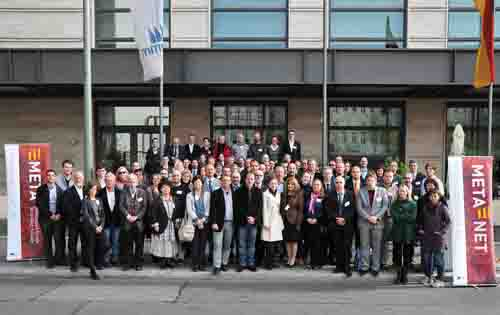
\includegraphics[width=\textwidth]{../_media/meta-net_team.jpg}
  \caption{Prop de 100 experts en tecnologies del llenguatge -- representants dels països i idiomes representats a META-NET --  van discutir i concloure els resultats clau i missatges de la sèrie de llibres blancs a la reunió de META-NET a Berlin, Alemanya el 21/22 d'octubre de 2011. ---
 \textcolor{grey1}{About 100 language technology experts -- representatives of the countries and languages represented in META-NET -- discussed and finalised the key results and messages of the White Paper Series at a META-NET meeting in Berlin, Germany, on October 21/22, 2011.}}
  \medskip
  \colorrule{grey3}{\textwidth}{1.5pt}
\end{figure*}

\cleardoublepage

\bsection[La sèrie de llibres blancs de META-NET -- The META-NET White Paper Series]{La sèrie de llibres blancs de META-NET --- The META-NET\ \ \ \ \ \ White Paper Series}
\label{whitepaperseries}

\vspace*{-5mm}
\centering
  \setlength{\tabcolsep}{2em}
  \begin{tabularx}{\textwidth}{lllll} \toprule\addlinespace
  %\begin{tabulary}{170mm}{LLL} \toprule
  Alemany & German & Deutsch\\
  Anglès & English & English\\
  Basc & Basque & euskara\\
  Búlgar & Bulgarian & български \\
  Català & Catalan & català\\
  Croat & Croatian & hrvatski\\
  Danès & Danish & dansk\\
  Eslovac & Slovak & slovenčina\\
  Eslovè & Slovene & slovenščina\\
  Espanyol & Spanish & español\\
  Estonià & Estonian & eesti\\
  Finès & Finnish & suomi\\
  Francès & French & français\\
  Gallec & Galician & galego\\
  Grec & Greek & ελληνικά\\
  Holandès & Dutch & Nederlands\\
  Hongarès & Hungarian & magyar\\ 
  Irlandès & Irish & Gaeilge\\
  Islandès & Icelandic & íslenska\\
  Italià & Italian & italiano\\
  Letó & Latvian & latviešu valoda\\
  Lituà & Lithuanian & lietuvių kalba\\
  Maltès & Maltese & Malti\\
  Noruec Bokmål & Norwegian Bokmål & bokmål\\
  Noruec Nynorsk & Norwegian Nynorsk & nynorsk\\
  Polonès & Polish & polski\\
  Portuguès & Portuguese & português\\
  Romanès & Romanian & română\\
  Serbi & Serbian & српски\\
  Suec & Swedish & svenska\\
  Txec & Czech & čeština\\  \addlinespace \bottomrule
\end{tabularx}
